% ============================================================================
% TCC — Big Five x Perfil de Investidor: simulação com agentes de IA
% Template oficial do DCC/UFRRJ (projetofinal-dcc.cls, Prof. Filipe Braida),
% adaptado do modelo original do DCC/UFRJ.
% Fonte do template: https://github.com/filipebraida/monografia-latex
%
% Compilação: pdflatex + bibtex + pdflatex x2, de dentro de monografia/
% ============================================================================
\documentclass{projetofinal-dcc}

% ---------------------------------------------------------------------------
% Pacotes
% ---------------------------------------------------------------------------
\usepackage{lmodern}
% inputenc/fontenc/graphicx/amsmath/hyperref/color/booktabs/xcolor/abntex2cite/
% microtype/csquotes/acronym/ccaption já são carregados por projetofinal-dcc.cls

% Quadros (ABNT: informação textual, diferente de Tabela, que é numérica).
% Numeração por capítulo, como figuras e tabelas, e lista própria.
\usepackage{newfloat}
\DeclareFloatingEnvironment[fileext=loq, listname={Lista de Quadros}, name=Quadro, within=chapter]{quadro}

% Caixa para prompts enviados ao modelo de linguagem: fonte monoespaçada
% dentro de um quadro com borda, padrão usual de apresentação de prompts.
\usepackage[most]{tcolorbox}
\newtcolorbox{promptbox}{
    enhanced, sharp corners,
    colback=gray!6, colframe=gray!55, boxrule=0.6pt,
    left=2.5mm, right=2.5mm, top=1.5mm, bottom=1.5mm,
    fontupper=\ttfamily\footnotesize,
    before upper={\setlength{\parindent}{0pt}\setlength{\parskip}{0.5em}\raggedright}
}
% Trecho variável dentro de um prompt (preenchido pelo código para cada agente)
\newcommand{\campo}[1]{\textit{\{#1\}}}

% Marcador visual de pendência (não deve aparecer na versão final)
\newcommand{\FIXME}[1]{\textbf{\textcolor{red}{[PENDENTE: #1]}}}

% ---------------------------------------------------------------------------
% Configurações de aparência do PDF
% ---------------------------------------------------------------------------
\hypersetup{
    pdftitle={Traços de Personalidade Big Five e Perfil de Investidor: uma Simulação com Agentes de Inteligência Artificial},
    pdfauthor={Mariana Ferreira Ferrarez Ribeiro},
    pdfkeywords={Big Five}{Personalidade}{Perfil de Investidor}{Inteligência Artificial}{LLM}{Finanças Comportamentais},
    colorlinks=true,
    linkcolor=black,
    citecolor=black,
    urlcolor=black,
    filecolor=black,
    bookmarksdepth=4
}

% Números da verificação do sorteio (\aleat...), gerados por analise_aleatorizacao.py
% Gerado por analise_aleatorizacao.py -- não editar à mão; rode o script de novo.
\newcommand{\aleatN}{300}
\newcommand{\aleatContagemMin}{92}
\newcommand{\aleatContagemMax}{112}
\newcommand{\aleatPFreqMin}{0,326}
\newcommand{\aleatRhoMax}{0,103}
\newcommand{\aleatPRhoMin}{0,075}
\newcommand{\aleatCramerMax}{0,104}
\newcommand{\aleatVIFMin}{1,000}
\newcommand{\aleatVIFMax}{1,014}
\newcommand{\aleatCombUnicas}{174}
\newcommand{\aleatCombEsperado}{172,4}
\newcommand{\aleatNSim}{10.000}
\newcommand{\aleatSomaMedia}{9,96}
\newcommand{\aleatSomaDP}{1,87}
\newcommand{\aleatPMetadesMin}{0,444}
\newcommand{\aleatPMetadesMax}{0,780}
\newcommand{\aleatAberturaCoefSimples}{+1,722}
\newcommand{\aleatAberturaCoefMulti}{+1,716}
\newcommand{\aleatQUmChi}{6,72}
\newcommand{\aleatQUmP}{0,081}
\newcommand{\aleatDominanteChi}{3,73}
\newcommand{\aleatDominanteP}{0,443}
\newcommand{\aleatNeuroBP}{0,026}


% ---------------------------------------------------------------------------
% Início do documento
% ---------------------------------------------------------------------------
\begin{document}

% título é obrigatório
\title{Traços de Personalidade Big Five e Perfil de Investidor: uma Simulação com Agentes de Inteligência Artificial}

% autor é obrigatório; agradecimentos entram como 2º argumento
\author{Mariana Ferreira Ferrarez Ribeiro}{% ----------------------------------------------------------
% AGRADECIMENTOS — obrigatório neste template (projetofinal-dcc.cls chama
% \makethankspage sem condicional); conteúdo puro, sem ambiente (é o 2º
% argumento de \author{}{} em main.tex).
% ----------------------------------------------------------
Agradeço, antes de tudo, a Deus, por me conceder a oportunidade de viver
esta conquista e por me sustentar ao longo de toda essa caminhada.

À minha família, a quem devo tudo o que sou e que sempre esteve ao meu
lado. Ao meu pai, Luciano, que me ensinou tudo o que sei; à minha mãe,
Luana, que me ensina diariamente o verdadeiro significado do amor; e ao
meu irmão, Davi, por todo o carinho, companheirismo e por ser alguém com
quem sei que sempre posso contar. Obrigada por serem meu alicerce, por
acreditarem em mim e por fazerem parte de cada passo dessa trajetória.
Aos meus avós, agradeço por todas as orações, pelo carinho e por sempre
torcerem por mim.

Ao meu orientador, Leandro Guimarães Marques Alvim, agradeço pela
orientação, disponibilidade, paciência e pelas contribuições ao longo do
desenvolvimento deste trabalho.

Aos Pupilos do Hélio, Hélio, Pedro Guedes, Rafael Vieira, Rafael
França (Mage), Pedro Albuquerque (Albergue), Davi e Helcio,
agradeço por terem tornado essa caminhada mais leve e especial.
}

% orientador é obrigatório
\advisor[Prof.]{Leandro Guimarães Marques Alvim,~D.Sc.}{DCC~-~UFRRJ}{}

% banca (máx. 3 membros; orientador já é adicionado automaticamente)
\banca[Prof.]{Filipe Braida do Carmo,~D.Sc.}{DCC~-~UFRRJ}
\banca[Prof.]{Ronaldo e Silva Vieira,~M.Sc.}{DCC~-~UFRRJ}

\dept{dcc}
\curso{cbcc}

\location{Nova Iguaçu}{RJ}{Brasil}

% mês e ano de defesa
\date{Dezembro}{2026}
\maketitle

\startdocument
%%%%%%%%%%%%%%%%%%%%%%%%%%%%%%%%%%%%%%%%%%%%%%%%%%%%%%%%%%%%
%A G R A D E C I M E N T O S
%%%%%%%%%%%%%%%%%%%%%%%%%%%%%%%%%%%%%%%%%%%%%%%%%%%%%%%%%%%%
\makethankspage

%%%%%%%%%%%%%%%%%%%%%%%%%%%%%%%%%%%%%%%%%%%%%%%%%%%%%%%%%%%%
%R E S U M O  /  A B S T R A C T
%%%%%%%%%%%%%%%%%%%%%%%%%%%%%%%%%%%%%%%%%%%%%%%%%%%%%%%%%%%%
\begin{abstract}{
      Este trabalho investiga se traços de personalidade do modelo Big Five,
    induzidos por instrução (\textit{prompt}) em agentes de inteligência
    artificial baseados em modelos de linguagem de grande escala (LLM),
    predizem o perfil de investidor desses agentes, medido pelo instrumento
    IPA (Índice de Perfil do Investidor). A pergunta é desdobrada em três
    questões: se os LLMs simulam consistentemente os traços solicitados,
    quais associações entre personalidade e perfil de investidor são
    robustas e em que medida elas dependem do modelo e dos parâmetros de
    geração. Na análise principal, foram gerados 300 agentes com o modelo
    \texttt{llama3.1:8b}, cada um com níveis (Baixo/Médio/Alto) sorteados
    para os cinco traços. Os agentes responderam ao BFI-44 (autorrelato de
    personalidade, usado como checagem de manipulação) e ao IPA. A análise
    foi repetida com outras temperaturas de geração, com um novo sorteio de
    perfis e com outros modelos de linguagem. A indução de personalidade foi
    fiel nos cinco traços ($\rho$ entre 0,813 e 0,929). Na análise
    principal, Abertura à Experiência, Extroversão, Consciência e
    Neuroticismo predisseram significativamente o escore do IPA (regressão
    OLS, $R^2=0{,}459$; $p<0{,}001$), mas apenas Abertura à Experiência e
    Extroversão se mantiveram significativas em todas as rodadas da análise
    de robustez (temperaturas, sorteio e modelos); os efeitos de Consciência e
    Neuroticismo mostraram-se instáveis, e Amabilidade não teve efeito
    consistente. O perfil de investidor absoluto atribuído a uma mesma
    personalidade variou fortemente entre modelos. O achado de Abertura à
    Experiência converge com De Bortoli et al. (2019), Jiang, Peng e Yan
    (2024) e estudos recentes com LLMs. Conclui-se que agentes de IA
    baseados em LLM, quando adequadamente induzidos e com a manipulação
    verificada, reproduzem a direção de parte das relações conhecidas entre
    personalidade e tolerância ao risco, mas que o nível de risco que
    declaram é, em grande parte, uma característica do modelo usado.

    \vspace{\baselineskip}

    \noindent
    \textbf{Palavras-chave}: Big Five. Perfil de investidor. Inteligência
    artificial. Modelos de linguagem. Finanças comportamentais.

}
\end{abstract}

\begin{englishabstract}{
      \begin{otherlanguage*}{english}
        This work investigates whether Big Five personality traits, induced
        through prompting in artificial intelligence agents based on large
        language models (LLMs), predict the investor profile of these
        agents, as measured by the IPA (Investor Profile Index) instrument.
        The question is broken down into three: whether LLMs consistently
        simulate the requested traits, which associations between
        personality and investor profile are robust, and how much they
        depend on the model and on generation parameters. In the main
        analysis, 300 agents were generated with the \texttt{llama3.1:8b}
        model, each with randomly assigned levels (Low/Medium/High) for the
        five traits, which answered the BFI-44 (personality self-report,
        used as a manipulation check) and the IPA. The analysis was
        repeated with other generation temperatures, with a new draw of
        personality profiles, and with other language models. Personality
        induction was faithful for all five traits ($\rho$ between 0.813
        and 0.929). In the main analysis, Openness to Experience,
        Extraversion, Conscientiousness, and Neuroticism significantly
        predicted the IPA score (OLS regression, R² = 0.459; p < 0.001),
        but only Openness to Experience and Extraversion remained
        significant across all temperatures, draws, and models tested; the
        Conscientiousness and Neuroticism effects proved unstable, and
        Agreeableness showed no consistent effect. The absolute investor
        profile assigned to the same personality varied strongly across
        models. The Openness to Experience finding converges with De
        Bortoli et al. (2019), Jiang, Peng and Yan (2024), and recent
        studies with LLMs. It is concluded that LLM-based AI agents, when
        properly induced and with verified manipulation, reproduce the
        direction of part of the known relationships between personality
        and risk tolerance, but that the level of risk they declare is
        largely a property of the model used.

        \vspace{\baselineskip}

        \noindent
        \textbf{Keywords}: Big Five. Investor profile. Artificial
        intelligence. Language models. Behavioral finance.
    \end{otherlanguage*}

}
\end{englishabstract}

%%%%%%%%%%%%%%%%%%%%%%%%%%%%%%%%%%%%%%%%%%%%%%%%%%%%%%%%%%%%
%L I S T A S
%%%%%%%%%%%%%%%%%%%%%%%%%%%%%%%%%%%%%%%%%%%%%%%%%%%%%%%%%%%%
\makefigurespage
\addcontentsline{toc}{chapter}{Lista de Quadros}
\listofquadros
\pagebreak
\maketablespage

% Abreviaturas e siglas (ordem alfabética)
% O pacote acronym é carregado com [printonlyused] pela classe
% (projetofinal-dcc.cls), que só lista uma sigla se \ac{} for usado no
% corpo do texto. A monografia escreve as siglas direto na prosa (ex.
% "IPA"), não via \ac{IPA}, então a lista sairia vazia por padrão.
% \acused{} NÃO resolve isso (testado e confirmado: só marca a sigla como
% "já introduzida" para fins de \ac{} subsequente, não ativa o \write no
% .aux que o printonlyused verifica -- ver acronym.sty, comandos
% \acused/\AC@logged). A forma robusta e independente de número de
% passadas é desligar \AC@printonlyused localmente só dentro deste bloco.
\makeatletter
\AC@printonlyusedfalse
\makeatother
\makeabrevpage{
  \begin{acronym}[ANBIMA]
    \acro{ABNT}{Associação Brasileira de Normas Técnicas}
    \acro{ANBIMA}{Associação Brasileira das Entidades dos Mercados Financeiro e de Capitais}
    \acro{BFI}{Big Five Inventory}
    \acro{CPU}{Central Processing Unit}
    \acro{CRT}{Cognitive Reflection Test}
    \acro{GPU}{Graphics Processing Unit}
    \acro{IA}{Inteligência Artificial}
    \acro{IPA}{Índice de Perfil do Investidor}
    \acro{LLM}{Large Language Model (Modelo de Linguagem de Grande Escala)}
    \acro{OLS}{Ordinary Least Squares (Mínimos Quadrados Ordinários)}
    \acro{RQ}{Research Question (Questão de Pesquisa)}
    \acro{TCC}{Trabalho de Conclusão de Curso}
    \acro{UFRRJ}{Universidade Federal Rural do Rio de Janeiro}
  \end{acronym}
}

% Símbolos (ordem alfabética; notação estatística usada no trabalho)
\makesymbolspage{
  \begin{acronym}[XXXX]
    \acro{F}{Estatística F do teste de significância global da regressão OLS}
    \acro{N}{Tamanho da amostra}
    \acro{p}{Valor-p (nível descritivo de significância estatística)}
    \acro{R2}[$R^2$]{Coeficiente de determinação da regressão OLS}
    \acro{rho}[$\rho$]{Coeficiente de correlação de Spearman}
  \end{acronym}
}
\makeatletter
\AC@printonlyusedtrue
\makeatother

\maketocpage

%%%%%%%%%%%%%%%%%%%%%%%%%%%%%%%%%%%%%%%%%%%%%%%%%%%%%%%%%%%%
%C O N T E Ú D O
%%%%%%%%%%%%%%%%%%%%%%%%%%%%%%%%%%%%%%%%%%%%%%%%%%%%%%%%%%%%
\startcontent
% Folga extra na quebra de linha para parágrafos com termos longos em
% \texttt (nomes de modelos), evitando linhas que ultrapassam a margem.
\setlength{\emergencystretch}{3em}
% ============================================================================
% CAPÍTULO 1 — INTRODUÇÃO
% ============================================================================
\chapter{Introdução}
\label{cap:introducao}

A teoria financeira tradicional parte do pressuposto de que investidores
tomam decisões de forma racional, buscando maximizar sua utilidade
esperada a partir das informações disponíveis. As finanças comportamentais
questionam esse pressuposto ao mostrar que fatores psicológicos, como
heurísticas, vieses cognitivos e diferenças individuais de personalidade,
influenciam sistematicamente as decisões financeiras, afastando-as do
ideal puramente racional \cite{jiangpengyan2024}. Dentro dessa perspectiva,
um instrumento amplamente utilizado pelo mercado financeiro para orientar
recomendações de investimento é o \textbf{perfil de investidor}: um
levantamento do quanto um indivíduo está disposto e é capaz de tolerar
risco, tipicamente classificado em categorias como conservador, moderado e
arrojado. No Brasil, a verificação desse perfil (\textit{suitability}) é
inclusive uma exigência regulatória para instituições que prestam serviços
de investimento \cite{cvm30_2021}.

Ainda que o perfil de investidor seja operacionalizado, em geral, por meio
de questionários padronizados sobre horizonte de tempo, patrimônio e
tolerância declarada ao risco, uma linha de pesquisa em finanças
comportamentais busca relacionar esse perfil a características de
personalidade mais estáveis do indivíduo, em particular ao modelo
\textbf{Big Five} de personalidade (Capítulo \ref{cap:referencial}).
Jiang, Peng e Yan \cite{jiangpengyan2024}, em uma pesquisa com 3.325
investidores reais, encontraram evidências de que traços de
personalidade, destacadamente Abertura à Experiência e Neuroticismo,
se relacionam com crenças sobre o mercado, aversão ao risco e alocação de
carteira, com poder explicativo comparável ao de variáveis demográficas
tradicionais. De Bortoli et al. \cite{debortoli2019}, em um estudo com
124 estudantes universitários, verificaram que, entre os cinco traços,
apenas Abertura à Experiência se associou ao perfil de risco observado em
uma simulação de investimento. Esses dois estudos servem de base teórica e metodológica
para o presente trabalho e são discutidos em detalhe no Capítulo
\ref{cap:referencial}.

Paralelamente, o avanço recente de modelos de linguagem de grande escala
(\textit{Large Language Models}, doravante LLMs) tem aberto uma nova possibilidade
metodológica para as ciências comportamentais: usar agentes de
inteligência artificial como respondentes simulados em pesquisas que, com
sujeitos humanos, demandariam tempo e recursos consideráveis. Um LLM pode
ser instruído, por meio de um \textit{prompt} de sistema, a responder como
se tivesse determinadas características, como um perfil de
personalidade específico, o que permite gerar, em escala e a baixo
custo, um número arbitrariamente grande de "agentes" com personalidade
controlada experimentalmente. Essa abordagem carrega limitações de
validade externa evidentes (um agente de IA não é um investidor real, e
seu comportamento reflete os dados e vieses do modelo que o gera), mas
oferece, em contrapartida, um ambiente de simulação totalmente controlado:
o nível de personalidade "verdadeiro" de cada agente é conhecido por
construção, sem o erro de medida inerente a autorrelatos humanos.

É nesse cruzamento entre a literatura de personalidade e perfil de
investidor, de um lado, e o uso de LLMs como sujeitos simulados, de outro,
que se insere este trabalho: agentes de IA recebem uma personalidade
Big Five induzida por instrução, respondem a um questionário de
autorrelato de personalidade (para verificar se a personalidade induzida
foi de fato "incorporada" pelo agente) e a um questionário de perfil de
investidor, e a relação entre o nível de personalidade induzido e o perfil
de investidor obtido é analisada estatisticamente, em busca de padrões
comparáveis aos encontrados por Jiang, Peng e Yan \cite{jiangpengyan2024} e
De Bortoli et al. \cite{debortoli2019}.

\section{Problema de pesquisa}

A pergunta de pesquisa que orienta este trabalho é: \textbf{níveis
induzidos de personalidade Big Five em agentes de inteligência artificial
predizem o escore do questionário de perfil de investidor?}

Essa pergunta geral é desdobrada em três questões de pesquisa (RQ, do
inglês \textit{research questions}), respondidas ao longo do trabalho e
retomadas de forma explícita no Capítulo \ref{cap:conclusao}:

\begin{description}
    \item[RQ1:] Os LLMs conseguem simular consistentemente os traços de
    personalidade solicitados?
    \item[RQ2:] Quais associações entre personalidade induzida e perfil de
    investidor são robustas?
    \item[RQ3:] Quanto essas associações e os perfis financeiros dependem
    do modelo e dos parâmetros de geração?
\end{description}

A RQ1 trata da validade da própria simulação: sem uma indução de
personalidade verificada, nenhuma associação com o perfil de investidor
pode ser interpretada. A RQ2 separa, entre as associações observadas na
análise principal, as que se repetem sob diferentes condições das que
dependem de uma condição específica. A RQ3 avalia em que medida os
resultados são uma propriedade do modelo de linguagem e da configuração
de geração usados, e não da relação entre personalidade e risco em si.

Investigar essas questões contribui, por um lado, para avaliar se relações
já documentadas entre personalidade e comportamento de risco financeiro em
seres humanos se reproduzem em um ambiente de simulação com agentes de IA,
o que teria implicações tanto para a validade desse tipo de simulação
em pesquisas comportamentais quanto para a compreensão de possíveis vieses
desses modelos ao lidar com temas financeiros. Por outro lado, o desenho
experimental adotado (indução controlada de personalidade, seguida de
checagem de manipulação) oferece um paralelo metodológico direto ao
desenho de De Bortoli et al. \cite{debortoli2019}, permitindo comparação
relativamente direta entre os achados deste trabalho e os da literatura de
referência.

\section{Justificativa}

Este trabalho se justifica em três frentes complementares. Em primeiro
lugar, do ponto de vista teórico, ele testa, em um ambiente controlado e de
baixo custo, se relações já estabelecidas na literatura de finanças
comportamentais entre personalidade e comportamento de investimento se
replicam em um contexto de simulação com agentes de IA: gerar 300
respondentes simulados como os deste trabalho seria inviável em tempo e
custo com sujeitos humanos reais.

Em segundo lugar, do ponto de vista metodológico, o trabalho contribui
para a discussão, ainda incipiente, sobre o uso de LLMs como sujeitos
simulados em pesquisa comportamental: ao comparar explicitamente diferentes
modelos de linguagem quanto à qualidade da indução de personalidade (seção
\ref{sec:selecao-modelo}), o trabalho evidencia que essa qualidade não é
uniforme entre modelos e que a checagem de manipulação (verificar se o
agente de fato incorporou a personalidade pedida antes de interpretar
qualquer efeito sobre a variável dependente) é uma etapa metodológica
necessária, não apenas desejável, nesse tipo de simulação.

Em terceiro lugar, do ponto de vista prático, entender melhor os
determinantes psicológicos do perfil de investidor é relevante para a
adequação de produtos financeiros ao perfil do cliente (\textit{suitability})
e para iniciativas de educação financeira, ainda que as conclusões deste
trabalho, por partirem de agentes simulados, devam ser interpretadas como
exploratórias em relação a esse uso prático (ver limitações, seção
\ref{sec:limitacoes-pipeline}).

\section{Objetivos}

\subsection{Objetivo geral}

Investigar se traços de personalidade do modelo Big Five, induzidos por
instrução em agentes de inteligência artificial baseados em modelos de
linguagem de grande escala, predizem o perfil de investidor desses
agentes, medido por um questionário de perfil de investidor (IPA).

\subsection{Objetivos específicos}

\begin{enumerate}
    \item Induzir, por meio de instrução de sistema (\textit{prompt}),
    níveis (Baixo/Médio/Alto) dos cinco traços do Big Five em agentes
    baseados em LLM, e verificar a fidelidade dessa indução por meio de um
    questionário de autorrelato de personalidade (checagem de
    manipulação);
    \item Aplicar um questionário de perfil de investidor (IPA) aos
    mesmos agentes e obter, para cada um, um escore contínuo e uma
    classificação categórica (conservador, moderado ou arrojado);
    \item Testar a associação estatística (correlação de Spearman e
    regressão OLS) entre o nível de personalidade induzido e o escore do
    IPA, para cada um dos cinco traços do Big Five;
    \item Comparar os achados obtidos com os resultados relatados por
    De Bortoli et al. \cite{debortoli2019} e por Jiang, Peng e Yan
    \cite{jiangpengyan2024}, identificando convergências e divergências;
    \item Comparar o comportamento de diferentes modelos de linguagem
    (\texttt{llama3.2:1b}, \texttt{llama3.2:3b}, \texttt{gemma3:4b} e
    \texttt{llama3.1:8b}) quanto à qualidade da indução de personalidade,
    de modo a identificar em que medida o tamanho/família do modelo afeta a
    validade da simulação;
    \item Testar se induzir os 5 traços do Big Five simultaneamente no
    mesmo agente, em comparação a induzir apenas 1 traço por vez, afeta a
    qualidade da indução de personalidade ou a força da associação com o
    escore do IPA;
    \item Avaliar a robustez e a generalização das associações encontradas,
    repetindo a análise principal com outras temperaturas de geração, com
    um novo sorteio de perfis de personalidade e com outros modelos de
    linguagem.
\end{enumerate}

\section{Etapas do trabalho: seleção de modelo, piloto e análise principal}
\label{sec:trabalho-realizado-intro}

Como etapa preliminar à análise apresentada neste trabalho, foram testados
quatro modelos de linguagem distintos (\texttt{llama3.2:1b},
\texttt{llama3.2:3b}, \texttt{gemma3:4b} e \texttt{llama3.1:8b}) quanto à
sua capacidade de incorporar de forma consistente a personalidade induzida
por instrução (seção \ref{sec:selecao-modelo}). Esse levantamento mostrou
que a qualidade da indução de personalidade varia substancialmente entre
modelos: o modelo mais leve testado (\texttt{llama3.2:1b}) não incorporou
nenhum dos cinco traços de forma estatisticamente detectável, ao passo que
o modelo finalmente adotado como base para a análise principal deste
trabalho (\texttt{llama3.1:8b}) apresentou manipulação forte e
significativa em todos os cinco traços. Esse resultado é, em si, um
achado metodológico relevante: ele indica que o tamanho e a família do
modelo de linguagem são pré-requisitos para a validade desse tipo de
simulação, e que a checagem de manipulação não pode ser tratada como uma
formalidade dispensável.

O dataset descrito acima, baseado no instrumento de autorrelato BFI-10,
constitui o \textbf{estudo piloto} deste trabalho (seção
\ref{sec:bfi10-piloto}). Foi esse piloto que motivou tanto a escolha do
\texttt{llama3.1:8b} quanto o primeiro indício do achado central deste
trabalho, a associação entre Abertura à Experiência e o escore do IPA.

A partir desse piloto, a \textbf{análise principal} deste trabalho migrou
para um instrumento de autorrelato mais granular, o BFI-44 (44 itens,
seção \ref{sec:exp-a-b}), com dois desenhos de indução testados: o
\textbf{Experimento A}, que repete o desenho do piloto (os 5 traços
induzidos simultaneamente em cada agente) e constitui os resultados
principais reportados neste trabalho (Capítulo \ref{cap:resultados}); e
o \textbf{Experimento B}, um teste de robustez metodológica em que cada
agente tem apenas 1 traço induzido por vez, motivado pela pergunta de se
a indução simultânea de personalidade dilui o sinal de cada traço
individual. Os resultados do Experimento A confirmam e fortalecem o
achado de Abertura à Experiência observado no piloto, e revelam efeitos
adicionais de Extroversão, Consciência e Neuroticismo.

Por fim, uma \textbf{análise de robustez e generalização} repete o
Experimento A variando, uma de cada vez, a temperatura de geração do
modelo, o sorteio dos perfis de personalidade e o próprio modelo de
linguagem (três modelos abertos adicionais com N=300 e dois modelos
maiores, acessados por API, em caráter exploratório). Essa análise
mostra que os efeitos de Abertura à Experiência e de Extroversão se
mantêm em todas as condições testadas, ao passo que os de Consciência e
Neuroticismo mudam de significância e até de sinal conforme a condição,
e por isso são tratados neste trabalho como \textbf{resultados
instáveis} (Capítulos \ref{cap:resultados} e \ref{cap:discussao}).

\section{Estrutura do trabalho}

Além desta introdução, este trabalho está organizado em mais cinco
capítulos. O Capítulo \ref{cap:referencial} apresenta o referencial
teórico, cobrindo o conceito de personalidade e o modelo Big Five, o
conceito de perfil de investidor em finanças comportamentais, uma
revisão detalhada dos dois artigos-base que fundamentam as hipóteses deste
trabalho e os estudos recentes sobre personalidade induzida e risco em
LLMs. O Capítulo \ref{cap:metodologia} descreve o desenho experimental,
os instrumentos utilizados, o pipeline de geração dos agentes, o processo
de seleção do modelo de linguagem e os métodos de análise estatística. O
Capítulo \ref{cap:resultados} apresenta os resultados obtidos: checagem
de manipulação, distribuição do perfil de investidor, associações entre
personalidade induzida e escore do IPA e a análise de robustez e
generalização. O Capítulo \ref{cap:discussao}
interpreta esses resultados à luz da literatura de referência e discute as
limitações do estudo. Por fim, o Capítulo \ref{cap:conclusao} responde às
três questões de pesquisa, retoma os objetivos específicos, sintetiza as contribuições
do trabalho e aponta direções para pesquisas futuras.

% ============================================================================
% CAPÍTULO 2 — REFERENCIAL TEÓRICO
% ============================================================================
\chapter{Referencial Teórico}
\label{cap:referencial}

\section{Personalidade e o modelo Big Five}

\subsection{O que é personalidade}

A personalidade tem sido conceituada a partir de diversas perspectivas
teóricas e em diferentes níveis de abstração, e um dos níveis mais
estudados é o dos traços de personalidade \cite{johnsrivastava1999}. A
abordagem de traços, adotada neste trabalho, parte do princípio de que as
diferenças individuais de personalidade podem ser descritas por um número
pequeno de dimensões amplas e relativamente estáveis ao longo do tempo e
das situações, chamadas \textit{traços de personalidade}. Um traço não é
uma categoria discreta (a pessoa ``é'' ou ``não é'' extrovertida), mas um
\textit{continuum}: cada indivíduo pode ser posicionado em algum ponto
entre dois polos de cada dimensão.

\subsection{O modelo Big Five}

O modelo Big Five (também chamado de modelo dos cinco grandes fatores, ou
\textit{Five-Factor Model}) é a taxonomia de traços de personalidade em
torno da qual a área tem se aproximado de um consenso
\cite{johnsrivastava1999}. Ele emergiu da convergência de duas tradições
de pesquisa independentes: a abordagem lexical, que parte da análise
fatorial de adjetivos de personalidade usados na linguagem natural
\cite{goldberg1990}, e a abordagem baseada em questionários
psicométricos, como o \textit{Revised NEO Personality Inventory}
(NEO-PI-R) \cite{costamccrae1992}. Ambas as tradições chegaram a uma
estrutura de cinco dimensões amplas e relativamente independentes entre
si \cite{johnsrivastava1999}:

\begin{itemize}
    \item \textbf{Extroversão}: tendência a ser sociável, assertivo,
    ativo e a buscar estimulação e a companhia de outras pessoas, em
    oposição a um estilo mais reservado e independente;
    \item \textbf{Amabilidade} (também chamada de Afabilidade): tendência
    a ser cooperativo, confiante e altruísta em relação aos outros, em
    oposição a um estilo mais cético, competitivo ou antagônico;
    \item \textbf{Consciência}: tendência a ser organizado,
    disciplinado, orientado a objetivos e cumpridor de obrigações, em
    oposição a um estilo mais despreocupado ou impulsivo;
    \item \textbf{Neuroticismo}: tendência a experimentar emoções
    negativas (ansiedade, insegurança, instabilidade emocional) com maior
    frequência e intensidade, em oposição à estabilidade emocional;
    \item \textbf{Abertura à Experiência}: tendência à curiosidade
    intelectual, à imaginação e à apreciação por ideias, experiências
    estéticas e situações não convencionais, em oposição a um estilo mais
    convencional e pragmático.
\end{itemize}

Diversos instrumentos psicométricos foram desenvolvidos para medir esses
cinco traços, com diferentes números de itens e propósitos. O estudo
piloto deste trabalho utilizou o \textbf{BFI-10} \cite{rammstedtjohn2007},
uma versão reduzida de 10 itens (2 por traço) do \textit{Big Five
Inventory}, na tradução para o português utilizada por
\citeonline{debortoli2019} (detalhes no Capítulo \ref{cap:metodologia}). A
análise principal deste trabalho utiliza o \textbf{BFI-44}
\cite{johndonahuekentle1991}, versão completa de 44 itens, em uma versão em
português que segue a ordem e o conteúdo dos itens do instrumento
original; a validação psicométrica do BFI-44 para o Brasil foi feita por
\citeonline{andrade2008} (detalhes na seção \ref{sec:bfi44}). Na
literatura revisada neste capítulo aparece ainda o SAPA-20, a forma de 20
itens do \textit{SAPA Personality Inventory} \cite{condonrevelle2015},
utilizada por \citeonline{jiangpengyan2024}.

\section{Finanças comportamentais e perfil de investidor}

O \textbf{perfil de investidor} é o resultado de um processo de avaliação,
em geral um questionário estruturado, que busca estimar o quanto um
indivíduo está disposto a assumir risco em suas decisões de investimento
(tolerância) e é capaz de fazê-lo (capacidade financeira), classificando-o
tipicamente em categorias como conservador, moderado e arrojado. No
mercado financeiro brasileiro, essa avaliação, conhecida como
\textit{suitability}, é uma exigência regulatória: instituições que
distribuem produtos de investimento devem verificar a adequação desses
produtos ao perfil do cliente antes de recomendá-los
\cite{cvm30_2021}. O instrumento utilizado neste trabalho, o IPA (Índice
de Perfil do Investidor), segue esse modelo: é uma adaptação do
questionário de análise de perfil do investidor do Banco do Brasil,
alinhado às diretrizes da Associação Brasileira das Entidades dos
Mercados Financeiro e de Capitais (ANBIMA) e da \textit{International
Organization of Securities Commissions} (IOSCO), com oito perguntas
objetivas sobre horizonte de investimento, patrimônio, experiência prévia
e reação a cenários de perda (detalhes no Capítulo \ref{cap:metodologia}).

Uma linha de crítica relevante a esses instrumentos, levantada por
\citeonline{debortoli2019}, é que questionários de perfil de investidor
como o IPA, baseados em autorrelato sobre preferências e comportamentos
financeiros declarados, podem não capturar integralmente o comportamento
de risco \textit{real} de um indivíduo, medido, por exemplo, por meio de
simulações de investimento com dados reais de rentabilidade. No estudo
dos autores, o IPA teve relação coerente com o comportamento observado em
uma simulação de investimento, mas não foi suficiente, isoladamente, para
explicar todo esse comportamento, resultado que os autores interpretam
como evidência de que fatores adicionais, entre eles traços de
personalidade, contribuem para explicar o comportamento de risco além do
que o questionário de perfil de investidor capta sozinho. É essa lacuna,
a relação entre personalidade e perfil de investidor, que motiva a linha
de pesquisa revisada na seção seguinte.

\section{Personalidade e decisões de investimento: evidências empíricas}

\subsection{Jiang, Peng e Yan (2024)}
\label{sec:jiang}

\citeonline{jiangpengyan2024} investigaram a relação entre os cinco
traços do Big Five e o comportamento de investimento em uma amostra de
3.325 investidores americanos, associados da \textit{American Association
of Individual Investors} (AAII). Os traços de personalidade foram medidos
pelo SAPA-20 \cite{condonrevelle2015}, um instrumento de 20 itens (4 por
traço, escala de 1 a 6), e relacionados, por meio de regressões OLS com
os cinco traços como regressores simultâneos e controle por variáveis
demográficas, a quatro grupos de variáveis: crenças sobre o mercado
(retorno esperado, probabilidade de \textit{crash}, crescimento do
produto interno bruto, PIB, e inflação esperada), aversão ao risco,
comportamento de manada (\textit{herding}) e alocação de carteira
(percentual do patrimônio aplicado em ações).

Os principais achados dos autores são os seguintes. Primeiro,
\textbf{Neuroticismo} e \textbf{Abertura à Experiência} são os dois traços
que os próprios autores destacam como de maior poder explicativo sobre as
decisões de investimento; isso não significa que os outros três traços
tenham todos papel secundário ou nulo (ver o terceiro achado). Segundo,
os autores associam a cada um desses dois traços um canal distinto sobre
a alocação de carteira. No caso do Neuroticismo, o canal provável é o das
crenças: quem pontua mais alto nesse traço tende a avaliar o mercado de
forma mais pessimista, atribuindo maior probabilidade a um \textit{crash},
esperando menor crescimento do PIB e inflação mais alta, e aloca uma
proporção menor do patrimônio em ações. No caso da Abertura à
Experiência, o canal principal é a preferência por risco: Abertura mais
baixa está associada a maior aversão ao risco e a uma alocação menor em
ações, sem relação com o retorno médio esperado do mercado. Os autores
ressalvam, porém, que os dois traços continuam significativos mesmo
controlando a aversão ao risco e as expectativas de retorno, o que indica
a presença também de outros canais. Terceiro, Consciência tem
um padrão próprio, menos enfatizado pelos autores no resumo do artigo:
associa-se a expectativas \textit{mais otimistas} sobre o retorno
esperado do mercado e, ao mesmo tempo, a um investimento menor
em ações, efeito significativo na amostra americana e na alemã (nesta,
medido pela participação no mercado de ações), mas não na australiana,
em que só atinge significância ao nível de 10\% em uma das duas
especificações. Ou seja, Consciência tem efeito sobre a alocação de
carteira em duas das três amostras, na direção oposta à sugerida pelas
expectativas mais otimistas associadas a esse traço. Já Extroversão
associa-se a expectativas mais otimistas sobre o mercado (retorno
esperado e crescimento do PIB) e a menor aversão ao risco declarada, mas,
ao contrário de Consciência, sem efeito significativo sobre a
alocação de carteira nas amostras americana e australiana; apenas na
amostra alemã, em que a variável é a participação no mercado de ações,
Extroversão aparece associada negativamente a essa participação. Quanto
à Amabilidade, o traço está associado a maior aversão ao risco declarada
nas perguntas hipotéticas da pesquisa, mas sem reflexo na alocação real
de carteira; os autores não encontram evidência de que ele tenha papel
direto nas decisões financeiras. Por último, os autores
relatam que Neuroticismo e Extroversão também se associam a maior
comportamento de manada, e que o poder explicativo conjunto dos cinco
traços sobre as crenças do investidor é comparável ao de todas as
variáveis demográficas combinadas (gênero, idade, renda, riqueza,
educação e localização), resultado que os autores replicaram em uma
amostra de investidores chineses. Já as associações de Neuroticismo e
Abertura à Experiência com o investimento em ações foram replicadas em
amostras representativas da Austrália e da Alemanha.

\subsection{De Bortoli, da Costa Jr., Goulart e Campara (2019)}

\citeonline{debortoli2019} compararam quatro paradigmas teóricos
distintos, a saber: a Teoria da Perspectiva, o questionário de perfil de
investidor IPA (Banco do Brasil/ANBIMA), o BFI-10 (Big Five) e o
\textit{Cognitive Reflection Test} (CRT), um teste de reflexão
cognitiva, quanto à sua capacidade de explicar o perfil de risco
\textit{real} de 124 estudantes de graduação da Universidade Federal de
Santa Catarina (UFSC). Esse perfil de risco real foi medido por meio de
uma simulação computacional de investimento (\textit{ExpEcon}, 18
períodos), com ativos oferecidos pelo Banco do Brasil e dados históricos
reais de rentabilidade, e não apenas por autorrelato. A participação foi
voluntária e sem nenhum tipo de incentivo material aos participantes.

Para o Big Five, os autores utilizaram o BFI-10 e categorizaram o escore
de cada traço em três níveis (Baixo, Moderado e Alto), em vez de
tratá-lo como uma variável contínua. Essa categorização é a base direta
do desenho experimental adotado neste trabalho, que usa três níveis
equivalentes (Baixo, Médio e Alto), com a diferença de que aqui os
níveis são induzidos, e não medidos (Capítulo \ref{cap:metodologia}).
Usando regressão logística ordenada (variável dependente: o perfil de
risco obtido no simulador, em três categorias), os autores encontraram
que, de todos os cinco traços do Big Five, apenas Abertura à Experiência
foi estatisticamente significativa: maior
Abertura esteve associada a maior chance de o participante apresentar um
perfil ``arrojado'' no simulador. Os outros quatro traços não
apresentaram relação significativa com o perfil de risco real.

Os autores relatam ainda dois achados adicionais relevantes para este
trabalho. Primeiro, como já mencionado na seção anterior, o IPA não
explicou isoladamente o comportamento de risco real dos participantes.
Segundo, no questionário de Teoria da Perspectiva aplicado antes da
simulação, 92\% dos participantes responderam predominantemente de forma
incompatível com a Teoria da Utilidade Esperada, um resultado consistente
com a Teoria da Perspectiva e que reforça, de forma mais ampla, a relevância de fatores
psicológicos, e não apenas racionais e econômicos, na explicação do
comportamento de investimento.

\subsection{Síntese e hipóteses de referência}
\label{sec:hipoteses-referencia}

Os dois estudos revisados nesta seção convergem parcialmente, mas não
totalmente, quanto a quais traços do Big Five são relevantes para o
comportamento de investimento, o que já é, em si, um indício de que essa
relação pode depender do contexto, da amostra e de como o comportamento de
risco é medido: por autorrelato de alocação de carteira, em
\citeonline{jiangpengyan2024}, e por simulação de investimento com dados
históricos reais, em \citeonline{debortoli2019}. Ainda assim,
quatro pontos de comparação emergem como \textbf{hipóteses de
referência} para os resultados deste trabalho (Capítulo
\ref{cap:discussao}):

\begin{itemize}
    \item \textbf{Abertura à Experiência} é o traço mais consistentemente
    associado à tolerância ao risco de investimento nos dois estudos:
    significativo tanto em \citeonline{debortoli2019} (o único traço
    significativo do estudo) quanto em \citeonline{jiangpengyan2024} (um
    dos dois traços com maior poder explicativo);
    \item \textbf{Neuroticismo} tem papel relevante em
    \citeonline{jiangpengyan2024} (via crenças pessimistas sobre o
    mercado), mas não foi significativo em \citeonline{debortoli2019}, uma
    divergência que pode refletir diferenças de amostra (investidores
    reais vs. estudantes) ou de variável dependente (crenças e alocação
    declarada vs. comportamento em simulação);
    \item \textbf{Consciência} segue o mesmo padrão de divergência que o
    Neuroticismo: tem efeito negativo sobre a alocação de carteira em
    \citeonline{jiangpengyan2024} (em duas das três amostras do artigo),
    mas não foi significativa em \citeonline{debortoli2019};
    \item \textbf{Amabilidade} não teve relação significativa em
    \citeonline{debortoli2019} e, em \citeonline{jiangpengyan2024},
    associou-se a maior aversão ao risco declarada, sem efeito sobre a
    alocação de carteira.
\end{itemize}

A categorização dos níveis de personalidade em Baixo/Moderado/Alto
adotada por \citeonline{debortoli2019} e a regressão OLS com os cinco
traços como regressores simultâneos empregada por
\citeonline{jiangpengyan2024} formam, em conjunto, a base metodológica do
desenho experimental adotado neste trabalho, detalhado no Capítulo
\ref{cap:metodologia}.

\section{Agentes de IA e modelos de linguagem como sujeitos simulados}

A pesquisa revisada na seção anterior foi conduzida com sujeitos humanos,
e nenhum dos dois artigos-base trata do uso de modelos de linguagem como
respondentes. Justificar a checagem de manipulação como etapa
metodológica necessária neste trabalho (seção \ref{sec:bfi44}) exige
recorrer a uma linha de pesquisa
distinta, ainda recente, sobre o uso de LLMs como sujeitos simulados em
ciências comportamentais.

\subsection{LLMs como sujeitos simulados}

\citeonline{argyle2023} cunharam o termo \textit{silicon sampling} para
descrever essa abordagem: ao condicionar um LLM (GPT-3) com descrições
sociodemográficas de participantes reais, principalmente do
\textit{American National Election Studies}, os autores obtiveram
distribuições de resposta fortemente correlacionadas com as das amostras
humanas originais. Esse resultado inaugural sustentou a expectativa de
que modelos de linguagem, adequadamente instruídos, poderiam funcionar
como substitutos de baixo custo para respondentes humanos em pesquisas de
opinião e comportamento. \citeonline{ong2024} situa esse uso dentro de
uma tipologia mais ampla, que divide a pesquisa com LLMs em três
paradigmas: \textit{GPT-ology}, LLMs como modelos computacionais e
\textit{silicon sampling} (LLMs simulando humanos). O autor destaca que
um mesmo experimento pode levar a inferências diferentes conforme a
pergunta de pesquisa e que, no caso do \textit{silicon sampling}, a
suposição de que as respostas do modelo reproduzem as respostas humanas
precisa ser testada, e não assumida.

Estudos subsequentes qualificam esse otimismo inicial. \citeonline{park2024}
reproduziram 14 estudos do projeto de replicação \textit{Many Labs 2}
usando GPT-3.5 e, entre os oito estudos que puderam ser analisados,
replicaram apenas 37,5\% dos resultados originais; mais relevante para
este trabalho, os autores documentaram que o modelo respondia a perguntas
sobre orientação política, preferências econômicas, julgamento e
filosofia moral com variação nula ou quase nula entre execuções,
convergindo para uma mesma resposta supostamente ``correta'', padrão que
chamam de efeito da ``resposta correta'' (\textit{correct answer
effect}) e que motiva a preocupação, expressa no título do artigo, com
uma diversidade de pensamento diminuída. \citeonline{petrov2024},
especificamente sobre instrumentos de personalidade, testaram GPT-3.5 e
GPT-4 respondendo a questionários padronizados de traços, incluindo o
Big Five, sob diferentes personas: no GPT-4, mas não no GPT-3.5,
descrições genéricas de pessoa produziram respostas com propriedades
psicométricas promissoras, ainda que imperfeitas, próximas de normas
humanas; já perfis demográficos específicos produziram propriedades
psicométricas ruins nos dois modelos. Os autores concluem que,
atualmente, quando um LLM é instruído a simular personas definidas por
perfis demográficos, suas respostas são sinais pobres dos traços latentes
que supostamente representariam.

Os achados de \citeonline{park2024} e \citeonline{petrov2024}, tomados em
conjunto, sustentam diretamente a necessidade da checagem de manipulação
adotada neste trabalho: se a capacidade de um LLM de incorporar uma
personalidade induzida não pode ser assumida \textit{a priori}, tampouco
pode ser assumida a validade de qualquer relação estatística observada
entre essa personalidade e uma variável dependente, sem antes confirmar
que a indução de fato ocorreu. A checagem de manipulação é, portanto,
uma condição para que os resultados do Capítulo \ref{cap:resultados}
sejam interpretáveis. Os três estudos empíricos citados acima
\cite{argyle2023,park2024,petrov2024} testam modelos da família GPT
(OpenAI), e não os modelos abertos usados neste trabalho (seções
\ref{sec:selecao-modelo} e \ref{sec:metodo-robustez}); os achados servem
como motivação e paralelo conceitual, não como previsão direta do
comportamento dos modelos efetivamente usados aqui. O próprio
\textit{pipeline} deste trabalho também documentou vieses de resposta
dos modelos (viés de centralidade e maior dificuldade com itens de
pontuação reversa em modelos menores), discutidos nas seções
\ref{sec:limitacoes-pipeline} e \ref{sec:vieses}.

\subsection{Personalidade induzida e risco em LLMs}
\label{sec:ref-llm-risco}

Dois estudos recentes aproximam essa linha de pesquisa do tema deste
trabalho, ao investigar especificamente a relação entre personalidade
induzida em LLMs e comportamento de risco financeiro.

\citeonline{borman2024} construíram personas de LLM a partir do modelo
Big Five, atribuindo a cada um dos cinco traços um nível Baixo, Médio ou
Alto e gerando as 243 combinações possíveis desses níveis. As personas
foram testadas com ChatGPT 3.5 e ChatGPT 4.0 (os autores reportam os
resultados do segundo), e a personalidade induzida foi validada por meio
de um teste de personalidade do modelo dos cinco fatores, uma checagem
de manipulação análoga à deste trabalho. As personas responderam a dois
instrumentos: um questionário comportamental curto, de nove perguntas
elaboradas principalmente a partir de estudos anteriores com humanos, e
uma tarefa simulada de investimento, criada pelos autores, em que cada
persona escolhia uma entre cinco empresas com retorno e fator de risco
informados, podendo optar por pesquisar sobre elas antes de decidir. A
relação entre traços e comportamentos foi estimada por regressão OLS nos
dois casos. No apetite ao risco, o questionário reproduziu a direção
esperada pela literatura humana em três traços (Abertura à Experiência,
Extroversão e Neuroticismo), mas não em Consciência e Amabilidade; já a
tarefa simulada reproduziu a direção esperada nos cinco traços. De forma
mais geral, os autores concluem que as personas representaram o
comportamento humano melhor na tarefa simulada do que no questionário.

\citeonline{hartley2025} estudaram a relação entre personalidade e
propensão ao risco em diversos LLMs comerciais (entre eles GPT-4o,
GPT-4o mini, GPT-4 Turbo, Claude 3 Sonnet, Claude 3 Haiku, Gemini 1.5 Pro
e Gemini 1.5 Flash), usando a Teoria da Perspectiva Cumulativa: o risco
é medido pelos parâmetros que melhor explicam o equivalente certo
informado pelo modelo para cada loteria, isto é, o valor garantido que
ele aceitaria no lugar de apostar. Diferentemente de
\citeonline{borman2024} e do Experimento A deste trabalho, a indução é
feita um traço por vez, com os demais mantidos constantes, por meio de
adjetivos bipolares em uma escala de intensidade de 1 a 9. Os autores
relatam três resultados relevantes para este trabalho. Primeiro, no
GPT-4o, Abertura à Experiência foi o único traço significativamente
correlacionado com os parâmetros de sensibilidade ao risco, em linha com
a literatura humana citada por eles; a comparação entre os cinco traços
é relatada pelos autores apenas para o GPT-4o, e nos demais modelos a
análise relatada concentra-se em Abertura à Experiência. Segundo, a
relação entre
personalidade e risco não foi uniforme entre modelos: as variantes
menores (GPT-4o mini e Claude 3 Haiku) não reproduziram o padrão das
variantes maiores, e alguns modelos apresentaram relações na direção
oposta à humana. Terceiro, sem intervenção de personalidade, a maioria
dos modelos se comportou de forma aproximadamente neutra ao risco.

Os dois estudos se diferenciam deste trabalho em pontos centrais. Usam
modelos proprietários comerciais, e não modelos de pesos abertos, como os
usados neste trabalho. Além disso, medem o risco por uma tarefa de escolha
entre empresas, em \citeonline{borman2024}, ou pelos equivalentes certos
de loterias informados pelo modelo, em \citeonline{hartley2025} e, no primeiro caso, também por um
questionário comportamental; nenhum deles usa um questionário de
\textit{suitability} como o IPA. Ainda assim, oferecem dois paralelos
diretos que são retomados no Capítulo \ref{cap:discussao}: o desenho de
indução de \citeonline{borman2024} (os cinco traços simultâneos em três
níveis) é essencialmente o mesmo do Experimento A (Capítulo
\ref{cap:metodologia}), e o papel de Abertura à Experiência como traço
mais associado ao risco aparece também em \citeonline{hartley2025}, no
GPT-4o.

% ============================================================================
% CAPÍTULO 3 — METODOLOGIA
% ============================================================================
\chapter{Metodologia}
\label{cap:metodologia}

\section{Delineamento geral}

Este trabalho utiliza uma abordagem de simulação: agentes de inteligência
artificial baseados em modelos de linguagem de grande escala (LLM) recebem,
via instrução de sistema (\textit{system prompt}), uma personalidade
induzida segundo o modelo Big Five, e em seguida respondem a dois
instrumentos: um de autorrelato de personalidade (checagem de manipulação)
e o Índice de Perfil do Investidor (IPA, variável dependente).

Trata-se de uma pesquisa \textbf{quantitativa}, pois a relação entre
personalidade induzida e escore do IPA é testada por meios estatísticos
(correlação de Spearman e regressão OLS, seção \ref{sec:analise-estatistica}),
não por análise qualitativa das respostas dos agentes. É também
\textbf{exploratória}, pois não foi encontrado um estudo anterior que
relacione personalidade induzida em agentes de IA a um questionário de
perfil de investidor (\textit{suitability}): os estudos mais próximos com
LLMs \cite{borman2024,hartley2025} medem o risco por tarefas de escolha,
pela avaliação de loterias e por questionários comportamentais, não por um questionário de
\textit{suitability}, e as hipóteses de referência deste trabalho
(Capítulo \ref{cap:referencial}) vêm de estudos com sujeitos humanos,
adaptadas por analogia.

O método é o de \textbf{simulação computacional controlada}:
diferentemente de um levantamento ou experimento com sujeitos humanos, o
nível de personalidade solicitado a cada agente é conhecido por construção
(definido pelo sorteio que gera o \textit{prompt}), o que elimina o erro
de medida da variável independente presente em estudos com autorrelato
humano. Em contrapartida, a validade das conclusões depende de o LLM realmente
incorporar, em sua geração de texto, a personalidade descrita no
\textit{prompt}; daí a necessidade da checagem de manipulação (seção
\ref{sec:bfi44}) e da verificação do desenho de indução do Experimento B (seção
\ref{sec:exp-a-b}).

\section{Instrumentos}

\subsection{Indução de personalidade (Baixo/Médio/Alto)}

Para cada um dos cinco traços do Big Five foram escritas três descrições
curtas (Baixo, Médio, Alto), baseadas no conteúdo dos itens do BFI-10
(seção \ref{sec:bfi10-piloto}). Essas
descrições são inseridas no \textit{system prompt} de cada agente para
induzir a personalidade (seção \ref{sec:prompts}). O Quadro
\ref{quadro:perfis-nivel} reproduz as 15 descrições.

\begin{quadro}[htbp]
    \caption{Descrições usadas para induzir cada nível de cada traço}
    \label{quadro:perfis-nivel}
    \centering
    \small
    \begin{tabular}{lp{12cm}}
        \toprule
        Nível & Descrição inserida no \textit{prompt} \\
        \midrule
        \multicolumn{2}{l}{\textbf{Extroversão}} \\
        Baixo & É uma pessoa reservada, prefere ambientes tranquilos e evita ser o centro das atenções. \\
        Médio & É uma pessoa equilibrada entre momentos sociais e momentos sozinha, nem muito reservada nem muito extrovertida. \\
        Alto & É uma pessoa sociável e extrovertida, gosta de estar com outras pessoas e de ambientes movimentados. \\
        \addlinespace
        \multicolumn{2}{l}{\textbf{Amabilidade}} \\
        Baixo & Tende a ser crítica com os outros, aponta defeitos com facilidade e confia pouco nas pessoas. \\
        Médio & Confia nas pessoas moderadamente: às vezes é crítica, às vezes é tolerante. \\
        Alto & Geralmente confia nas pessoas, é gentil e raramente é crítica ou aponta defeitos nos outros. \\
        \addlinespace
        \multicolumn{2}{l}{\textbf{Consciência}} \\
        Baixo & Tende a ser preguiçosa, desorganizada e costuma deixar tarefas inacabadas. \\
        Médio & É razoavelmente organizada, mas às vezes deixa tarefas para depois. \\
        Alto & É organizada e disciplinada, insiste até concluir qualquer tarefa ou trabalho. \\
        \addlinespace
        \multicolumn{2}{l}{\textbf{Neuroticismo}} \\
        Baixo & É uma pessoa relaxada, que controla bem o estresse e raramente fica nervosa. \\
        Médio & Mantém o equilíbrio emocional na maior parte do tempo, mas ocasionalmente fica ansiosa diante de problemas. \\
        Alto & Fica nervosa com facilidade e tem dificuldade para controlar o estresse e a ansiedade. \\
        \addlinespace
        \multicolumn{2}{l}{\textbf{Abertura à Experiência}} \\
        Baixo & Tem poucos interesses artísticos e pouca imaginação, prefere o familiar e o convencional. \\
        Médio & Tem alguns interesses artísticos e está moderadamente aberta a novas ideias e experiências. \\
        Alto & Tem uma imaginação fértil, muitos interesses artísticos e intelectuais, e gosta de experimentar coisas novas. \\
        \bottomrule
    \end{tabular}
    \legend{Fonte: elaborado pela autora.}
\end{quadro}

\subsection{Questionário de autorrelato: checagem de manipulação}
\label{sec:bfi44}

O instrumento utilizado como checagem de manipulação na análise principal
deste trabalho é o \textbf{BFI-44} \cite{johndonahuekentle1991}, versão
completa de 44 itens do \textit{Big Five Inventory}, em uma versão em
português que segue a ordem e o conteúdo dos 44 itens do instrumento
original, com a mesma escala de concordância de 1
(discordo totalmente) a 5 (concordo totalmente) usada no BFI-10 (seção
\ref{sec:bfi10-piloto}). A validação psicométrica do BFI-44 para o
Brasil foi conduzida por \citeonline{andrade2008}, com uma adaptação cuja
ordem e redação dos itens diferem em parte das usadas aqui; por isso, as
propriedades psicométricas relatadas por esse autor servem como
referência geral para o instrumento, e não como validação da versão
exata aplicada aos agentes. Cada um dos cinco traços é medido por um número
diferente de itens: Extroversão e Neuroticismo com 8 cada, Abertura à
Experiência com 10, e Amabilidade e Consciência com 9 cada, com itens
diretos e reversos em proporção variável por traço; a pontuação de cada traço é a média
dos seus itens, já com a reversão aplicada quando necessário (itens
reversos: escore final = 6 menos a resposta, mesma regra do BFI-10).

A Tabela \ref{tab:bfi44-resumo} resume o número de itens por traço, e o
Quadro \ref{quadro:bfi44-itens} reproduz as 44 afirmações, na forma em
que foram apresentadas aos agentes. As instruções e a escala de resposta
foram:

\begin{itemize}
    \item \textbf{Instruções}: ``As declarações a seguir dizem respeito à
    sua percepção sobre si mesmo em uma variedade de situações. Indique o
    número que melhor expressa sua opinião sobre você mesmo em cada
    afirmação.'' Frase-base: ``Eu me vejo como alguém que...'';
    \item \textbf{Escala de resposta}: 1 = Discordo totalmente; 2 =
    Discordo em parte; 3 = Nem concordo nem discordo; 4 = Concordo em
    parte; 5 = Concordo totalmente.
\end{itemize}

\begin{quadro}[htbp]
    \caption{Itens do BFI-44}
    \label{quadro:bfi44-itens}
    \centering
    \footnotesize
    \begin{tabular}{rp{7.6cm}lc}
        \toprule
        Item & Afirmação (``Eu me vejo como alguém que...'') & Traço & Escore \\
        \midrule
        1 & Gosta de conversar, é comunicativa. & Extroversão & D \\
        2 & Tende a criticar os outros. & Amabilidade & R \\
        3 & É minuciosa e detalhista no trabalho. & Consciência & D \\
        4 & Depressiva, triste. & Neuroticismo & D \\
        5 & É original, tem ideias novas. & Abertura à Experiência & D \\
        6 & É reservada. & Extroversão & R \\
        7 & É generosa e não é egoísta com outras pessoas. & Amabilidade & D \\
        8 & Pode ser desleixada para fazer as coisas. & Consciência & R \\
        9 & É tranquila, lida bem com estresse. & Neuroticismo & R \\
        10 & Se interessa por áreas diferentes do conhecimento. & Abertura à Experiência & D \\
        11 & É cheia de energia. & Extroversão & D \\
        12 & Inicia bate-boca com outros. & Amabilidade & R \\
        13 & É confiável no trabalho. & Consciência & D \\
        14 & Pode ser tensa. & Neuroticismo & D \\
        15 & É inovadora, pensa profundamente nas coisas. & Abertura à Experiência & D \\
        16 & Gera muito entusiasmo. & Extroversão & D \\
        17 & Desculpa, perdoa os outros. & Amabilidade & D \\
        18 & Tende a ser desorganizada. & Consciência & R \\
        19 & Se preocupa muito, em excesso. & Neuroticismo & D \\
        20 & Tem uma imaginação fértil. & Abertura à Experiência & D \\
        21 & Tende a ser quieta. & Extroversão & R \\
        22 & Geralmente confia, acredita nos outros. & Amabilidade & D \\
        23 & Tende a ser preguiçosa. & Consciência & R \\
        24 & É emocionalmente estável, não se perturba facilmente. & Neuroticismo & R \\
        25 & É inventiva. & Abertura à Experiência & D \\
        26 & É assertiva, não tem medo de expressar o que sente. & Extroversão & D \\
        27 & Às vezes é indiferente com os outros. & Amabilidade & R \\
        28 & Persevera até concluir as tarefas. & Consciência & D \\
        29 & É temperamental e instável emocionalmente. & Neuroticismo & D \\
        30 & Valoriza experiências artísticas e estéticas. & Abertura à Experiência & D \\
        31 & Às vezes é tímida, inibida. & Extroversão & R \\
        32 & É boa e atenciosa com quase todo mundo. & Amabilidade & D \\
        33 & Faz as coisas com eficiência. & Consciência & D \\
        34 & Se mantém calma em situações tensas. & Neuroticismo & R \\
        35 & Gosta de rotina. & Abertura à Experiência & R \\
        36 & É extrovertida e sociável. & Extroversão & D \\
        37 & Às vezes é grosseira com outras pessoas. & Amabilidade & R \\
        38 & Cumpre, finaliza os planos que faz. & Consciência & D \\
        39 & Fica nervosa facilmente. & Neuroticismo & D \\
        40 & Gosta de refletir, jogar com as ideias. & Abertura à Experiência & D \\
        41 & Tem poucos interesses artísticos. & Abertura à Experiência & R \\
        42 & Gosta de cooperar com outros. & Amabilidade & D \\
        43 & Se distrai facilmente. & Consciência & R \\
        44 & É sofisticada em arte, música ou literatura. & Abertura à Experiência & D \\
        \bottomrule
    \end{tabular}
    \legend{Fonte: itens conforme aplicados neste trabalho, versão em português do instrumento de \citeonline{johndonahuekentle1991}. D = escore direto; R = escore reverso.}
\end{quadro}

\begin{table}[htb]
    \caption{Número de itens do BFI-44, por traço}
    \label{tab:bfi44-resumo}
    \centering
    \begin{tabular}{lccc}
        \toprule
        Traço & Itens (total) & Diretos & Reversos \\
        \midrule
        Abertura à Experiência & 10 & 8 & 2 \\
        Amabilidade             & 9  & 5 & 4 \\
        Consciência             & 9  & 5 & 4 \\
        Extroversão             & 8  & 5 & 3 \\
        Neuroticismo            & 8  & 5 & 3 \\
        \bottomrule
    \end{tabular}
    \legend{Fonte: elaborado pela autora.}
\end{table}

Por ter mais itens por traço que o BFI-10 (2 por traço), o BFI-44 produz
uma média menos sensível ao ruído de um único item. Foi esse o principal
motivo para substituir o BFI-10, usado no estudo piloto, pelo BFI-44 na
análise principal: uma checagem de manipulação mais granular permite
distinguir com mais confiança entre ``o traço não foi incorporado pelo
agente'' e ``o traço foi incorporado, mas um ou dois itens específicos tiveram
resposta ruidosa'' (ver seção \ref{sec:limitacoes-pipeline} sobre o viés de
itens de pontuação reversa, que afeta mais um instrumento curto do que
um longo).

\subsection{Estudo piloto: BFI-10}
\label{sec:bfi10-piloto}

Antes da análise principal com o BFI-44 (seção \ref{sec:bfi44}), foi
conduzido um estudo piloto com o \textbf{BFI-10} \cite{rammstedtjohn2007},
versão reduzida de 10 itens do \textit{Big Five Inventory}, na tradução
em português reproduzida no Anexo 3 (material suplementar S2
Questionnaire) de \citeonline{debortoli2019}. Cada um dos cinco traços do Big Five
é medido por 2 itens, um com escore direto e outro com escore reverso, e
a pontuação da dimensão é a média dos seus 2 itens (mesma regra de
reversão do BFI-44).

O Quadro \ref{quadro:bfi10-itens} reproduz os 10 itens, com o traço
medido por cada um. As instruções e a escala de resposta são as mesmas
do BFI-44 (seção \ref{sec:bfi44}).

\begin{quadro}[htbp]
    \caption{Itens do BFI-10}
    \label{quadro:bfi10-itens}
    \centering
    \small
    \begin{tabular}{rp{7.2cm}lc}
        \toprule
        Item & Afirmação (``Eu me vejo como alguém que...'') & Traço & Escore \\
        \midrule
        1  & É reservado. & Extroversão & R \\
        2  & Geralmente confia nas pessoas. & Amabilidade & D \\
        3  & Tende a ser preguiçoso. & Consciência & R \\
        4  & É relaxado, controla bem o estresse. & Neuroticismo & R \\
        5  & Tem poucos interesses artísticos. & Abertura à Experiência & R \\
        6  & É sociável, extrovertido. & Extroversão & D \\
        7  & Tende a ser crítico com os outros (encontrar defeitos). & Amabilidade & R \\
        8  & Insiste até concluir a tarefa ou o trabalho. & Consciência & D \\
        9  & Fica nervoso facilmente. & Neuroticismo & D \\
        10 & Tem uma imaginação fértil. & Abertura à Experiência & D \\
        \bottomrule
    \end{tabular}
    \legend{Fonte: adaptado de \citeonline{debortoli2019}, Anexo 3, que traduz \citeonline{rammstedtjohn2007}. D = escore direto; R = escore reverso.}
\end{quadro}

O BFI-10 foi mantido deliberadamente como instrumento fixo em todos os
experimentos de comparação entre modelos de linguagem (seção
\ref{sec:selecao-modelo}): \texttt{llama3.2:1b}, \texttt{llama3.2:3b},
\texttt{gemma3:4b} e \texttt{llama3.1:8b}. Manter o mesmo instrumento de checagem
de manipulação em todos os modelos testados é o que torna válida a
comparação entre eles; usar instrumentos diferentes para modelos diferentes
confundiria efeito do modelo com efeito do instrumento. Os resultados do
estudo piloto (N=300) são
reportados na seção \ref{sec:resultados-piloto}, e permanecem relevantes
mesmo após a migração para o BFI-44: foram eles que motivaram a escolha do
\texttt{llama3.1:8b} como modelo principal (seção
\ref{sec:selecao-modelo}) e produziram o primeiro indício do achado
central deste trabalho (Abertura à Experiência), posteriormente
confirmado com o instrumento mais granular.

\subsection{Experimentos A e B: indução simultânea vs. isolada de traços}
\label{sec:exp-a-b}

Além da troca de instrumento (do BFI-10 para o BFI-44), dois desenhos de
indução foram testados com o BFI-44, mantendo o mesmo modelo
(\texttt{llama3.1:8b}) e N=300 em cada um:

\begin{itemize}
    \item \textbf{Experimento A (multi-traço)}: mesmo desenho do estudo
    piloto, em que os cinco traços variam Baixo/Médio/Alto de forma
    independente e simultânea em cada agente (seção
    \ref{sec:desenho-fatorial}). É o conjunto de dados da \textbf{análise
    principal} deste trabalho, reportado no Capítulo \ref{cap:resultados};
    \item \textbf{Experimento B (traço dominante)}: cada agente tem
    apenas um dos cinco traços sorteado para variar Baixo/Médio/Alto; os
    outros quatro permanecem fixos em ``Médio'' no \textit{system prompt}.
\end{itemize}

O Experimento B não substitui o A: é uma verificação do desenho de indução,
motivada pela possibilidade de que induzir os cinco traços
simultaneamente no mesmo \textit{prompt} dilua ou confunda o sinal de
cada traço individual, em comparação com a manipulação de apenas um traço
por vez. Se as correlações entre nível induzido e autorrelato (checagem
de manipulação) forem comparáveis nos dois desenhos, haverá evidência de
que a indução simultânea não compromete a qualidade da manipulação. A
indução simultânea é também o desenho mais próximo da personalidade
humana, na qual os cinco traços coexistem sempre em algum nível, e
corresponde à forma como os traços são medidos em
\citeonline{debortoli2019} e \citeonline{jiangpengyan2024}. Os resultados
dessa comparação estão na seção \ref{sec:resultados-exp-b} e são
interpretados no Capítulo \ref{cap:discussao}.

\subsection{IPA: perfil de investidor (variável dependente)}

O IPA é um instrumento de 8 perguntas objetivas (alternativas a--d),
adaptado do questionário de Análise de Perfil do Investidor do Banco do
Brasil, alinhado às diretrizes da ANBIMA e da IOSCO
(\textit{suitability}), conforme reproduzido no Anexo 5 de
\citeonline{debortoli2019}; o nome IPA (Índice de Perfil do Investidor)
é o adotado neste trabalho para esse instrumento. O Quadro
\ref{quadro:ipa-perguntas} reproduz as perguntas e as alternativas.

\begin{quadro}[htbp]
    \caption{Perguntas do IPA e alternativas}
    \label{quadro:ipa-perguntas}
    \centering
    \small
    \begin{tabular}{cp{13.4cm}}
        \toprule
        \multicolumn{2}{p{14.4cm}}{\textbf{1. Indique sua faixa etária.}} \\
        & a) Abaixo de 25 anos \quad b) De 25 a 40 anos \quad c) De 41 a 55 anos \quad d) Acima de 56 anos \\
        \addlinespace
        \multicolumn{2}{p{14.4cm}}{\textbf{2. Se você realizasse um investimento financeiro hoje (ex: fundos de investimento, poupança, CDI), qual o percentual do total de seu patrimônio que você aplicaria em investimentos?}} \\
        & a) Até 25\% \quad b) Entre 26\% e 50\% \quad c) Entre 51\% e 75\% \quad d) Mais de 75\% \\
        \addlinespace
        \multicolumn{2}{p{14.4cm}}{\textbf{3. Quando você realiza alguma aplicação (investimento financeiro), qual o prazo médio dos investimentos?}} \\
        & a) Indefinidamente, pois não tenho planos para utilização \quad b) No máximo 5 anos \quad c) No máximo 2 anos \quad d) No máximo 1 ano \\
        \addlinespace
        \multicolumn{2}{p{14.4cm}}{\textbf{4. Qual o principal objetivo de seus investimentos?}} \\
        & a) Obter rentabilidade superior à proporcionada por investimentos tradicionais de renda fixa, mesmo assumindo risco de possíveis perdas \quad b) Diversificar os investimentos \quad c) Formar uma reserva financeira para utilização futura \quad d) Preservar o patrimônio \\
        \addlinespace
        \multicolumn{2}{p{14.4cm}}{\textbf{5. Qual a sua melhor referência de rentabilidade?}} \\
        & a) Índices das Bolsas de Valores \quad b) Dólar \quad c) CDI \quad d) Poupança \\
        \addlinespace
        \multicolumn{2}{p{14.4cm}}{\textbf{6. Quais são as aplicações financeiras em que você tem maior conhecimento?}} \\
        & a) Fundo de Ações, Ações ou Derivativos \quad b) Fundos Multimercados, Cambiais, Dívida Externa ou Renda Fixa \quad c) CDB, Poupança ou Fundos Referenciados DI e Curto Prazo \quad d) Não tenho conhecimento \\
        \addlinespace
        \multicolumn{2}{p{14.4cm}}{\textbf{7. Você já investiu em ações ou Fundo de Ações?}} \\
        & a) Sim, pois a possibilidade de maiores rentabilidades me atraem muito \quad b) Sim, mas com receio \quad c) Não, mas poderia investir num momento oportuno \quad d) Não e não pretendo investir, pois não me agrada a ideia de estar sujeito a rentabilidade negativa \\
        \addlinespace
        \multicolumn{2}{p{14.4cm}}{\textbf{8. Caso a sua aplicação tivesse uma perda no curto prazo, qual seria o percentual aceitável?}} \\
        & a) Acima de 15\% \quad b) Até 15\% \quad c) Até 5\% \quad d) Não aceitaria perda \\
        \bottomrule
    \end{tabular}
    \legend{Fonte: adaptado de \citeonline{debortoli2019}, Anexo 5 (questionário de Análise de Perfil do Investidor do Banco do Brasil, alinhado à ANBIMA e à IOSCO).}
\end{quadro}

A pergunta 1 (faixa etária) foi atribuída aleatoriamente a cada agente, e
não respondida pelo modelo, por ser um dado demográfico inaplicável a
agentes de IA (ver seção \ref{sec:limitacoes-pipeline}).

\subsubsection{Regra de pontuação do IPA}
\label{sec:ipa-pontuacao}

O artigo de \citeonline{debortoli2019} não publica os pesos atribuídos a
cada alternativa nem os cortes de classificação de perfil
(conservador/moderado/arrojado) usados pelos autores. A regra de
pontuação descrita nesta seção (Tabelas \ref{tab:ipa-pontuacao-alternativas}
e \ref{tab:ipa-classificacao}) é, portanto, uma \textbf{definição própria
deste trabalho}, definida pelo critério mais simples possível para viabilizar o cálculo
automático do perfil de cada agente.

Cada alternativa recebe de 1 a 4 pontos, em que 1 corresponde à
alternativa mais associada a um perfil conservador e 4 à mais associada a
um perfil arrojado. Em 7 das 8 perguntas, a pontuação segue a ordem das
alternativas (a = 4, b = 3, c = 2, d = 1). A exceção é a pergunta 2, em
que a ordem é invertida, pois aplicar uma fração maior do patrimônio em
investimentos indica maior tolerância ao risco, não menor (Tabela
\ref{tab:ipa-pontuacao-alternativas}).

\begin{table}[htb]
    \caption{Pontuação de cada alternativa do IPA, por pergunta}
    \label{tab:ipa-pontuacao-alternativas}
    \centering
    \begin{tabular}{cccccc}
        \toprule
        Pergunta & a & b & c & d & Regra \\
        \midrule
        1, 3, 4, 5, 6, 7, 8 & 4 & 3 & 2 & 1 & Geral \\
        2 & 1 & 2 & 3 & 4 & Invertida \\
        \bottomrule
    \end{tabular}
    \legend{Fonte: elaborado pela autora.}
\end{table}

O escore total é a soma das 8 respostas, de 8 a 32 pontos, e define o
perfil de investidor conforme a Tabela \ref{tab:ipa-classificacao}. Como
a pergunta 1 é sorteada, a análise estatística do Capítulo
\ref{cap:resultados} usa também um escore restrito às perguntas 2 a 8 (de
7 a 28 pontos), que reflete apenas o que o agente efetivamente respondeu.

\begin{table}[htb]
    \caption{Classificação do perfil de investidor por faixa de escore}
    \label{tab:ipa-classificacao}
    \centering
    \begin{tabular}{lcc}
        \toprule
        Perfil & Faixa (soma, 8 perguntas) & Faixa (média por pergunta) \\
        \midrule
        Conservador & 8 a 15  & 1,0 a 1,9 \\
        Moderado    & 16 a 23 & 2,0 a 2,9 \\
        Arrojado    & 24 a 32 & 3,0 a 4,0 \\
        \bottomrule
    \end{tabular}
    \legend{Fonte: elaborado pela autora.}
\end{table}

\subsection{Justificativa da escolha dos instrumentos}

A escolha dos instrumentos deste trabalho, e não de outras versões do
Big Five ou de outros questionários de perfil de investidor, foi
motivada por três razões principais, sendo a terceira delas responsável
pela evolução do instrumento de autorrelato entre o estudo piloto e a
análise principal (seção \ref{sec:bfi44}).

Em primeiro lugar, e mais importante, o IPA e a categorização dos
traços do Big Five em três níveis são os mesmos de
\citeonline{debortoli2019}, o artigo-base cujo instrumento de perfil de
investidor e cuja categorização de traços são adotados diretamente neste
trabalho. Isso vale tanto para o estudo piloto quanto para a análise
principal: a troca do instrumento de \textit{autorrelato} de
personalidade (do BFI-10 para o BFI-44) não alterou essa base comum, já
que o IPA e a categorização Baixo/Médio/Alto (o nível Médio corresponde
ao nível Moderado daquele artigo) permaneceram idênticos nas duas fases. Usar o mesmo IPA que o artigo de referência permite uma
comparação metodologicamente mais direta entre os achados deste trabalho
e os daquele estudo (Capítulo \ref{cap:discussao}).

Em segundo lugar, o IPA é um instrumento de \textit{suitability}
efetivamente utilizado no mercado financeiro brasileiro (adaptado do
questionário de Análise de Perfil do Investidor do Banco do Brasil,
alinhado à ANBIMA e à IOSCO), o que dá ao instrumento,
independentemente dos resultados deste trabalho, relevância prática para
além do contexto acadêmico (seção \ref{sec:justificativa}).

Em terceiro lugar, a escolha do instrumento de \textit{autorrelato} de
personalidade (o que muda entre piloto e análise principal) refletiu um
equilíbrio diferente em cada fase entre custo computacional e granularidade
da checagem de manipulação. O BFI-10, de 10 itens e o mesmo usado por
\citeonline{debortoli2019}, foi o instrumento fixo durante a fase de
comparação entre quatro modelos de linguagem (seção
\ref{sec:selecao-modelo}): com quatro modelos a testar, um instrumento
mais curto reduzia o custo computacional de gerar respostas e
simplificava o \textit{parsing} automático necessário para converter as
respostas textuais em escores numéricos (seção \ref{sec:pipeline}). Uma
vez concluída essa comparação e definido o \texttt{llama3.1:8b} como
modelo da análise principal, esse motivo para preferir um instrumento
curto deixou de se aplicar, já que a análise principal não precisaria
mais ser repetida para vários modelos de qualidade ainda desconhecida. A granularidade adicional do
BFI-44 (mais itens por traço, seção \ref{sec:bfi44}) passou então a
valer o custo computacional extra, o que motivou a troca do instrumento
de autorrelato na análise principal.

\section{\textit{Pipeline} de geração dos agentes}
\label{sec:pipeline}

A geração dos agentes é feita pelo \textit{script} \texttt{src/geracao/gerar\_agentes.py}, disponível no repositório do trabalho (seção \ref{sec:analise-estatistica}). Para cada agente,
o pipeline executa:

\begin{enumerate}
    \item Sorteia um nível (Baixo/Médio/Alto) para cada um dos cinco traços do
    Big Five, de forma independente e com igual probabilidade;
    \item Monta o \textit{system prompt} combinando as descrições
    correspondentes (seção \ref{sec:prompts});
    \item O agente responde ao questionário de autorrelato de personalidade;
    \item O agente responde ao IPA (perguntas 2 a 8; a pergunta 1 é
    atribuída aleatoriamente);
    \item Os escores de ambos os questionários são calculados e a linha
    correspondente é salva em um arquivo CSV.
\end{enumerate}

A Figura \ref{fig:pipeline} resume esse fluxo e as etapas seguintes, da
geração dos agentes à análise estatística e à análise de robustez e
generalização.

\begin{figure}[htbp]
    \caption{\textit{Pipeline} de geração e análise dos agentes}
    \label{fig:pipeline}
    \centering
    \begin{tikzpicture}[
        node distance=6mm,
        etapa/.style={rectangle, rounded corners=2pt, draw=azulfig, fill=azulfig!8,
            line width=0.6pt, align=center, inner sep=5pt, font=\footnotesize,
            text width=#1, execute at begin node={\hyphenpenalty=10000}},
        etapa/.default=12.6cm,
        llm/.style={etapa=5.9cm, fill=azulfig!18, minimum height=2.1cm},
        seta/.style={-{Stealth[length=2.2mm]}, line width=0.7pt, draw=azulescuro}
    ]
        \node[etapa] (sorteio) {\textbf{1. Sorteio do perfil de personalidade}\\
            Um nível (Baixo, Médio ou Alto) para cada um dos cinco traços do Big Five,
            de forma independente e equiprovável; a pergunta 1 do IPA (faixa
            etária) também é sorteada};
        \node[etapa, below=of sorteio] (prompt) {\textbf{2. \textit{System prompt}}\\
            Descrições correspondentes aos níveis sorteados (Quadros
            \ref{quadro:perfis-nivel} e \ref{quadro:prompt-sistema})};
        \node[llm, below=9mm of prompt.south west, anchor=north west] (bfi)
            {\textbf{3a. Chamada ao LLM: BFI-44}\\
            44 itens, escala de 1 a 5\\[2pt]
            $\downarrow$\\
            Escore de autorrelato por traço\\
            (checagem de manipulação)};
        \node[llm, below=9mm of prompt.south east, anchor=north east] (ipa)
            {\textbf{3b. Chamada ao LLM: IPA}\\
            Perguntas 2 a 8\\[2pt]
            $\downarrow$\\
            Escore (Q2--Q8) e perfil de investidor\\
            (Conservador, Moderado ou Arrojado)};
        \node[etapa, anchor=north] (csv) at ($(prompt.south |- bfi.south) + (0,-9mm)$)
            {\textbf{4. Registro}\\
            Respostas convertidas em escores pelo código (até 3 tentativas por
            chamada); uma linha por agente no arquivo CSV, repetida para os
            N=300 agentes};
        \node[etapa, below=of csv] (analise) {\textbf{5. Análise estatística}\\
            Correlação de Spearman e regressão OLS entre o nível induzido e o
            escore do IPA (seção \ref{sec:analise-estatistica})};
        \node[etapa, below=of analise] (robustez) {\textbf{6. Robustez e generalização}\\
            Repetição com outras temperaturas, outro sorteio de perfis e outros
            modelos de linguagem (seção \ref{sec:metodo-robustez})};

        \draw[seta] (sorteio) -- (prompt);
        \draw[seta] (prompt.south) -- ++(0,-4.5mm) -| (bfi.north);
        \draw[seta] (prompt.south) -- ++(0,-4.5mm) -| (ipa.north);
        \draw[seta] (bfi.south) -- (bfi.south |- csv.north);
        \draw[seta] (ipa.south) -- (ipa.south |- csv.north);
        \draw[seta] (csv) -- (analise);
        \draw[seta] (analise) -- (robustez);
    \end{tikzpicture}
    \legend{Fonte: elaborado pela autora. As duas chamadas ao modelo usam o mesmo \textit{system prompt} e não compartilham histórico de conversa.}
\end{figure}

\subsection{Prompts enviados ao modelo}
\label{sec:prompts}

No estudo piloto e nos Experimentos A e B, cada agente corresponde a
duas chamadas independentes ao modelo, feitas pela interface de
programação (API) do Ollama: uma com o questionário de autorrelato e
outra com o IPA. As duas chamadas usam o mesmo \textit{system prompt},
que define a personalidade do agente, e não compartilham histórico de
conversa entre si. Em ambas, a temperatura é 0,7 e a resposta é limitada
a 512 \textit{tokens}; quando a resposta não pode ser interpretada
automaticamente, são feitas até 3 tentativas no total. Os ajustes
adotados nas rodadas da análise de robustez e generalização estão
descritos na seção \ref{sec:metodo-robustez}.

O Quadro \ref{quadro:prompt-sistema} mostra o modelo do \textit{system
prompt}. Os trechos entre chaves são preenchidos pelo código com o nível
sorteado de cada traço e a descrição correspondente do Quadro
\ref{quadro:perfis-nivel}. O Quadro \ref{quadro:prompt-exemplo} mostra o
\textit{system prompt} efetivamente enviado a um dos agentes do
Experimento A. Os nomes dos traços aparecem no \textit{prompt} exatamente
como no código; nele, Amabilidade está escrita como ``Afabilidade'',
sinônimo usado nos arquivos do projeto.

\begin{quadro}[htbp]
    \caption{Modelo do \textit{system prompt} que induz a personalidade}
    \label{quadro:prompt-sistema}
    \begin{promptbox}
    Você deve responder como uma pessoa com o seguinte perfil de personalidade:\\
    - Extroversão (\campo{nível}): \campo{descrição do nível}\\
    - Afabilidade (\campo{nível}): \campo{descrição do nível}\\
    - Consciência (\campo{nível}): \campo{descrição do nível}\\
    - Neuroticismo (\campo{nível}): \campo{descrição do nível}\\
    - Abertura à Experiência (\campo{nível}): \campo{descrição do nível}

    Responda TODAS as perguntas a seguir como essa pessoa responderia, de forma consistente com esse perfil. Não explique, não justifique, apenas dê as respostas no formato pedido.
    \end{promptbox}
    \legend{Fonte: elaborado pela autora. \campo{nível}: Baixo, Médio ou Alto, conforme o sorteio.}
\end{quadro}

\begin{quadro}[htbp]
    \caption{Exemplo de \textit{system prompt} enviado a um agente do Experimento A}
    \label{quadro:prompt-exemplo}
    \begin{promptbox}
    Você deve responder como uma pessoa com o seguinte perfil de personalidade:\\
    - Extroversão (Baixo): É uma pessoa reservada, prefere ambientes tranquilos e evita ser o centro das atenções.\\
    - Afabilidade (Médio): Confia nas pessoas moderadamente: às vezes é crítica, às vezes é tolerante.\\
    - Consciência (Baixo): Tende a ser preguiçosa, desorganizada e costuma deixar tarefas inacabadas.\\
    - Neuroticismo (Médio): Mantém o equilíbrio emocional na maior parte do tempo, mas ocasionalmente fica ansiosa diante de problemas.\\
    - Abertura à Experiência (Médio): Tem alguns interesses artísticos e está moderadamente aberta a novas ideias e experiências.

    Responda TODAS as perguntas a seguir como essa pessoa responderia, de forma consistente com esse perfil. Não explique, não justifique, apenas dê as respostas no formato pedido.
    \end{promptbox}
    \legend{Fonte: dados da pesquisa (primeiro agente do Experimento A).}
\end{quadro}

Os Quadros \ref{quadro:prompt-bfi44} e \ref{quadro:prompt-ipa} mostram as
instruções enviadas em cada chamada, logo após o \textit{system prompt}.
Os dois pedem que o agente escreva o texto exato da alternativa
escolhida, em um formato fixo de uma resposta por linha, que o código
então converte em pontuação. Os itens do BFI-44 e as perguntas
do IPA, abreviados nos quadros, são os dos Quadros
\ref{quadro:bfi44-itens} e \ref{quadro:ipa-perguntas}; a pergunta 1 do
IPA não é enviada ao modelo. No estudo piloto, o \textit{system prompt}
foi o mesmo; mudaram apenas as instruções dos questionários, adaptadas ao
BFI-10.

\begin{quadro}[htbp]
    \caption{Instrução enviada ao modelo para o BFI-44}
    \label{quadro:prompt-bfi44}
    \begin{promptbox}
    Para cada afirmação abaixo, escreva o texto exato da opção escolhida logo após o símbolo $\rightarrow$.\\
    Opções: \textquotedbl Discordo totalmente\textquotedbl{} | \textquotedbl Discordo em parte\textquotedbl{} | \textquotedbl Nem concordo nem discordo\textquotedbl{} | \textquotedbl Concordo em parte\textquotedbl{} | \textquotedbl Concordo totalmente\textquotedbl

    1. Eu me vejo como alguém que Gosta de conversar, é comunicativa. $\rightarrow$\\
    2. Eu me vejo como alguém que Tende a criticar os outros. $\rightarrow$\\
    {[\dots]} \campo{itens 3 a 43, no mesmo formato}\\
    44. Eu me vejo como alguém que É sofisticada em arte, música ou literatura. $\rightarrow$
    \end{promptbox}
    \legend{Fonte: elaborado pela autora.}
\end{quadro}

\begin{quadro}[htbp]
    \caption{Instrução enviada ao modelo para o IPA}
    \label{quadro:prompt-ipa}
    \begin{promptbox}
    Para cada pergunta abaixo, escolha a opção que melhor representa você.\\
    Escreva o texto exato da opção escolhida, sem alterar nada.

    2. Se você realizasse um investimento financeiro hoje (ex: fundos de investimento, poupança, CDI), qual o percentual do total de seu patrimônio que você aplicaria em investimentos?\\
    \hspace*{1.5em}- Até 25\%\\
    \hspace*{1.5em}- Entre 26\% e 50\%\\
    \hspace*{1.5em}- Entre 51\% e 75\%\\
    \hspace*{1.5em}- Mais de 75\%

    {[\dots]} \campo{perguntas 3 a 8, no mesmo formato}

    Responda com exatamente 7 linhas (uma por pergunta, na ordem acima, perguntas 2 a 8). Em cada linha, escreva APENAS o texto exato da opção escolhida, sem letras, sem números, sem qualquer outro texto.\\
    Exemplo (primeiras 2 linhas):\\
    Entre 26\% e 50\%\\
    No máximo 5 anos

    Resposta:
    \end{promptbox}
    \legend{Fonte: elaborado pela autora.}
\end{quadro}

\subsection{Desenho experimental: sorteio aleatório em vez de fatorial}
\label{sec:desenho-fatorial}

Com 5 dimensões $\times$ 3 níveis, um desenho fatorial completo teria
$3^5 = 243$ combinações, cuja repetição um número razoável de vezes seria
inviável no tempo disponível. Optou-se por sortear cada traço de forma
independente por agente, o que permite tratar o nível induzido como
variável ordinal (1/2/3) e usar todos os agentes em uma única análise de
correlação e regressão sobre os cinco traços simultaneamente. Esse é o
desenho do estudo piloto e do Experimento A (seção \ref{sec:exp-a-b}); o
Experimento B usa uma variação desse sorteio em que apenas um traço,
também escolhido por sorteio, varia por agente. A seção \ref{sec:resultados-sorteio} verifica que o sorteio
ficou equilibrado entre os níveis e independente entre os traços (maior
correlação entre pares de traços: $|\rho|$ = \aleatRhoMax), de modo que o
efeito de um traço não se confunde com o de outro.

\subsection{Variáveis do estudo}

\begin{itemize}
    \item \textbf{Variável independente principal}: nível de personalidade
    induzido (Baixo=1, Médio=2, Alto=3) em cada um dos cinco traços,
    conhecido por construção (definido pelo sorteio, sem erro de medida);
    \item \textbf{Variável de checagem de manipulação}: escore do
    autorrelato de personalidade respondido pelo próprio agente;
    \item \textbf{Variável dependente}: escore do IPA restrito às perguntas
    2 a 8 (7--28), usado nas análises estatísticas, e perfil
    (Conservador/\allowbreak Moderado/\allowbreak Arrojado), definido pelo
    escore total (8--32).
\end{itemize}

O nível induzido, e não o autorrelato, foi escolhido como variável
independente principal porque o autorrelato de um LLM pode ser ruidoso ou
inconsistente com a personalidade pedida no \textit{prompt}; usar o nível
induzido evita que esse ruído mascare uma eventual relação real entre
personalidade e perfil de investidor.

\section{Seleção do modelo de linguagem}
\label{sec:selecao-modelo}

Antes de fixar o modelo para a análise principal, quatro modelos de
linguagem foram testados quanto à qualidade da indução de personalidade,
todos com o mesmo instrumento de checagem (BFI-10) e o mesmo
\textit{system prompt}: \texttt{llama3.2:1b} (1,2 bilhão de parâmetros),
\texttt{llama3.2:3b} (3,2 bilhões), \texttt{gemma3:4b} (4,3 bilhões) e
\texttt{llama3.1:8b} (8,0 bilhões). Os três primeiros foram executados
localmente, em unidade central de processamento (CPU); o
\texttt{llama3.1:8b}, por exigir mais capacidade computacional, foi
executado no Google Colab com unidade de processamento gráfico (GPU)
NVIDIA T4.

A Tabela \ref{tab:comparacao-modelos} resume os critérios de comparação.
O critério decisivo foi a checagem de manipulação: o \texttt{llama3.2:1b}
não incorporou nenhum dos cinco traços de forma estatisticamente
detectável e foi descartado; o \texttt{llama3.2:3b} incorporou de forma
significativa quatro dos cinco traços, mas não Abertura à Experiência
($\rho=0{,}077$, n.s.), e com Extroversão fraca ($\rho=0{,}185$); o \texttt{gemma3:4b}, testado apenas em teste reduzido
(N=30), incorporou os cinco traços, mas apresentou viés de
conservadorismo acentuado (60\% dos agentes classificados como
Conservador, 0\% como Arrojado), com uma distribuição de perfil IPA pouco
variável para fins de análise estatística; e o \texttt{llama3.1:8b} foi o
único modelo que reuniu, com N suficiente para inferência, manipulação
significativa nos cinco traços (forte em quatro deles e moderada em
Extroversão), o maior poder explicativo ($R^2$) e a maior variância no
escore do IPA, pré-requisitos para que os efeitos de
personalidade sobre o IPA, se existentes, tenham chance de ser detectados
com significância estatística.

\begin{table}[htb]
    \caption{Comparação entre os quatro modelos de linguagem testados}
    \label{tab:comparacao-modelos}
    \centering
    \footnotesize
    \setlength{\tabcolsep}{4pt}
    \begin{tabular}{>{\raggedright\arraybackslash}p{3.1cm}>{\centering\arraybackslash}p{2.4cm}>{\centering\arraybackslash}p{2.4cm}>{\centering\arraybackslash}p{2.6cm}>{\centering\arraybackslash}p{2.6cm}}
        \toprule
        Critério & \texttt{llama3.2:1b} & \texttt{llama3.2:3b} & \texttt{gemma3:4b} & \texttt{llama3.1:8b} \\
        \midrule
        Manipulação (5 traços)     & Falha total    & Parcial (4/5)  & Boa (5/5, N=30) & \textbf{Significativa (5/5)} \\
        Manipulação (Abertura)     & $-$0,014 n.s.  & 0,077 n.s.    & 0,629***        & \textbf{0,739***} \\
        \% Arrojado no IPA         & 1\%            & 9\%            & 0\%             & \textbf{17\%} \\
        Desvio padrão IPA (Q2--Q8) & 1,96           & 1,99           & 1,64            & \textbf{2,74} \\
        $R^2$ do modelo (OLS)         & --             & 0,067          & -- (N=30)       & \textbf{0,169} \\
        Traços associados ao IPA (Spearman) & Extroversão & Abertura & Extroversão (N=30) & \textbf{Abertura + Extroversão} \\
        Viés de resposta           & Centralidade   & Centralidade   & Conservadorismo & \textbf{Centralidade (atenuado)} \\
        Tempo médio por agente     & 40 s (CPU)     & 49 s (CPU)     & 55 s (CPU)      & \textbf{3,2 s (GPU)} \\
        N analisado                & 316            & 299            & 30              & \textbf{300} \\
        \bottomrule
    \end{tabular}
    \legend{Fonte: dados da pesquisa. Todos os valores de manipulação e $R^2$ referem-se à seleção do modelo, conduzida com o BFI-10 (seção \ref{sec:bfi10-piloto}).}
\end{table}

A progressão do 1b para o 3b e deste para o 8b mostra melhora dentro da
própria família Llama, sobretudo do 3b para o 8b (manipulação, variância
do IPA e poder explicativo), o que sugere que o
tamanho do modelo, e não apenas a família, é um fator relevante para a
validade deste tipo de simulação (discutido em maior profundidade no
Capítulo \ref{cap:discussao}). O \texttt{llama3.1:8b} foi, portanto,
adotado como modelo da análise principal (Experimentos A e B, com o
BFI-44, seção \ref{sec:exp-a-b}); outros modelos aparecem apenas na
análise de robustez e generalização (seção \ref{sec:metodo-robustez}).

\section{Limitações conhecidas do \textit{pipeline}}
\label{sec:limitacoes-pipeline}

\begin{itemize}
    \item \textbf{Pergunta 1 do IPA (faixa etária)}: em testes iniciais,
    100\% dos agentes respondiam a mesma alternativa (viés sistemático);
    por isso, essa pergunta passou a ser atribuída aleatoriamente em vez de
    respondida pelo modelo;
    \item \textbf{Itens de pontuação reversa}: o modelo tende a discordar
    de itens de pontuação reversa (ex.: ``é reservado(a)'') independentemente
    da personalidade induzida, atenuando a manipulação de Extroversão e
    Abertura à Experiência em modelos menores (ver seção
    \ref{sec:selecao-modelo});
    \item \textbf{Temperatura de 0,7 na análise principal}: introduz
    variabilidade entre execuções, ou seja, dois agentes com o mesmo nível
    de personalidade induzido podem gerar respostas diferentes aos
    questionários. O parâmetro \texttt{--seed} do
    \textit{script} de geração controla apenas o sorteio dos níveis de
    personalidade de cada agente (tornando reprodutível \textit{quais}
    combinações de traços foram geradas), não a geração de texto do LLM
    em si. O efeito dessa variabilidade sobre os resultados foi avaliado
    repetindo a análise principal com outras temperaturas (seção
    \ref{sec:metodo-robustez}).
\end{itemize}

\section{Análise de robustez e generalização}
\label{sec:metodo-robustez}

Para avaliar se as associações encontradas no Experimento A dependem de
condições específicas da sua geração, o Experimento A foi repetido
variando um fator de cada vez e mantendo todo o restante do desenho
(indução simultânea dos cinco traços, BFI-44, IPA e mesmos
\textit{prompts}), exceto pelos ajustes técnicos de limite de resposta
descritos a seguir. Foram três frentes:

\begin{enumerate}
    \item \textbf{Sensibilidade à temperatura}: o Experimento A, gerado com
    temperatura 0,7, foi repetido com temperaturas 0,0, 0,3 e 1,0, com o
    mesmo modelo (\texttt{llama3.1:8b}) e N=300 em cada rodada. Todas as
    rodadas usaram a mesma semente do sorteio (\texttt{--seed} 123), de
    modo que os 300 perfis de personalidade e a pergunta 1 do IPA sorteada
    são idênticos aos do Experimento A, agente a agente; a única diferença
    entre as rodadas é a temperatura;
    \item \textbf{Novo sorteio de perfis}: o Experimento A foi repetido com
    outra semente (\texttt{--seed} 456), mesmo modelo, temperatura 0,7 e
    N=300, o que produz 300 perfis de personalidade sorteados de novo. Esse
    teste avalia se os resultados dependem do sorteio específico usado na
    análise principal. O novo sorteio passou por verificações de
    equilíbrio e independência análogas às da seção
    \ref{sec:resultados-sorteio};
    \item \textbf{Outros modelos de linguagem}: o Experimento A foi
    repetido com outros modelos, mantendo temperatura 0,7 e a semente 123
    (mesmos perfis do Experimento A, agente a agente). Três modelos
    abertos, executados via Ollama no Google Colab com GPU T4, foram
    rodados com N=300: \texttt{qwen2.5:7b}, \texttt{mistral:7b} e
    \texttt{gemma3:12b}. Para esses modelos, o limite de resposta foi
    ampliado de 512 para 1.536 \textit{tokens}, porque alguns deles
    repetem o texto de cada item do BFI-44 antes da resposta. Dois modelos
    maiores da família Nemotron (NVIDIA), o Nemotron 3.5 Super e o
    Nemotron 3 Ultra, foram acessados pela API do OpenRouter em sua cota
    gratuita, que limita o número de chamadas por dia; por isso, foram
    rodados apenas como teste exploratório, com N=30 (os mesmos perfis dos
    30 primeiros agentes do Experimento A), com o raciocínio interno do
    modelo desligado e limite de resposta de 4.096 \textit{tokens}. Um terceiro
    modelo previsto para essa etapa, o Gemma 4 31B, não pôde ser incluído:
    o provedor que o disponibiliza na cota gratuita recusou quase todas as
    chamadas por congestionamento ao longo de vários dias de tentativas,
    e apenas 2 dos 30 agentes foram gerados, número insuficiente para
    qualquer análise.
\end{enumerate}

Além das análises da seção \ref{sec:analise-estatistica}, as rodadas de
temperatura e de outros modelos, por usarem os mesmos perfis do
Experimento A, permitem uma comparação pareada, agente a agente: a correlação de Spearman entre o escore IPA obtido na
rodada e o obtido no Experimento A, e a porcentagem de agentes que
receberam o mesmo perfil de investidor nas duas rodadas.

Complementarmente, a qualidade da indução no Experimento A foi avaliada
também pela \textbf{correlação entre os traços autorrelatados}: como os
níveis induzidos são sorteados de forma independente (seção
\ref{sec:resultados-sorteio}), uma correlação relevante entre os escores
de autorrelato de dois traços pode ser atribuída ao próprio modelo, e não
ao sorteio. Foram
calculadas a correlação de Spearman entre os escores autorrelatados dos
10 pares de traços e a correlação entre o nível induzido de cada traço e
o autorrelato de cada um dos outros quatro, que indica o quanto a
indução de um traço ``vaza'' para outro.

\section{Análise estatística}
\label{sec:analise-estatistica}

Dois métodos estatísticos foram aplicados a cada um dos três conjuntos de
dados principais deste trabalho (estudo piloto, Experimento A e
Experimento B), sempre sobre os agentes com perfil IPA válido
(Conservador, Moderado ou Arrojado):

\begin{enumerate}
    \item \textbf{Correlação de Spearman} ($\rho$) entre o nível de
    personalidade induzido (1/2/3) e o escore do IPA (soma das perguntas
    2 a 8, variando de 7 a 28), calculada separadamente para cada um dos
    cinco traços. A correlação de Spearman, não paramétrica, foi preferida
    à de Pearson por não pressupor relação linear nem normalidade das
    variáveis, o que a torna adequada a uma variável independente ordinal
    de apenas três níveis;
    \item \textbf{Regressão linear múltipla por mínimos quadrados
    ordinários (OLS)}, com o escore do IPA como variável dependente e os
    cinco níveis de personalidade induzidos (como variáveis numéricas
    1/2/3) como regressores simultâneos, replicando a abordagem adotada
    por \citeonline{jiangpengyan2024}. Ao contrário da correlação de
    Spearman por traço, a regressão OLS estima o efeito de cada traço
    \textit{controlando} o efeito dos demais, o que permite distinguir um
    efeito próprio de um traço de um efeito decorrente apenas de sua
    correlação com outro traço mais relevante.
\end{enumerate}

Os dois métodos foram aplicados adicionalmente ao par (nível induzido,
escore do autorrelato de personalidade) de cada traço, para a checagem de
manipulação (seção \ref{sec:bfi44}; resultados no Capítulo
\ref{cap:resultados}). No Experimento B, a mesma correlação de Spearman
foi calculada também de forma estratificada, apenas entre os agentes em
que aquele traço específico era o ``traço dominante'' (seção
\ref{sec:exp-a-b}), já que a maioria dos agentes tem cada traço
individual fixo em ``Médio'' e, portanto, sem variância a correlacionar.

O nível de significância adotado em todo o trabalho é $\alpha=0{,}05$;
resultados são reportados com três níveis de significância convencionais
(* $p<0{,}05$; ** $p<0{,}01$; *** $p<0{,}001$; ``n.s.'' para $p \geq 0{,}05$). As
análises foram implementadas em Python, com as bibliotecas
\texttt{pandas} (manipulação dos dados), \texttt{scipy.stats}
e \texttt{statsmodels}. As mesmas
análises foram aplicadas, sem nenhuma alteração, a cada rodada da análise
de robustez e generalização (seção \ref{sec:metodo-robustez}), sempre
sobre o escore IPA das perguntas 2 a 8.

O código, os instrumentos e os dados gerados neste trabalho estão
disponíveis em
\url{https://github.com/Marianaferrarez/tcc-bigfive-perfil-investidor}.

\section{Uso de ferramentas de inteligência artificial}
\label{sec:uso-ia}

Ferramentas de inteligência artificial generativa foram utilizadas como
apoio em três etapas deste trabalho: na automatização das consultas às
APIs dos modelos de linguagem, de modo a aproveitar as janelas de tempo e
os limites de uso das cotas gratuitas; no refinamento dos \textit{prompts}
usados para induzir a personalidade e aplicar os questionários; e no apoio
à escrita da monografia, principalmente na formatação e na resolução de
problemas do documento em \LaTeX. Todo o
material produzido com esse apoio foi revisado pela autora, que se
responsabiliza integralmente pelo conteúdo do trabalho.

% ============================================================================
% CAPÍTULO 4 — RESULTADOS
% ============================================================================
\chapter{Resultados}
\label{cap:resultados}

Este capítulo reporta os resultados de três conjuntos de dados (estudo
piloto, Experimento A e Experimento B), todos gerados com o modelo
\texttt{llama3.1:8b} (seção \ref{sec:selecao-modelo}), com 300 agentes
cada, seguidos das rodadas da análise de robustez e generalização.
Antes deles, a seção \ref{sec:resultados-sorteio} verifica se o sorteio
dos perfis de personalidade ficou equilibrado e independente entre os
traços, condição para que os resultados seguintes possam ser atribuídos a
cada traço. A seção \ref{sec:resultados-piloto} reporta o \textbf{estudo piloto}
(instrumento BFI-10), etapa inicial que motivou a escolha do modelo e
produziu o primeiro indício do achado central deste trabalho. A seção
\ref{sec:resultados-exp-a} reporta o \textbf{Experimento A}, instrumento
BFI-44, desenho de indução simultânea dos cinco traços. Esta é a
\textbf{análise principal} do trabalho; salvo indicação em contrário,
``os resultados'' referem-se a ela. A seção \ref{sec:resultados-exp-b}
reporta o \textbf{Experimento B}, mesmo instrumento e modelo do
Experimento A, mas com apenas um traço variando por agente: uma
verificação do desenho de indução, não uma segunda análise principal. A
seção \ref{sec:resultados-robustez} reporta a análise de robustez e
generalização (outras temperaturas, novo sorteio de perfis e outros
modelos de linguagem). A comparação entre os quatro modelos de linguagem
testados na seleção do modelo, feita com o BFI-10, está no Capítulo
\ref{cap:metodologia} (seção \ref{sec:selecao-modelo}). Nenhuma seção deste capítulo discute o alinhamento
dos achados com a literatura de referência; essa discussão fica para o
Capítulo \ref{cap:discussao}.

\section{Verificação do sorteio dos perfis de personalidade}
\label{sec:resultados-sorteio}

Como os níveis de personalidade de cada agente foram definidos por sorteio
(seção \ref{sec:desenho-fatorial}), foi verificado se esse sorteio ficou
equilibrado entre os níveis e independente entre os traços. Um sorteio
concentrado em alguns níveis, ou com traços correlacionados entre si,
poderia fazer o efeito de um traço ser atribuído a outro. O estudo piloto e
o Experimento A usaram exatamente o mesmo sorteio (semente 123), de
modo que as verificações a seguir valem para os dois.

\subsection{Equilíbrio entre os níveis}

Em cada um dos cinco traços, cada nível recebeu entre \aleatContagemMin{} e
\aleatContagemMax{} dos \aleatN{} agentes, sem desvio significativo da
distribuição uniforme em nenhum traço (p $\geq$ \aleatPFreqMin; Tabela
\ref{tab:aleat-frequencias} e Figura \ref{fig:aleat-niveis}). A soma dos 5
níveis por agente teve média \aleatSomaMedia{} e desvio padrão
\aleatSomaDP, próximos dos valores esperados para um sorteio uniforme (10
e 1,83). A distribuição também se manteve estável ao longo da geração: os
primeiros e os últimos 150 agentes não diferem em nenhum traço (p entre
\aleatPMetadesMin{} e \aleatPMetadesMax).

% Gerado por analise_aleatorizacao.py -- não editar à mão; rode o script de novo.
\begin{table}[htb]
    \caption{Distribuição dos níveis induzidos por traço (Experimento A e piloto, N=300)}
    \label{tab:aleat-frequencias}
    \centering
    \small
    \begin{tabular}{lccccc}
        \toprule
        Traço & Baixo & Médio & Alto & $\chi^2$ & p-valor \\
        \midrule
        Extroversão & 99 (33,0\%) & 96 (32,0\%) & 105 (35,0\%) & 0,42 & 0,811 \\
        Amabilidade & 102 (34,0\%) & 98 (32,7\%) & 100 (33,3\%) & 0,08 & 0,961 \\
        Consciência & 101 (33,7\%) & 105 (35,0\%) & 94 (31,3\%) & 0,62 & 0,733 \\
        Neuroticismo & 92 (30,7\%) & 112 (37,3\%) & 96 (32,0\%) & 2,24 & 0,326 \\
        Abertura à Experiência & 107 (35,7\%) & 98 (32,7\%) & 95 (31,7\%) & 0,78 & 0,677 \\
        \bottomrule
    \end{tabular}
    \legend{Fonte: dados da pesquisa. Teste qui-quadrado de aderência à distribuição uniforme (100 agentes por nível), 2 graus de liberdade. O piloto usou o mesmo sorteio (semente 123).}
\end{table}


\begin{figure}[htb]
    \caption{Número de agentes por nível induzido em cada traço (Experimento A)}
    \label{fig:aleat-niveis}
    \centering
    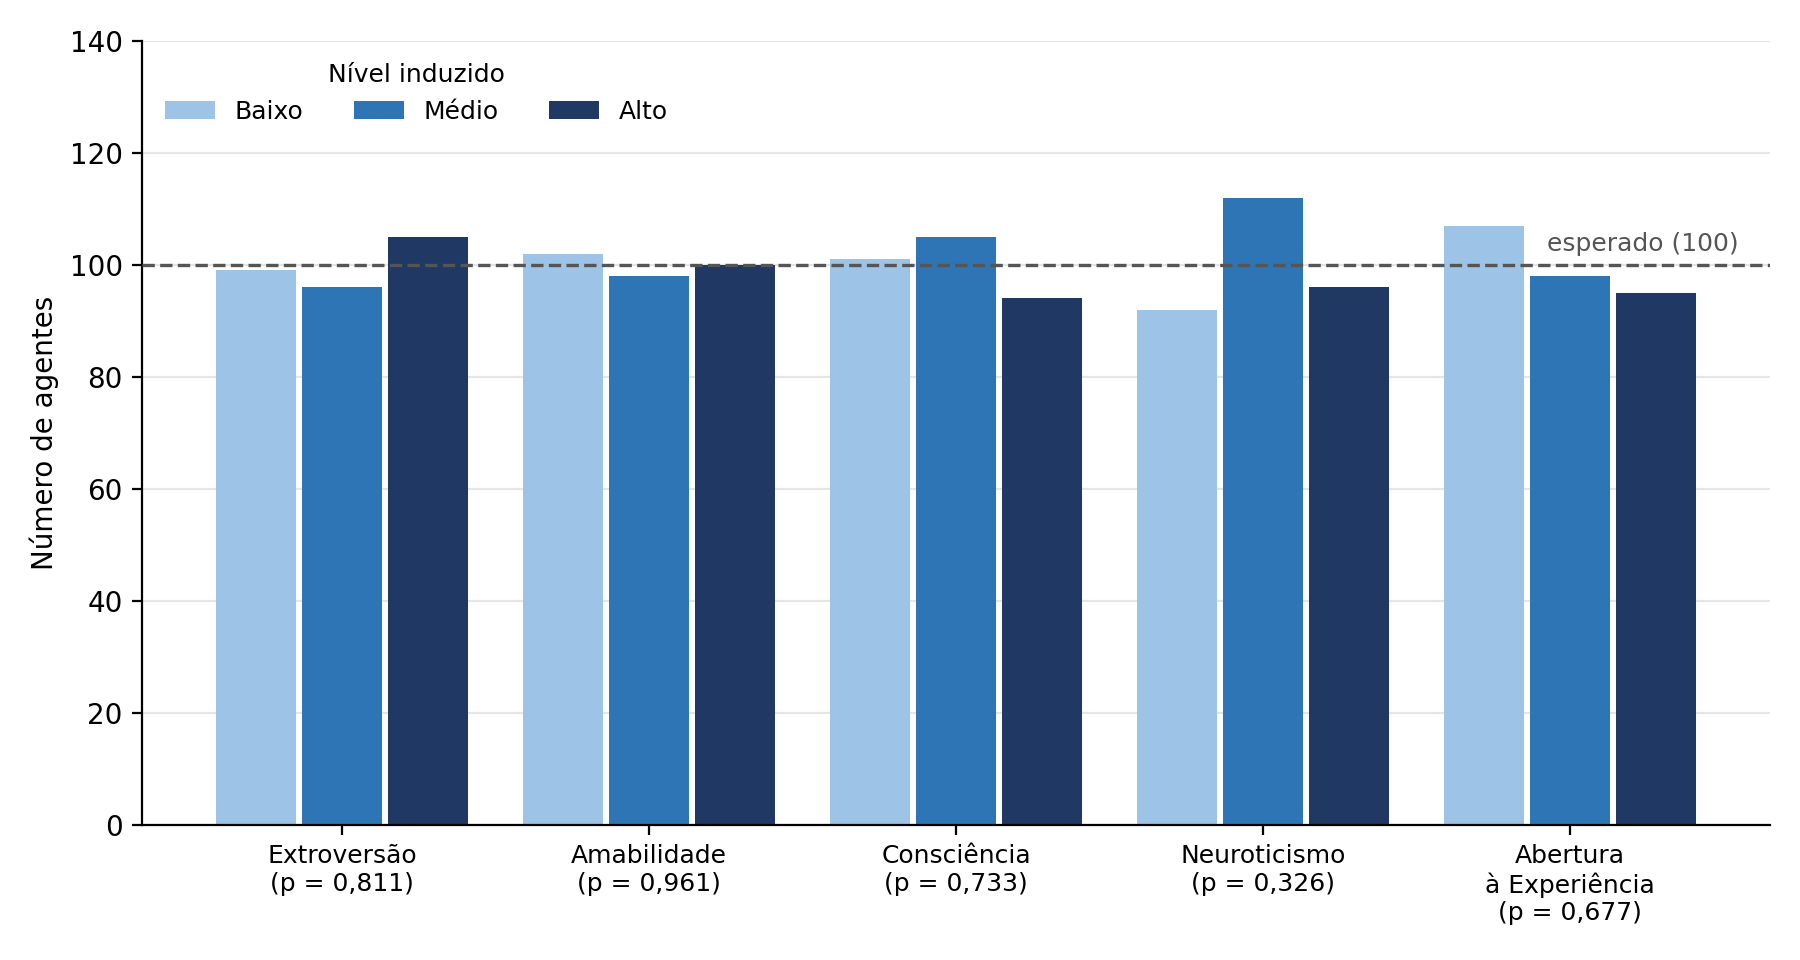
\includegraphics[width=\textwidth]{../resultados/figuras/fig10_aleatorizacao_niveis.png}
    \legend{Fonte: dados da pesquisa. Linha tracejada: contagem esperada em um sorteio uniforme.}
\end{figure}

\subsection{Independência entre os traços}

Nenhum par de traços apresentou associação significativa entre os níveis
sorteados ($|\rho| \leq$ \aleatRhoMax, p $\geq$ \aleatPRhoMin; V de Cramér
$\leq$ \aleatCramerMax; Tabela \ref{tab:aleat-independencia}). Na regressão
OLS com os cinco traços, o fator de inflação da variância ficou entre
\aleatVIFMin{} e \aleatVIFMax, ou seja, sem multicolinearidade entre os
preditores.

% Gerado por analise_aleatorizacao.py -- não editar à mão; rode o script de novo.
\begin{table}[htb]
    \caption{Associação entre os níveis induzidos de cada par de traços (Experimento A)}
    \label{tab:aleat-independencia}
    \centering
    \footnotesize
    \begin{tabular}{lccccc}
        \toprule
        Par de traços & $\rho$ & p ($\rho$) & $\chi^2$ & p ($\chi^2$) & V de Cramér \\
        \midrule
        Amabilidade $\times$ Neuroticismo & +0,103 & 0,075 & 3,50 & 0,478 & 0,076 \\
        Consciência $\times$ Neuroticismo & +0,053 & 0,364 & 1,74 & 0,783 & 0,054 \\
        Extroversão $\times$ Consciência & $-$0,049 & 0,398 & 6,44 & 0,169 & 0,104 \\
        Amabilidade $\times$ Consciência & +0,040 & 0,494 & 1,84 & 0,764 & 0,055 \\
        Extroversão $\times$ Neuroticismo & $-$0,021 & 0,715 & 0,69 & 0,953 & 0,034 \\
        Extroversão $\times$ Amabilidade & +0,015 & 0,790 & 3,81 & 0,433 & 0,080 \\
        Extroversão $\times$ Abertura à Experiência & +0,011 & 0,855 & 2,46 & 0,652 & 0,064 \\
        Amabilidade $\times$ Abertura à Experiência & $-$0,011 & 0,845 & 4,17 & 0,383 & 0,083 \\
        Consciência $\times$ Abertura à Experiência & $-$0,006 & 0,921 & 3,78 & 0,436 & 0,079 \\
        Neuroticismo $\times$ Abertura à Experiência & $-$0,003 & 0,958 & 4,97 & 0,290 & 0,091 \\
        \bottomrule
    \end{tabular}
    \legend{Fonte: dados da pesquisa. $\rho$: correlação de Spearman; $\chi^2$: teste de independência (4 graus de liberdade).}
\end{table}


\subsection{Comparação com sorteios simulados}

Para avaliar se o sorteio obtido é típico do acaso, foram simulados
\aleatNSim{} sorteios com o mesmo desenho. Em todos os indicadores da
Tabela \ref{tab:aleat-montecarlo}, o sorteio obtido ficou dentro da faixa
produzida pelas simulações. O número de combinações distintas de níveis
(\aleatCombUnicas{} das 243 possíveis) é próximo da média simulada
(\aleatCombEsperado); combinações sem nenhum agente são, portanto, uma
propriedade esperada do desenho por sorteio, e não uma falha dele.

% Gerado por analise_aleatorizacao.py -- não editar à mão; rode o script de novo.
\begin{table}[htb]
    \caption{Sorteio obtido vs. 10.000 sorteios simulados}
    \label{tab:aleat-montecarlo}
    \centering
    \footnotesize
    \begin{tabular}{lcc}
        \toprule
        Indicador & Obtido & Simulação \\
        \midrule
        Combinações distintas (de 243 possíveis) & 174 & média 172,4; IC 95\% 163 a 182 \\
        Máximo de agentes com a mesma combinação & 5 & IC 95\% 4 a 7 \\
        Maior $|\rho|$ entre pares de traços & 0,103 & 54,2\% das simulações $\geq$ obtido \\
        Maior desvio de uma contagem em relação a 100 & 12 & 86,9\% das simulações $\geq$ obtido \\
        \bottomrule
    \end{tabular}
    \legend{Fonte: dados da pesquisa. Simulação: 300 agentes, 5 traços, 3 níveis equiprováveis e independentes.}
\end{table}


\subsection{Impacto sobre os resultados}

Se o sorteio tivesse produzido traços correlacionados, o coeficiente de um
traço mudaria ao incluir os demais no modelo. A Tabela
\ref{tab:aleat-impacto} mostra que isso não ocorre: os coeficientes da
regressão simples e da OLS com os cinco traços são muito próximos (Abertura à
Experiência: \aleatAberturaCoefSimples{} e \aleatAberturaCoefMulti), e os
traços significativos são os mesmos nos dois modelos.

% Gerado por analise_aleatorizacao.py -- não editar à mão; rode o script de novo.
\begin{table}[htb]
    \caption{Coeficiente de cada traço sobre o escore IPA: regressão simples vs. OLS com os 5 traços (Experimento A)}
    \label{tab:aleat-impacto}
    \centering
    \small
    \begin{tabular}{lcccc}
        \toprule
        Traço & Coef. simples & p-valor & Coef. OLS (5 traços) & p-valor \\
        \midrule
        Abertura à Experiência & +1,722 & $<$ 0,001 & +1,716 & $<$ 0,001 \\
        Extroversão & +1,165 & $<$ 0,001 & +1,189 & $<$ 0,001 \\
        Consciência & +0,704 & $<$ 0,001 & +0,750 & $<$ 0,001 \\
        Neuroticismo & +0,424 & 0,033 & +0,407 & 0,006 \\
        Amabilidade & +0,164 & 0,392 & +0,094 & 0,511 \\
        \bottomrule
    \end{tabular}
    \legend{Fonte: dados da pesquisa. Variável dependente: escore IPA sem a pergunta 1 (N=300).}
\end{table}


\subsection{Experimento B e pergunta 1 do IPA}

No Experimento B, o traço dominante foi distribuído de forma equilibrada
entre os agentes ($\chi^2$ = \aleatDominanteChi, p = \aleatDominanteP;
Tabela \ref{tab:aleat-exp-b}). O único desequilíbrio está nos níveis de
Neuroticismo quando dominante (p = \aleatNeuroBP), que deixa de ser
significativo após a correção de Bonferroni para os cinco testes (limite
de 0,01). Esse desequilíbrio pode reduzir ligeiramente o poder do teste
de Neuroticismo isolado.

% Gerado por analise_aleatorizacao.py -- não editar à mão; rode o script de novo.
\begin{table}[htb]
    \caption{Distribuição do traço dominante e de seus níveis (Experimento B)}
    \label{tab:aleat-exp-b}
    \centering
    \small
    \begin{tabular}{lccccc}
        \toprule
        Traço dominante & N & Baixo & Médio & Alto & p-valor \\
        \midrule
        Neuroticismo & 69 & 21 & 15 & 33 & 0,026 \\
        Consciência & 63 & 19 & 25 & 19 & 0,565 \\
        Amabilidade & 62 & 21 & 16 & 25 & 0,374 \\
        Extroversão & 57 & 22 & 22 & 13 & 0,241 \\
        Abertura à Experiência & 49 & 13 & 20 & 16 & 0,470 \\
        \bottomrule
    \end{tabular}
    \legend{Fonte: dados da pesquisa. p-valor: qui-quadrado de aderência à uniforme entre os 3 níveis. Distribuição do traço dominante: $\chi^2$ = 3,73, p = 0,443.}
\end{table}


A pergunta 1 do IPA (faixa etária), também sorteada, não se afastou da
distribuição uniforme no Experimento A ($\chi^2$ = \aleatQUmChi, p =
\aleatQUmP). Como as análises usam o escore IPA sem essa pergunta, ela não
interfere nos resultados.

\section{Estudo piloto (BFI-10)}
\label{sec:resultados-piloto}

A Tabela \ref{tab:manipulacao-piloto} e a Figura \ref{fig:manipulacao-piloto}
apresentam a checagem de manipulação do estudo piloto: correlação de
Spearman entre o nível de personalidade induzido (1/2/3) e o escore de
autorrelato do agente no BFI-10, por traço.

\begin{table}[htb]
    \caption{Estudo piloto: correlação entre nível induzido e autorrelato (BFI-10, N=300)}
    \label{tab:manipulacao-piloto}
    \centering
    \begin{tabular}{lccc}
        \toprule
        Traço & $\rho$ & p-valor & Avaliação \\
        \midrule
        Neuroticismo            & 0,838 & $<$ 0,001 & Forte \\
        Amabilidade              & 0,812 & $<$ 0,001 & Forte \\
        Abertura à Experiência  & 0,739 & $<$ 0,001 & Forte \\
        Consciência             & 0,507 & $<$ 0,001 & Forte \\
        Extroversão             & 0,410 & $<$ 0,001 & Moderada \\
        \bottomrule
    \end{tabular}
    \legend{Fonte: dados da pesquisa. Avaliação: forte para $\rho \geq 0{,}50$; moderada para $0{,}30 \leq \rho < 0{,}50$.}
\end{table}

\begin{figure}[htb]
    \caption{Estudo piloto: checagem de manipulação por traço (BFI-10)}
    \label{fig:manipulacao-piloto}
    \centering
    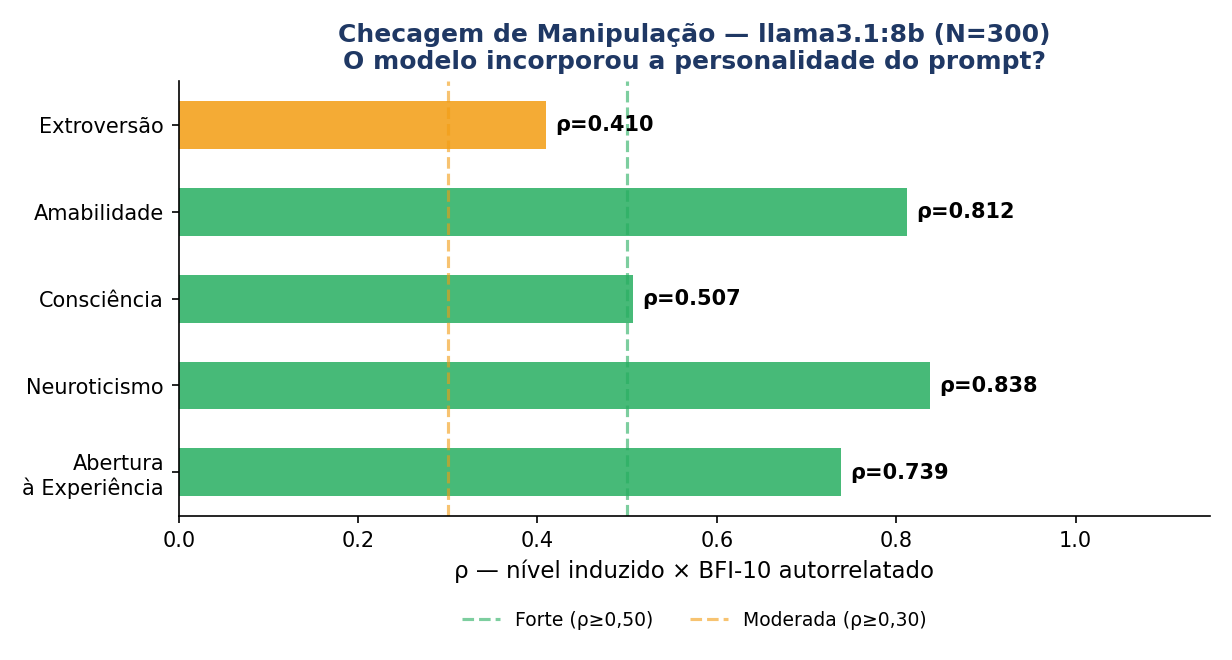
\includegraphics[width=0.8\textwidth]{../resultados/figuras/fig4_manipulacao_piloto.png}
    \legend{Fonte: dados da pesquisa.}
\end{figure}

Todos os cinco traços foram incorporados de forma estatisticamente
significativa; Extroversão foi a mais fraca (ainda assim moderada),
padrão compatível com o viés de discordância em itens de pontuação
reversa descrito na seção \ref{sec:limitacoes-pipeline}.

A Tabela \ref{tab:distribuicao-ipa-piloto} mostra a distribuição do
perfil de investidor obtido, e a Tabela \ref{tab:spearman-ipa-piloto}
(com as Figuras \ref{fig:spearman-piloto} e \ref{fig:boxplots-piloto}) a
correlação entre nível induzido e escore do IPA, por traço.

\begin{table}[htb]
    \caption{Estudo piloto: distribuição do perfil IPA (BFI-10, N=300)}
    \label{tab:distribuicao-ipa-piloto}
    \centering
    \begin{tabular}{lcc}
        \toprule
        Perfil & N & \% \\
        \midrule
        Conservador & 15  & 5\%  \\
        Moderado    & 235 & 78\% \\
        Arrojado    & 50  & 17\% \\
        \bottomrule
    \end{tabular}
    \legend{Fonte: dados da pesquisa. Escore IPA (Q2--Q8): média = 17,83; desvio padrão = 2,74.}
\end{table}

\begin{table}[htb]
    \caption{Estudo piloto: correlação de Spearman entre nível induzido e escore IPA (BFI-10, N=300)}
    \label{tab:spearman-ipa-piloto}
    \centering
    \begin{tabular}{lcc}
        \toprule
        Traço & $\rho$ & p-valor \\
        \midrule
        Abertura à Experiência & 0,326 & $<$ 0,001 \\
        Extroversão            & 0,221 & $<$ 0,001 \\
        Amabilidade             & 0,083 & 0,152 \\
        Neuroticismo           & 0,044 & 0,449 \\
        Consciência            & 0,013 & 0,821 \\
        \bottomrule
    \end{tabular}
    \legend{Fonte: dados da pesquisa.}
\end{table}

\begin{figure}[htb]
    \caption{Estudo piloto: correlação de Spearman entre nível induzido e escore IPA}
    \label{fig:spearman-piloto}
    \centering
    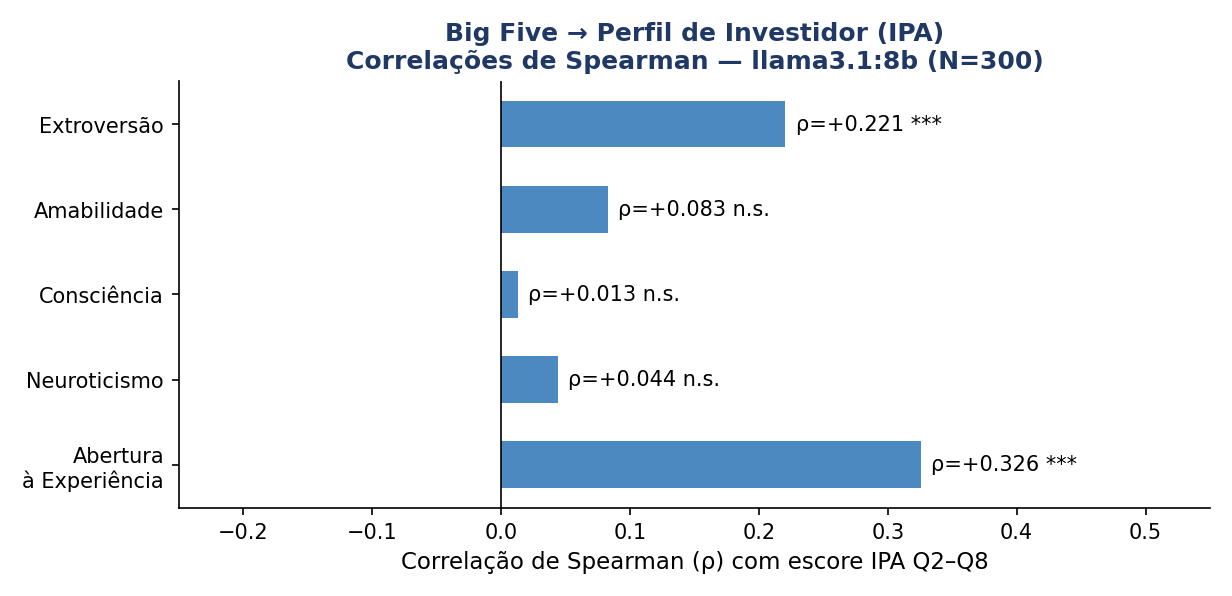
\includegraphics[width=0.8\textwidth]{../resultados/figuras/fig1_spearman_piloto.png}
    \legend{Fonte: dados da pesquisa.}
\end{figure}

\begin{figure}[htb]
    \caption{Estudo piloto: distribuição do escore IPA por nível induzido (\textit{boxplots})}
    \label{fig:boxplots-piloto}
    \centering
    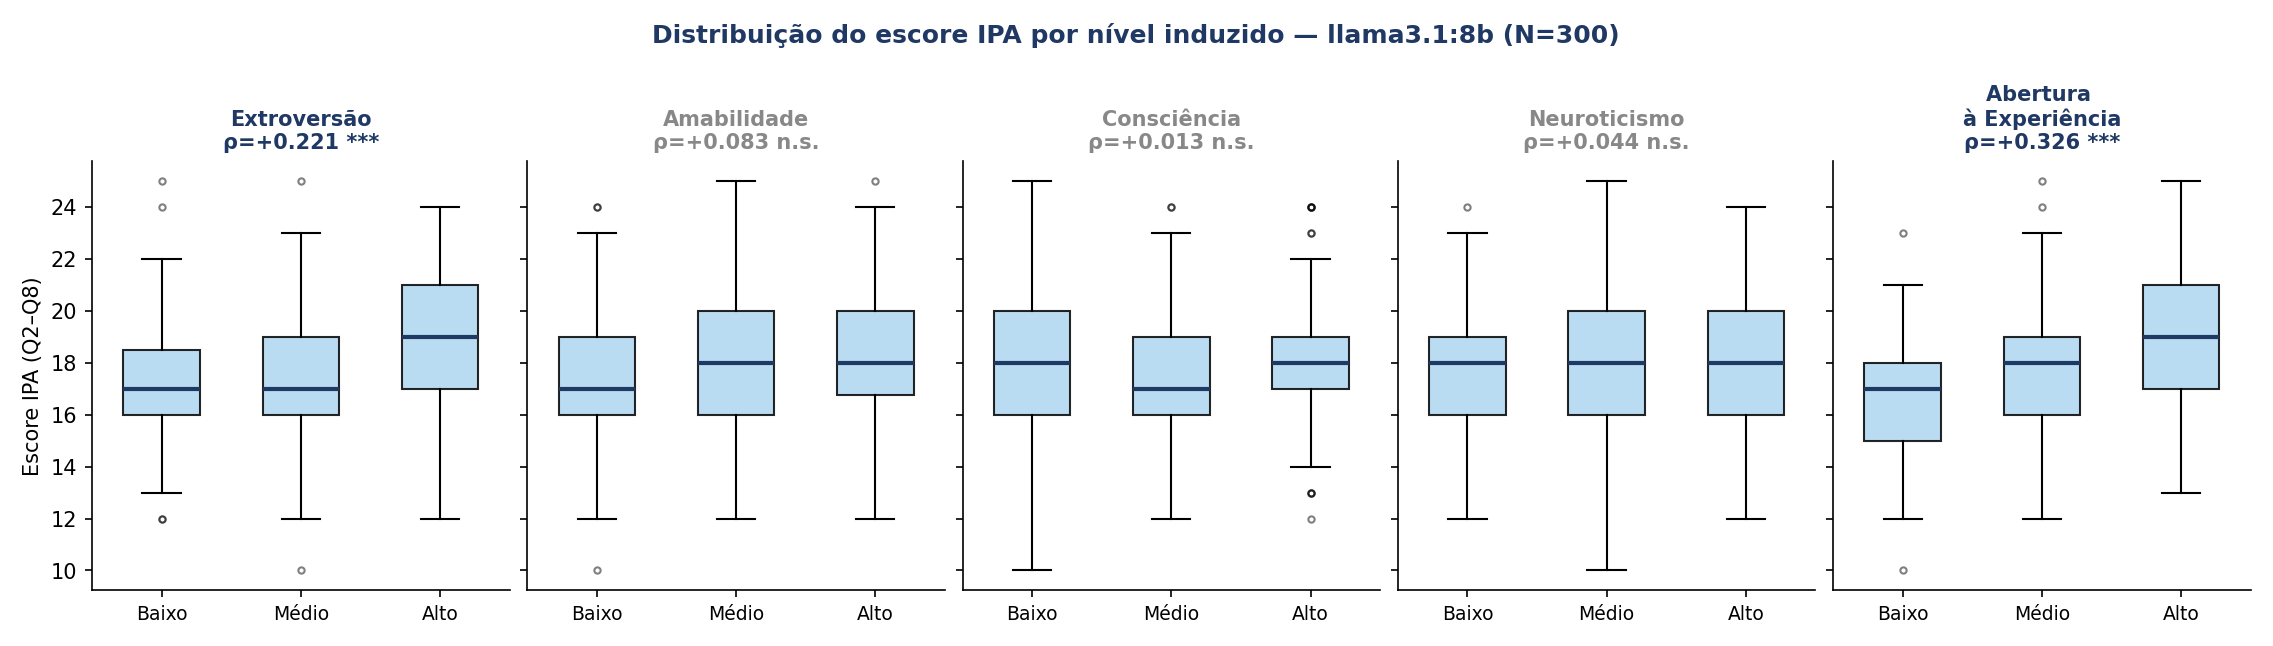
\includegraphics[width=\textwidth]{../resultados/figuras/fig2_boxplots_piloto.png}
    \legend{Fonte: dados da pesquisa.}
\end{figure}

Na regressão OLS com os cinco traços simultâneos (Tabela
\ref{tab:ols-piloto}, Figura \ref{fig:ols-piloto}), o modelo geral obteve
$R^2=0{,}169$; $F(5, 294)=11{,}96$; $p<0{,}001$. Apenas Abertura à
Experiência e Extroversão apresentaram coeficiente estatisticamente
significativo.

\begin{table}[htb]
    \caption{Estudo piloto: regressão OLS, variável dependente: escore IPA (BFI-10, Q2--Q8)}
    \label{tab:ols-piloto}
    \centering
    \begin{tabular}{lcc}
        \toprule
        Traço & Coeficiente & p-valor \\
        \midrule
        Abertura à Experiência & 1,117 & $<$ 0,001 \\
        Extroversão            & 0,717 & $<$ 0,001 \\
        Amabilidade             & 0,261 & 0,145 \\
        Neuroticismo           & 0,179 & 0,335 \\
        Consciência            & 0,069 & 0,705 \\
        \bottomrule
    \end{tabular}
    \legend{Fonte: dados da pesquisa.}
\end{table}

\begin{figure}[htb]
    \caption{Estudo piloto: coeficientes da regressão OLS por traço}
    \label{fig:ols-piloto}
    \centering
    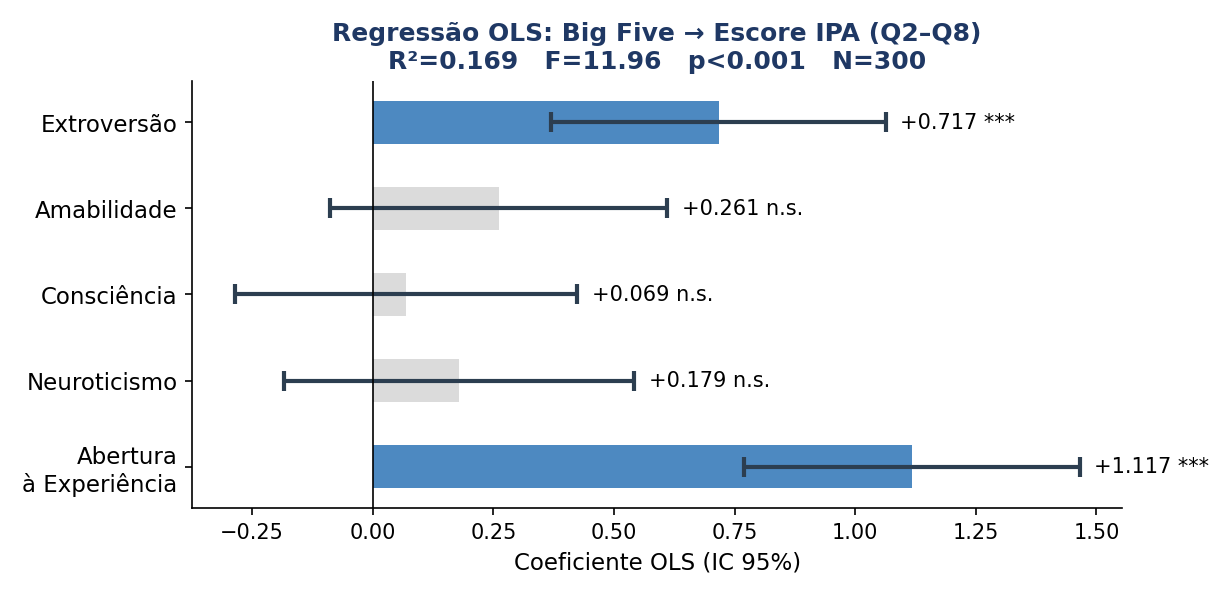
\includegraphics[width=0.8\textwidth]{../resultados/figuras/fig3_ols_piloto.png}
    \legend{Fonte: dados da pesquisa.}
\end{figure}

Esses resultados motivaram tanto a escolha do \texttt{llama3.1:8b} como
modelo principal (seção \ref{sec:selecao-modelo}) quanto a migração para
o BFI-44 como instrumento de checagem de manipulação na análise
principal, reportada a seguir.

\section{Análise principal: Experimento A (BFI-44, multi-traço)}
\label{sec:resultados-exp-a}

\subsection{Checagem de manipulação}
\label{sec:resultados-manipulacao}

A Tabela \ref{tab:manipulacao} apresenta a correlação de Spearman entre o
nível de personalidade induzido (1/2/3) e o escore de autorrelato do
agente no BFI-44, por traço.

\begin{table}[htb]
    \caption{Experimento A: correlação entre nível induzido e autorrelato de personalidade (N=300)}
    \label{tab:manipulacao}
    \centering
    \begin{tabular}{lccc}
        \toprule
        Traço & $\rho$ & p-valor & Avaliação \\
        \midrule
        Extroversão              & 0,929 & $<$ 0,001 & Forte \\
        Abertura à Experiência   & 0,913 & $<$ 0,001 & Forte \\
        Consciência              & 0,879 & $<$ 0,001 & Forte \\
        Neuroticismo             & 0,835 & $<$ 0,001 & Forte \\
        Amabilidade              & 0,813 & $<$ 0,001 & Forte \\
        \bottomrule
    \end{tabular}
    \legend{Fonte: dados da pesquisa.}
\end{table}

\begin{figure}[htb]
    \caption{Experimento A: checagem de manipulação por traço}
    \label{fig:manipulacao}
    \centering
    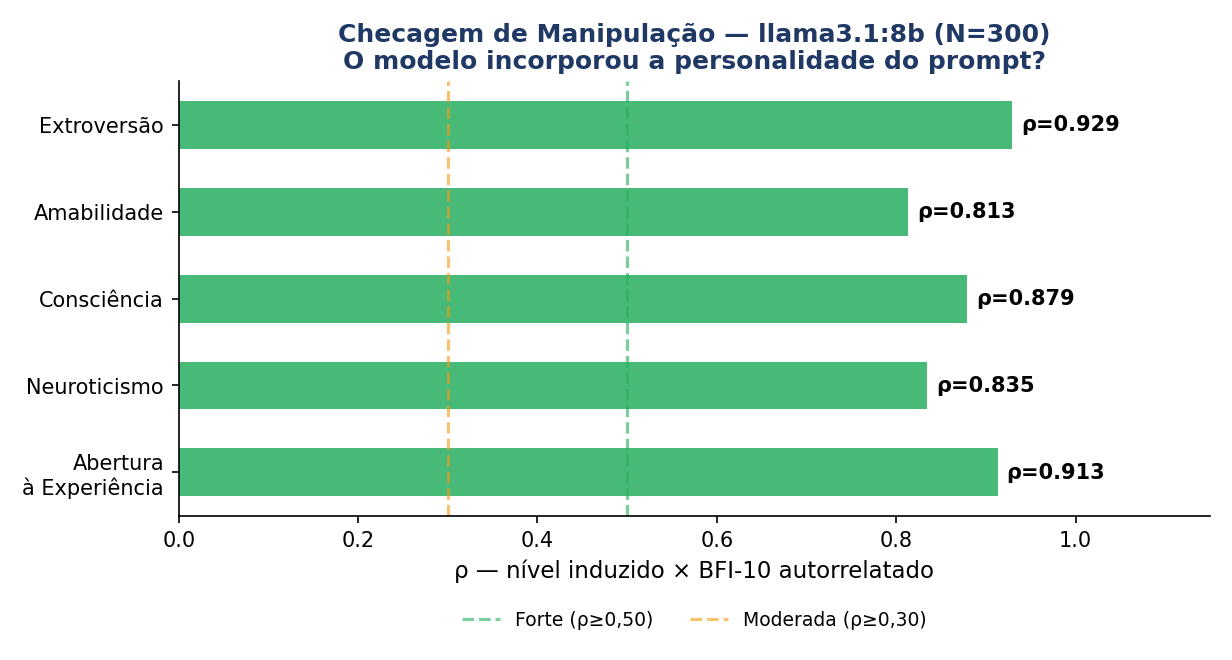
\includegraphics[width=0.8\textwidth]{../resultados/figuras/fig4_manipulacao.png}
    \legend{Fonte: dados da pesquisa.}
\end{figure}

Todos os cinco traços foram incorporados de forma forte e
estatisticamente significativa ($\rho$ de 0,813 a 0,929; Tabela
\ref{tab:manipulacao} e Figura \ref{fig:manipulacao}), uma faixa mais
alta e mais uniforme do que no estudo piloto com BFI-10 (0,410 a 0,838,
Tabela \ref{tab:manipulacao-piloto}).

\subsection{Correlação entre os traços autorrelatados}
\label{sec:resultados-intercorrelacao}

O \texttt{llama3.1:8b} produziu pouca correlação entre os traços
autorrelatados. A
correlação média, em módulo, entre os escores de autorrelato dos 10 pares
de traços foi de 0,110; a maior foi entre Extroversão e Amabilidade
($\rho$ = 0,281), e 4 dos 10 pares tiveram correlação significativa. Como
os níveis induzidos são independentes por construção, essas correlações
vêm do próprio modelo. Mesmo assim, cada nível induzido se reflete
sobretudo no autorrelato do próprio traço: a correlação com o próprio
autorrelato vai de 0,813 a 0,929 (Tabela \ref{tab:manipulacao}), enquanto
a maior correlação entre o nível induzido de um traço e o autorrelato de
outro foi de 0,231 (Amabilidade induzida e Consciência autorrelatada).
Abertura à Experiência foi o traço menos afetado pelos demais: nenhum
outro nível induzido teve correlação significativa com a Abertura
autorrelatada (a maior foi 0,107, com Extroversão; p = 0,063), e incluir
os outros quatro níveis induzidos acrescenta apenas 0,011 ao $R^2$ do
autorrelato de Abertura explicado pelo seu próprio nível. Esse resultado
é compatível com um efeito de Abertura à Experiência sobre o IPA,
reportado a seguir, que não decorre da indução de outro traço.

\subsection{Distribuição do perfil de investidor (IPA)}

A Tabela \ref{tab:distribuicao-ipa} mostra a distribuição do perfil de
investidor obtido no Experimento A.

\begin{table}[htb]
    \caption{Experimento A: distribuição do perfil IPA (N=300)}
    \label{tab:distribuicao-ipa}
    \centering
    \begin{tabular}{lcc}
        \toprule
        Perfil & N & \% \\
        \midrule
        Conservador & 11  & 3,7\%  \\
        Moderado    & 247 & 82,3\% \\
        Arrojado    & 42  & 14,0\% \\
        \bottomrule
    \end{tabular}
    \legend{Fonte: dados da pesquisa. Escore IPA (Q2--Q8): média = 17,58; desvio padrão = 2,72.}
\end{table}

\subsection{Correlação de Spearman: nível induzido \texorpdfstring{$\times$}{x} escore IPA}

A Tabela \ref{tab:spearman-ipa} e as Figuras \ref{fig:spearman} e
\ref{fig:boxplots} apresentam a correlação entre o nível induzido e o
escore do IPA, por traço.

\begin{table}[htb]
    \caption{Experimento A: correlação de Spearman entre nível induzido e escore IPA (N=300)}
    \label{tab:spearman-ipa}
    \centering
    \begin{tabular}{lcc}
        \toprule
        Traço & $\rho$ & p-valor \\
        \midrule
        Abertura à Experiência & 0,530 & $<$ 0,001 \\
        Extroversão            & 0,340 & $<$ 0,001 \\
        Consciência            & 0,206 & $<$ 0,001 \\
        Neuroticismo           & 0,136 & 0,018 \\
        Amabilidade             & 0,051 & 0,376 \\
        \bottomrule
    \end{tabular}
    \legend{Fonte: dados da pesquisa.}
\end{table}

\begin{figure}[htb]
    \caption{Experimento A: correlação de Spearman entre nível induzido e escore IPA}
    \label{fig:spearman}
    \centering
    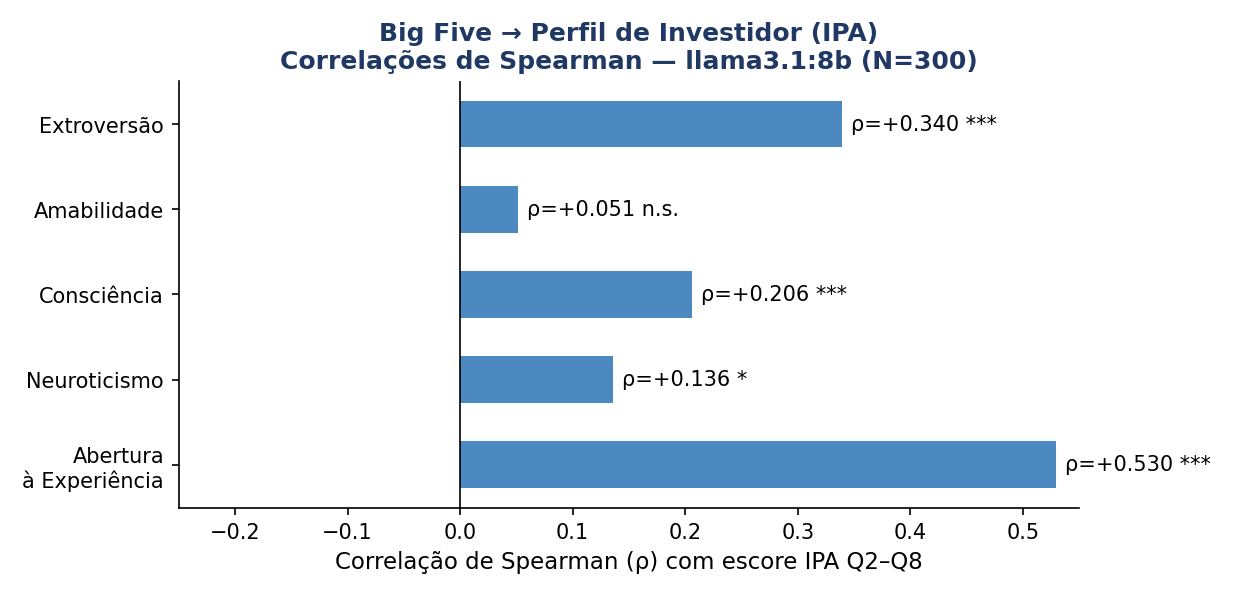
\includegraphics[width=0.8\textwidth]{../resultados/figuras/fig1_spearman.png}
    \legend{Fonte: dados da pesquisa.}
\end{figure}

\begin{figure}[htb]
    \caption{Experimento A: distribuição do escore IPA por nível induzido (\textit{boxplots})}
    \label{fig:boxplots}
    \centering
    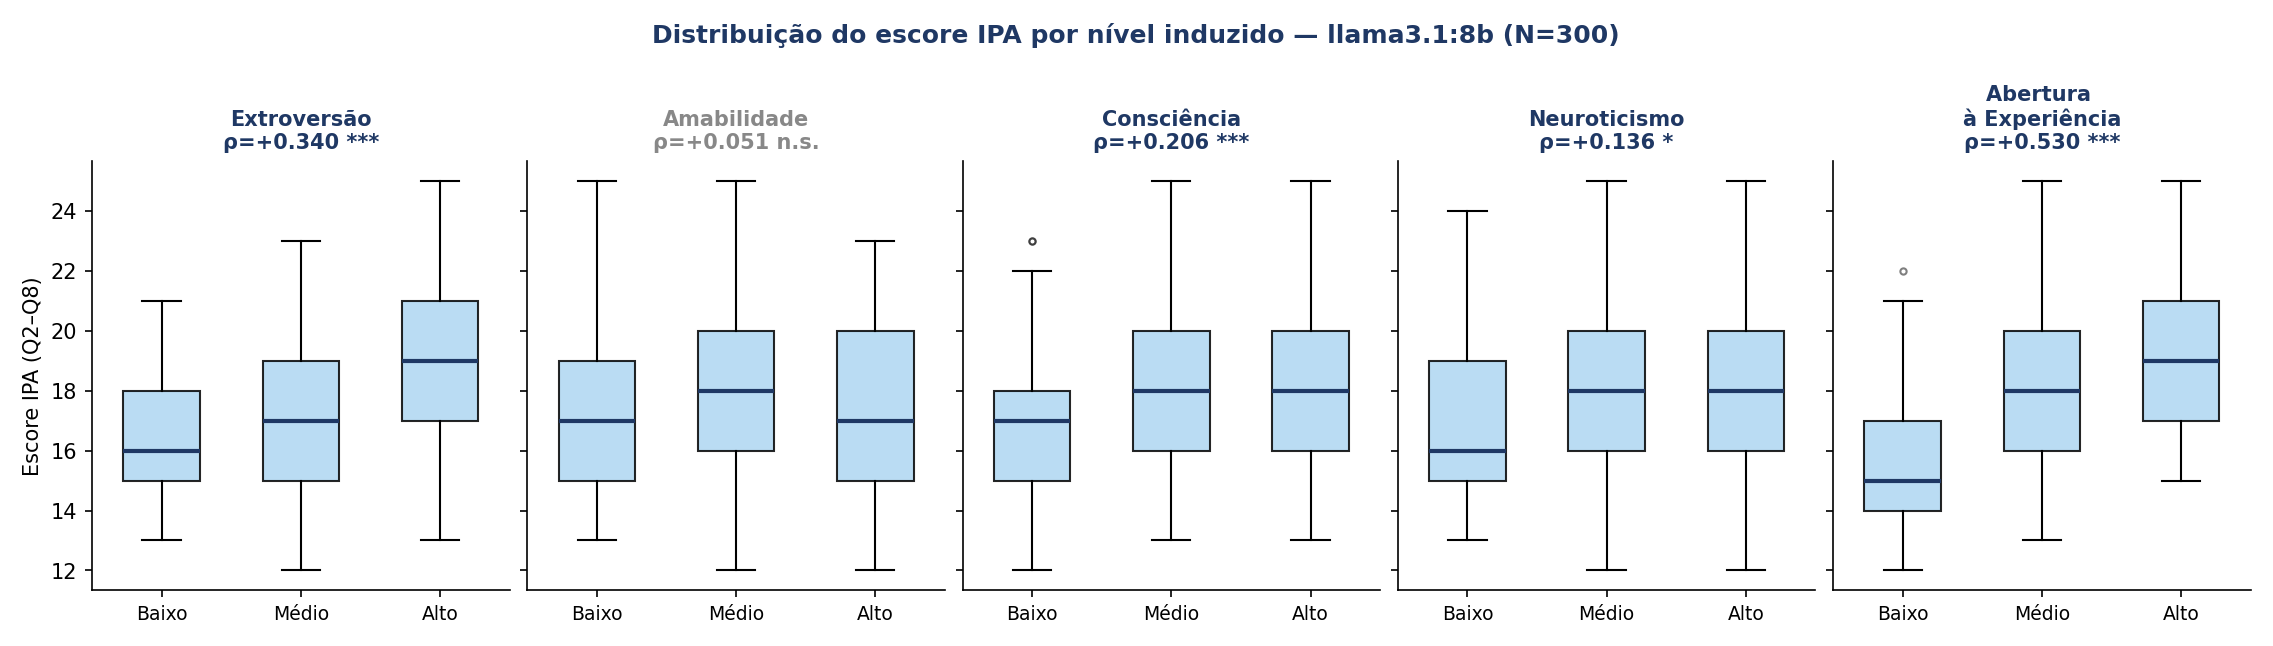
\includegraphics[width=\textwidth]{../resultados/figuras/fig2_boxplots.png}
    \legend{Fonte: dados da pesquisa.}
\end{figure}

\subsection{Regressão OLS com os cinco traços simultâneos}

Os resultados da regressão estão na Tabela \ref{tab:ols} e na Figura
\ref{fig:ols}. Modelo geral: $R^2=0{,}459$; $F(5, 294)=49{,}85$; $p<0{,}001$.

\begin{table}[htb]
    \caption{Experimento A: regressão OLS, variável dependente: escore IPA (Q2--Q8)}
    \label{tab:ols}
    \centering
    \begin{tabular}{lcc}
        \toprule
        Traço & Coeficiente & p-valor \\
        \midrule
        Abertura à Experiência & 1,716 & $<$ 0,001 \\
        Extroversão            & 1,189 & $<$ 0,001 \\
        Consciência            & 0,750 & $<$ 0,001 \\
        Neuroticismo           & 0,407 & 0,006 \\
        Amabilidade             & 0,094 & 0,511 \\
        \bottomrule
    \end{tabular}
    \legend{Fonte: dados da pesquisa.}
\end{table}

\begin{figure}[htb]
    \caption{Experimento A: coeficientes da regressão OLS por traço}
    \label{fig:ols}
    \centering
    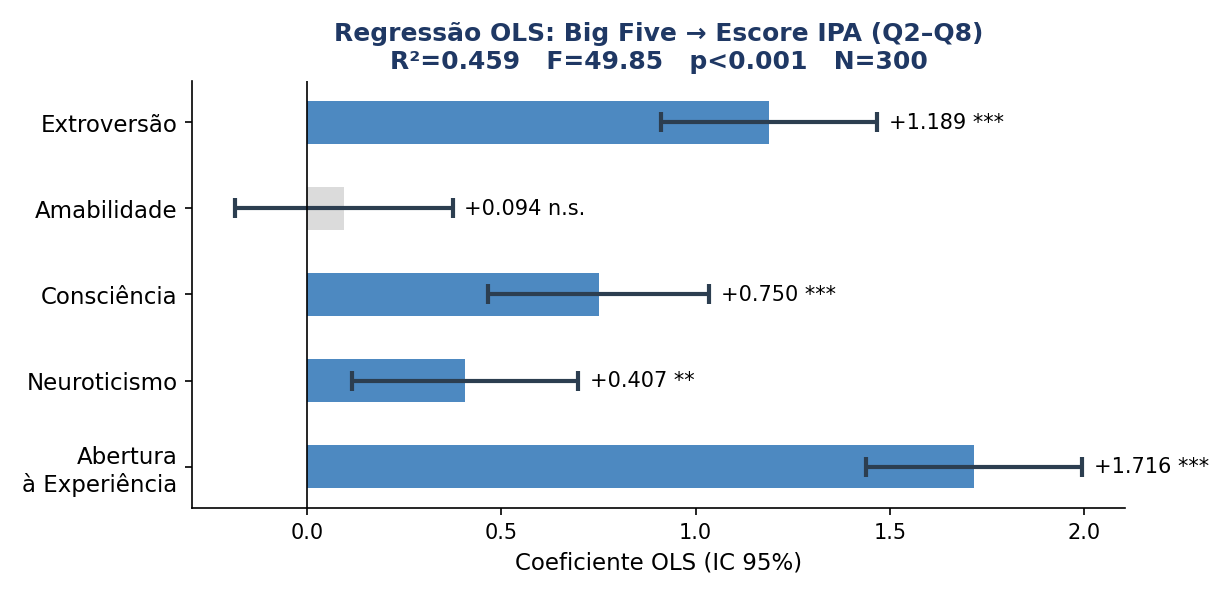
\includegraphics[width=0.8\textwidth]{../resultados/figuras/fig3_ols.png}
    \legend{Fonte: dados da pesquisa.}
\end{figure}

Controlando o efeito dos outros quatro traços, cada passo de nível (de
Baixo para Médio ou de Médio para Alto) em Abertura à Experiência
corresponde, em média, a um acréscimo de 1,716 ponto no escore IPA, o
maior coeficiente entre os cinco traços. Extroversão, Consciência e
Neuroticismo têm coeficientes positivos e estatisticamente significativos
(1,189, 0,750 e 0,407 ponto por passo de nível, respectivamente),
enquanto Amabilidade não apresenta efeito distinguível de zero
(coeficiente de 0,094; $p=0{,}511$). O modelo como um todo explica 45,9\% da variância do
escore IPA, quase o triplo do $R^2$ obtido no estudo piloto com BFI-10
(16,9\%, Tabela \ref{tab:ols-piloto}). Quatro dos cinco traços atingem
significância estatística nesta análise, contra dois no estudo piloto; a
seção seguinte (Experimento B) verifica até que ponto esses quatro
efeitos dependem do desenho de indução simultânea.

\section{Experimento B: traço dominante}
\label{sec:resultados-exp-b}

O Experimento B foi conduzido para verificar se induzir os cinco traços
do Big Five ao mesmo tempo no mesmo agente, como no Experimento A, dilui
ou confunde o sinal de cada traço individual, em comparação com a
indução de apenas um traço por vez. Para testar isso de forma
controlada, o Experimento B usa o mesmo modelo e instrumento do
Experimento A, mudando apenas o desenho de indução: cada agente tem
apenas um dos cinco traços sorteado para variar (o ``traço dominante''),
com os outros quatro fixos em ``Médio'' (a seção \ref{sec:exp-a-b}
descreve o raciocínio metodológico completo; a interpretação dos números
a seguir está no Capítulo \ref{cap:discussao}, seção
\ref{sec:discussao-exp-b}). A Tabela \ref{tab:manipulacao-exp-b} reporta
a checagem de manipulação, calculada apenas entre os agentes em que
aquele traço era o dominante (por isso o N varia por linha, de 49 a 69),
lado a lado com o valor correspondente do Experimento A.

\begin{table}[htb]
    \caption{Checagem de manipulação: Experimento A (todos os traços variando) vs. Experimento B (só o traço dominante variando)}
    \label{tab:manipulacao-exp-b}
    \centering
    \begin{tabular}{lcccc}
        \toprule
        Traço & $\rho$ Exp. A & $\rho$ Exp. B & N (Exp. B) & p-valor (Exp. B) \\
        \midrule
        Extroversão              & 0,929 & 0,930 & 57 & $<$ 0,001 \\
        Abertura à Experiência   & 0,913 & 0,928 & 49 & $<$ 0,001 \\
        Consciência              & 0,879 & 0,896 & 63 & $<$ 0,001 \\
        Neuroticismo             & 0,835 & 0,840 & 69 & $<$ 0,001 \\
        Amabilidade              & 0,813 & 0,837 & 62 & $<$ 0,001 \\
        \bottomrule
    \end{tabular}
    \legend{Fonte: dados da pesquisa. Coluna ``Exp. B'' calculada apenas entre os agentes em que o traço da linha era o traço dominante sorteado.}
\end{table}

\begin{figure}[htb]
    \caption{Checagem de manipulação: Experimento A vs. Experimento B, por traço}
    \label{fig:exp-ab-manipulacao}
    \centering
    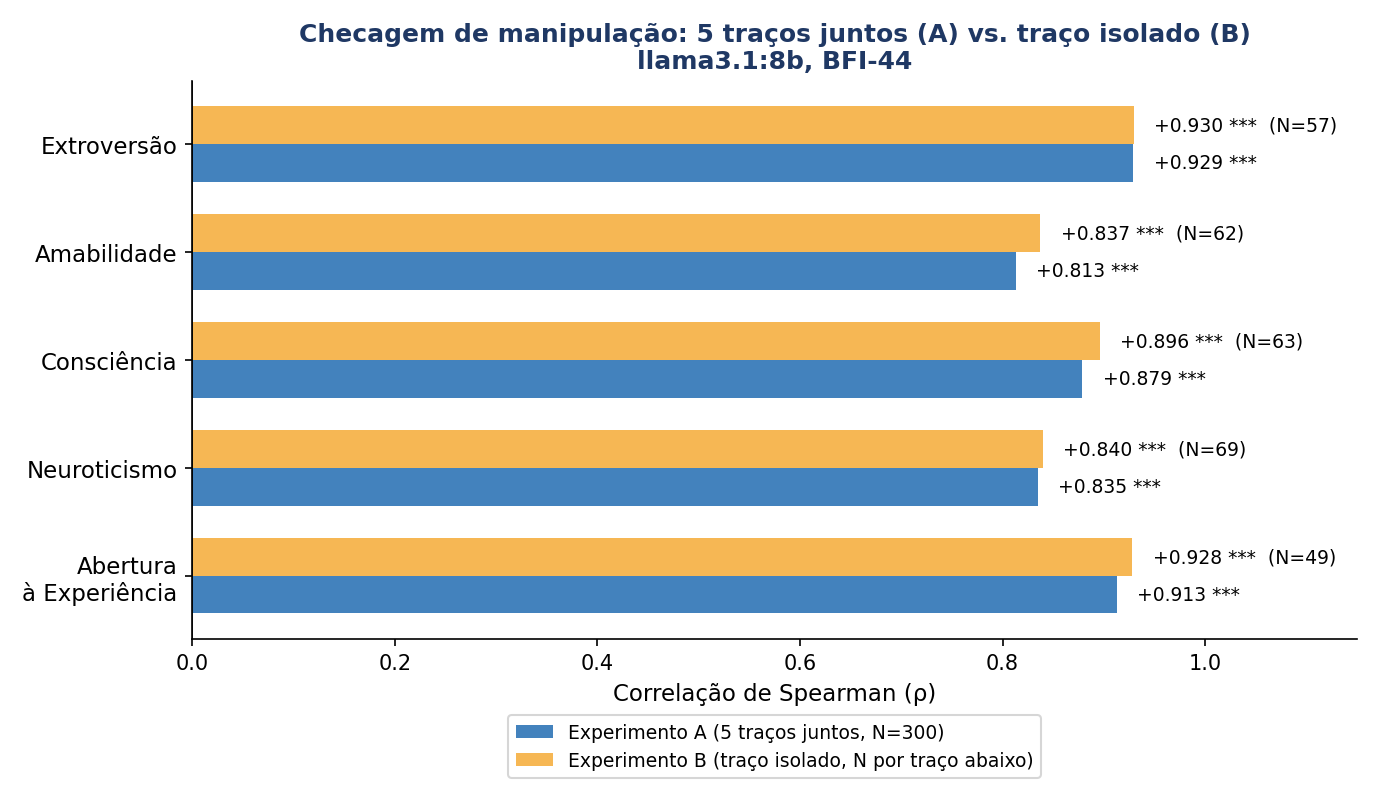
\includegraphics[width=0.85\textwidth]{../resultados/figuras/fig8_exp_ab_manipulacao.png}
    \legend{Fonte: dados da pesquisa.}
\end{figure}

Na Figura \ref{fig:exp-ab-manipulacao}, os valores dos dois experimentos
são praticamente iguais em todos os traços, entre 0,8 e 0,95.

A Tabela \ref{tab:ipa-exp-b} reporta a correlação entre nível induzido e
escore do IPA, na mesma estratificação, lado a lado com o Experimento A.

\begin{table}[htb]
    \caption{Correlação com o escore IPA: Experimento A (todos os traços) vs. Experimento B (traço dominante)}
    \label{tab:ipa-exp-b}
    \centering
    \begin{tabular}{lcccc}
        \toprule
        Traço & $\rho$ Exp. A & $\rho$ Exp. B & N (Exp. B) & p-valor (Exp. B) \\
        \midrule
        Abertura à Experiência   & 0,530  & 0,792  & 49 & $<$ 0,001 \\
        Extroversão              & 0,340  & 0,242  & 57 & 0,070 \\
        Consciência              & 0,206  & 0,153  & 63 & 0,232 \\
        Neuroticismo             & 0,136  & $-$0,116 & 69 & 0,344 \\
        Amabilidade              & 0,051  & $-$0,006 & 62 & 0,966 \\
        \bottomrule
    \end{tabular}
    \legend{Fonte: dados da pesquisa. Coluna ``Exp. B'' calculada apenas entre os agentes em que o traço da linha era o traço dominante sorteado.}
\end{table}

\begin{figure}[htb]
    \caption{Correlação com o escore IPA: Experimento A vs. Experimento B, por traço}
    \label{fig:exp-ab-ipa}
    \centering
    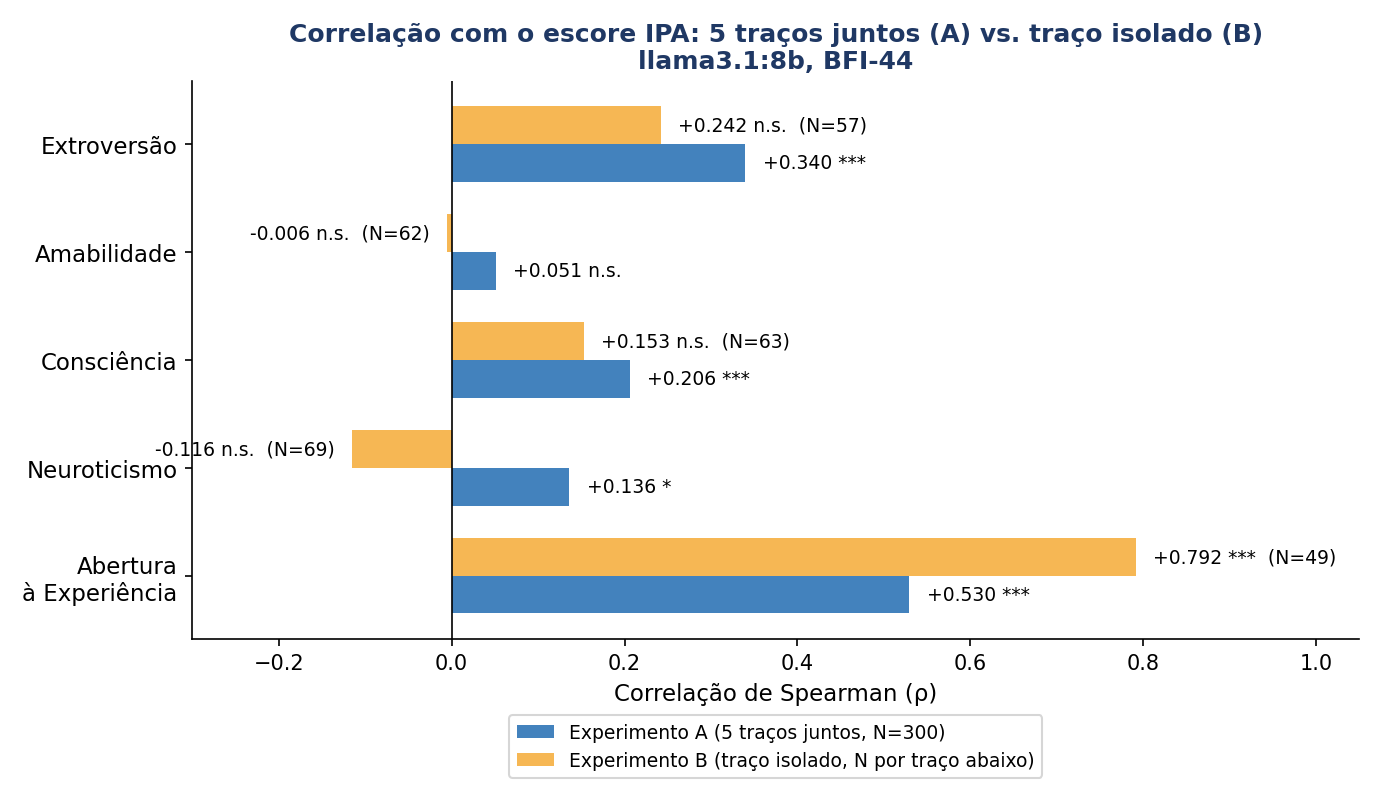
\includegraphics[width=0.85\textwidth]{../resultados/figuras/fig9_exp_ab_ipa.png}
    \legend{Fonte: dados da pesquisa.}
\end{figure}

Ao contrário da Figura \ref{fig:exp-ab-manipulacao}, na Figura
\ref{fig:exp-ab-ipa} os valores dos dois experimentos não são
parecidos em todos os traços: em Abertura à Experiência, a correlação é
maior no Experimento B; nos outros quatro traços, é menor no Experimento
B, e em Neuroticismo e Amabilidade passa a ser negativa.

A checagem de manipulação (Tabela \ref{tab:manipulacao-exp-b}) é
comparável entre os dois desenhos em todos os cinco traços, sem indício
de que a indução simultânea enfraqueça a manipulação. Já a correlação
com o escore IPA (Tabela \ref{tab:ipa-exp-b}) mostra um padrão diferente
por traço: Abertura à Experiência permanece significativa e com
correlação mais alta no Experimento B ($\rho=0{,}792$ contra 0,530); os
outros quatro traços não atingem significância estatística no
Experimento B, com Neuroticismo e Amabilidade invertendo o sinal
(positivo no Experimento A, negativo no B). A interpretação desse
padrão, incluindo o papel do N bem menor por traço no Experimento B
(49 a 69, contra 300 no Experimento A), é discutida no Capítulo
\ref{cap:discussao}.

\section{Análise de robustez e generalização}
\label{sec:resultados-robustez}

Esta seção reporta as repetições do Experimento A descritas na seção
\ref{sec:metodo-robustez}. Em todas as tabelas, o escore IPA é o das
perguntas 2 a 8 e os coeficientes são os da regressão OLS com os cinco
níveis induzidos, com a mesma notação de significância usada no restante
do trabalho (* $p<0{,}05$; ** $p<0{,}01$; *** $p<0{,}001$; n.s. para
$p \geq 0{,}05$). A faixa de manipulação é o menor e o maior $\rho$ entre
nível induzido e autorrelato (BFI-44) entre os cinco traços.

\subsection{Sensibilidade à temperatura}

As três novas rodadas foram concluídas com 300 agentes cada, com BFI-44 válido em
todos e IPA válido em 299 (temperaturas 0,0 e 0,3) e 300 (temperatura
1,0) agentes. A Tabela \ref{tab:robustez-temperatura} compara as quatro
temperaturas.

\begin{table}[htb]
    \caption{Experimento A em quatro temperaturas (\texttt{llama3.1:8b}, N=300, mesmos perfis)}
    \label{tab:robustez-temperatura}
    \centering
    \footnotesize
    \setlength{\tabcolsep}{4pt}
    \begin{tabular}{>{\raggedright\arraybackslash}p{3.4cm}cccc}
        \toprule
        Indicador & 0,0 & 0,3 & 0,7 (Exp. A) & 1,0 \\
        \midrule
        Perfis IPA: Conservador / Moderado / Arrojado (\%) & 2,0 / 86,6 / 11,4 & 3,7 / 84,9 / 11,4 & 3,7 / 82,3 / 14,0 & 4,0 / 81,0 / 15,0 \\
        Escore IPA: média (desvio padrão) & 17,05 (2,41) & 17,09 (2,47) & 17,58 (2,72) & 17,67 (2,77) \\
        Manipulação: faixa de $\rho$ & 0,873 a 0,946 & 0,859 a 0,938 & 0,813 a 0,929 & 0,809 a 0,920 \\
        $R^2$ da regressão OLS & 0,707 & 0,643 & 0,459 & 0,449 \\
        \midrule
        Coef. Abertura à Experiência & 1,767*** & 1,932*** & 1,716*** & 1,686*** \\
        Coef. Extroversão & 1,595*** & 1,273*** & 1,189*** & 1,253*** \\
        Coef. Consciência & 0,429*** & 0,486*** & 0,750*** & 0,301* \\
        Coef. Neuroticismo & 0,419*** & 0,278* & 0,407** & 0,744*** \\
        Coef. Amabilidade & 0,359*** & 0,344** & 0,094 n.s. & 0,246 n.s. \\
        \bottomrule
    \end{tabular}
    \legend{Fonte: dados da pesquisa.}
\end{table}

Abertura à Experiência teve o maior coeficiente nas quatro temperaturas
(de 1,686 a 1,932), sempre com $p<0{,}001$, e Extroversão o segundo maior
(de 1,189 a 1,595), também sempre com $p<0{,}001$. Abaixo de 0,7, a
manipulação fica mais fiel e o $R^2$ sobe (0,643 em 0,3 e 0,707 em 0,0), enquanto em 1,0 o resultado fica
próximo do obtido em 0,7 ($R^2=0{,}449$). Os três traços de efeito menor
oscilam entre temperaturas: o coeficiente de Consciência vai de 0,301
(1,0) a 0,750 (0,7), o de Neuroticismo vai de 0,278 (0,3) a 0,744 (1,0),
e Amabilidade só é significativa em 0,0 e 0,3.

A temperatura 0,0 não tornou a geração totalmente determinística. Como a
pergunta 1 do IPA não entra no \textit{prompt}, agentes com a mesma
combinação de níveis recebem \textit{prompts} idênticos. Entre as 87
combinações de níveis que aparecem em mais de um agente, o escore IPA foi
idêntico em todos os agentes da combinação em 87,4\% delas com
temperatura 0,0, contra 6,9\% com temperatura 0,7.

Como os perfis são os mesmos do Experimento A, cada agente pode ser
comparado consigo mesmo entre temperaturas (Tabela
\ref{tab:robustez-temperatura-pareada}). O mesmo agente recebeu o mesmo
perfil de investidor em 77,3\% a 82,9\% dos casos, com a menor
concordância na temperatura 1,0.

\begin{table}[htb]
    \caption{Comparação agente a agente com o Experimento A (temperatura 0,7)}
    \label{tab:robustez-temperatura-pareada}
    \centering
    \begin{tabular}{lccc}
        \toprule
        Temperatura & Pares & $\rho$ do escore IPA & Mesmo perfil IPA (\%) \\
        \midrule
        0,0 & 299 & 0,620*** & 82,9 \\
        0,3 & 299 & 0,583*** & 82,9 \\
        1,0 & 300 & 0,526*** & 77,3 \\
        \bottomrule
    \end{tabular}
    \legend{Fonte: dados da pesquisa.}
\end{table}

\subsection{Novo sorteio de perfis}

O novo sorteio (semente 456) também ficou equilibrado: cada nível de cada
traço recebeu entre 88 e 117 dos 300 agentes, sem desvio significativo da
distribuição uniforme ($\chi^2$, p $\geq$ 0,101), e os níveis sorteados
ficaram independentes entre os traços ($|\rho| \leq$ 0,087). O BFI-44 foi
válido nos 300 agentes e o IPA em 298. A Tabela \ref{tab:robustez-seed}
compara os dois sorteios.

\begin{table}[htb]
    \caption{Experimento A com dois sorteios de perfis (\texttt{llama3.1:8b}, temperatura 0,7)}
    \label{tab:robustez-seed}
    \centering
    \begin{tabular}{lcc}
        \toprule
        Indicador & Semente 123 (Exp. A) & Semente 456 \\
        \midrule
        Perfis IPA: C / M / A (\%) & 3,7 / 82,3 / 14,0 & 6,7 / 80,2 / 13,1 \\
        Escore IPA: média (desvio padrão) & 17,58 (2,72) & 17,50 (2,77) \\
        Manipulação: faixa de $\rho$ & 0,813 a 0,929 & 0,823 a 0,928 \\
        $R^2$ da regressão OLS & 0,459 & 0,526 \\
        \midrule
        Coef. Abertura à Experiência & 1,716*** & 2,106*** \\
        Coef. Extroversão & 1,189*** & 1,293*** \\
        Coef. Consciência & 0,750*** & 0,048 n.s. \\
        Coef. Neuroticismo & 0,407** & $-$0,092 n.s. \\
        Coef. Amabilidade & 0,094 n.s. & 0,169 n.s. \\
        \bottomrule
    \end{tabular}
    \legend{Fonte: dados da pesquisa. C = Conservador; M = Moderado; A = Arrojado.}
\end{table}

Abertura à Experiência e Extroversão se repetem no novo sorteio, com
coeficientes de tamanho semelhante ou maior (2,106 e 1,293). Consciência
e Neuroticismo, significativos no Experimento A, ficam próximos de zero e
sem significância com outro sorteio de perfis, e Amabilidade continua sem
efeito.

\subsection{Outros modelos de linguagem}

As rodadas com os três modelos abertos foram concluídas com 300 agentes cada, com
os mesmos perfis do Experimento A. A taxa de respostas válidas variou
entre os modelos: o \texttt{gemma3:12b} teve BFI-44 e IPA válidos nos 300
agentes; o \texttt{mistral:7b}, BFI-44 válido em 294 e IPA em 300; e o
\texttt{qwen2.5:7b}, BFI-44 válido em 286 e IPA em 257, de modo que a
análise desse modelo usa os 245 agentes com os dois questionários
válidos. A Tabela \ref{tab:robustez-modelos} reporta os resultados.

\begin{table}[htb]
    \caption{Experimento A em quatro modelos abertos (temperatura 0,7, mesmos perfis)}
    \label{tab:robustez-modelos}
    \centering
    \footnotesize
    \setlength{\tabcolsep}{4pt}
    \begin{tabular}{>{\raggedright\arraybackslash}p{3.3cm}>{\centering\arraybackslash}p{2.5cm}>{\centering\arraybackslash}p{2.5cm}>{\centering\arraybackslash}p{2.5cm}>{\centering\arraybackslash}p{2.5cm}}
        \toprule
        Indicador & \texttt{llama3.1:8b} (Exp. A) & \texttt{qwen2.5:7b} & \texttt{mistral:7b} & \texttt{gemma3:12b} \\
        \midrule
        Agentes na análise & 300 & 245 & 294 & 300 \\
        Perfis IPA: C / M / A (\%) & 3,7 / 82,3 / 14,0 & 4,5 / 51,0 / 44,5 & 0,0 / 8,5 / 91,5 & 24,0 / 59,3 / 16,7 \\
        Escore IPA: média (desvio padrão) & 17,58 (2,72) & 19,48 (4,34) & 22,86 (1,11) & 15,77 (3,89) \\
        Manipulação: faixa de $\rho$ & 0,813 a 0,929 & 0,846 a 0,914 & 0,872 a 0,939 & 0,943 a 0,957 \\
        $R^2$ da regressão OLS & 0,459 & 0,796 & 0,383 & 0,648 \\
        \midrule
        Coef. Abertura à Experiência & 1,716*** & 4,643*** & 0,632*** & 2,622*** \\
        Coef. Extroversão & 1,189*** & 1,551*** & 0,391*** & 2,697*** \\
        Coef. Consciência & 0,750*** & $-$0,426** & 0,034 n.s. & 0,534** \\
        Coef. Neuroticismo & 0,407** & 0,322* & 0,285*** & $-$0,125 n.s. \\
        Coef. Amabilidade & 0,094 n.s. & $-$0,317* & $-$0,287*** & $-$0,193 n.s. \\
        \bottomrule
    \end{tabular}
    \legend{Fonte: dados da pesquisa. C = Conservador; M = Moderado; A = Arrojado.}
\end{table}

A indução de personalidade funcionou nos quatro modelos: nos três
modelos adicionais, o menor $\rho$ de manipulação entre os cinco traços
(0,846 a 0,943) ficou acima do menor $\rho$ do \texttt{llama3.1:8b}
(0,813). Abertura à
Experiência e Extroversão elevam o escore IPA nos quatro, sempre com
$p<0{,}001$, embora o tamanho do efeito varie bastante: no
\texttt{qwen2.5:7b}, o coeficiente de Abertura é cerca de 2,7 vezes o do
\texttt{llama3.1:8b} (4,643 contra 1,716), e no \texttt{mistral:7b} é bem
menor (0,632). Os outros três traços não se repetem: Consciência é
positiva no \texttt{llama3.1:8b} e no \texttt{gemma3:12b}, negativa no
\texttt{qwen2.5:7b} e nula no \texttt{mistral:7b}; Neuroticismo é
positivo em três modelos e nulo no \texttt{gemma3:12b}; e Amabilidade,
nula no \texttt{llama3.1:8b}, é negativa e significativa no
\texttt{qwen2.5:7b} e no \texttt{mistral:7b}.

A distribuição dos perfis de investidor, por sua vez, depende fortemente do modelo.
O \texttt{mistral:7b} classificou 91,5\% dos agentes como Arrojado, com
escore pouco variável (desvio padrão de 1,11), enquanto o
\texttt{llama3.1:8b} classificou 82,3\% como Moderado e o
\texttt{gemma3:12b} teve a maior proporção de Conservadores (24,0\%). A
comparação agente a agente com o \texttt{llama3.1:8b} (Tabela
\ref{tab:robustez-modelos-pareada}) mostra que, com o mesmo perfil de
personalidade, o perfil de investidor coincide em 20,3\% a 62,0\% dos
agentes, conforme o modelo.

\begin{table}[htb]
    \caption{Comparação agente a agente com o \texttt{llama3.1:8b} (Experimento A)}
    \label{tab:robustez-modelos-pareada}
    \centering
    \begin{tabular}{lccc}
        \toprule
        Modelo & Pares & $\rho$ do escore IPA & Mesmo perfil IPA (\%) \\
        \midrule
        \texttt{qwen2.5:7b}  & 257 & 0,559*** & 54,5 \\
        \texttt{mistral:7b}  & 300 & 0,348*** & 20,3 \\
        \texttt{gemma3:12b}  & 300 & 0,560*** & 62,0 \\
        \bottomrule
    \end{tabular}
    \legend{Fonte: dados da pesquisa. Pares: agentes com IPA válido nas duas rodadas.}
\end{table}

Os dois modelos Nemotron, rodados como teste exploratório com N=30
(Tabela \ref{tab:robustez-nemotron}), tiveram BFI-44 e IPA válidos nos 30
agentes. Eles seguiram a indução com fidelidade ainda maior (faixa de
manipulação de 0,918 a 0,990) e responderam ao IPA de forma muito mais
extrema que o \texttt{llama3.1:8b}: o desvio padrão do escore IPA é quase
o triplo, e os agentes se distribuem entre Conservador e Arrojado em vez
de se concentrarem em Moderado. Abertura à Experiência e Extroversão
também elevam o escore IPA nos dois modelos, com Abertura como o maior
efeito positivo. No Nemotron 3 Ultra, Amabilidade aparece com efeito
negativo ($-$3,356), o que não ocorre no \texttt{llama3.1:8b}. Com N=30,
esses resultados indicam apenas a direção dos efeitos, não seu tamanho.

\begin{table}[htb]
    \caption{Teste exploratório com os modelos Nemotron (N=30, mesmos perfis dos 30 primeiros agentes do Experimento A)}
    \label{tab:robustez-nemotron}
    \centering
    \footnotesize
    \begin{tabular}{>{\raggedright\arraybackslash}p{4.2cm}>{\centering\arraybackslash}p{3.0cm}>{\centering\arraybackslash}p{3.0cm}>{\centering\arraybackslash}p{3.0cm}}
        \toprule
        Indicador & \texttt{llama3.1:8b} (30 primeiros, Exp. A) & Nemotron 3.5 Super & Nemotron 3 Ultra \\
        \midrule
        Perfis IPA: C / M / A (\%) & 3,3 / 83,3 / 13,3 & 56,7 / 13,3 / 30,0 & 40,0 / 20,0 / 40,0 \\
        Escore IPA: média (desvio padrão) & 18,00 (2,67) & 15,07 (7,71) & 16,83 (7,27) \\
        Manipulação: faixa de $\rho$ & 0,776 a 0,937 & 0,918 a 0,990 & 0,925 a 0,966 \\
        $R^2$ da regressão OLS & 0,455 & 0,659 & 0,799 \\
        \midrule
        Coef. Abertura à Experiência & 1,637** & 6,096*** & 6,751*** \\
        Coef. Extroversão & 1,322* & 4,035** & 2,060* \\
        Coef. Consciência & 0,106 n.s. & 1,443 n.s. & 1,274 n.s. \\
        Coef. Neuroticismo & $-$0,270 n.s. & $-$0,541 n.s. & $-$1,543 n.s. \\
        Coef. Amabilidade & 0,497 n.s. & $-$0,622 n.s. & $-$3,356** \\
        Mesmo perfil IPA do \texttt{llama3.1:8b} (\%) & -- & 30,0 & 36,7 \\
        \bottomrule
    \end{tabular}
    \legend{Fonte: dados da pesquisa. C = Conservador; M = Moderado; A = Arrojado.}
\end{table}

\subsection{Síntese}

A Tabela \ref{tab:robustez-sintese} resume, traço a traço, o sinal e a
significância do coeficiente OLS nas oito rodadas com 300 agentes gerados: as quatro
temperaturas, o novo sorteio e os três modelos abertos adicionais.

\begin{table}[htb]
    \caption{Sinal e significância do coeficiente OLS de cada traço nas oito rodadas com 300 agentes gerados}
    \label{tab:robustez-sintese}
    \centering
    \resizebox{\textwidth}{!}{%
    \begin{tabular}{lcccccccc}
        \toprule
        & \multicolumn{4}{c}{\texttt{llama3.1:8b}, temperatura} & \texttt{llama3.1:8b} & & & \\
        \cmidrule(lr){2-5}
        Traço & 0,0 & 0,3 & 0,7 & 1,0 & semente 456 & \texttt{qwen2.5:7b} & \texttt{mistral:7b} & \texttt{gemma3:12b} \\
        \midrule
        Abertura à Experiência & $+$*** & $+$*** & $+$*** & $+$*** & $+$*** & $+$*** & $+$*** & $+$*** \\
        Extroversão            & $+$*** & $+$*** & $+$*** & $+$*** & $+$*** & $+$*** & $+$*** & $+$*** \\
        Consciência            & $+$*** & $+$*** & $+$*** & $+$*   & n.s.   & $-$**  & n.s.   & $+$**  \\
        Neuroticismo           & $+$*** & $+$*   & $+$**  & $+$*** & n.s.   & $+$*   & $+$*** & n.s.   \\
        Amabilidade            & $+$*** & $+$**  & n.s.   & n.s.   & n.s.   & $-$*   & $-$*** & n.s.   \\
        \bottomrule
    \end{tabular}%
    }
    \legend{Fonte: dados da pesquisa (Tabelas \ref{tab:robustez-temperatura}, \ref{tab:robustez-seed} e \ref{tab:robustez-modelos}). A coluna 0,7 corresponde ao Experimento A. Os sinais $+$ e $-$ indicam se o coeficiente OLS é positivo ou negativo; * $p<0{,}05$; ** $p<0{,}01$; *** $p<0{,}001$; n.s.: não significativo ($p\geq0{,}05$).}
\end{table}

\begin{figure}[htb]
    \caption{Coeficientes OLS de cada traço nas oito rodadas com 300 agentes gerados}
    \label{fig:robustez-coeficientes}
    \centering
    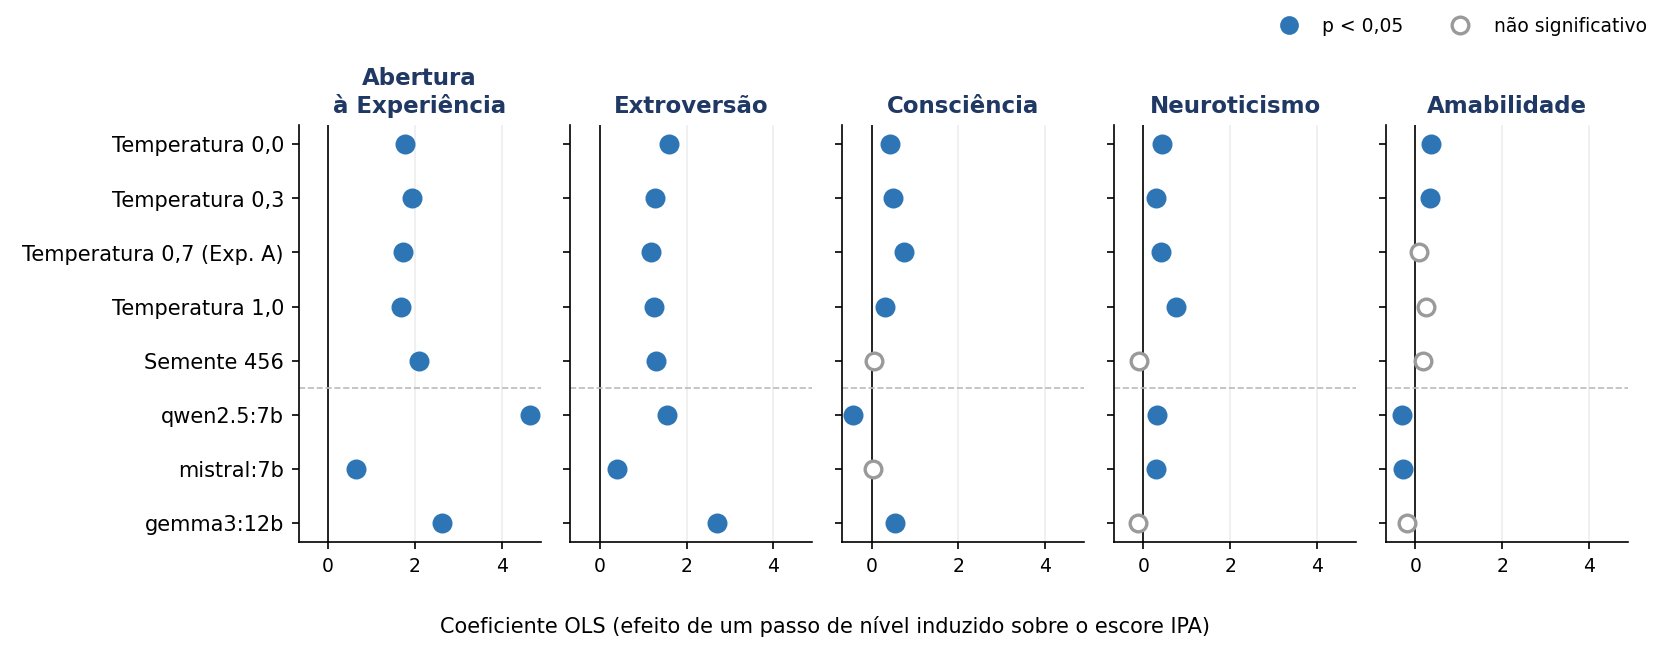
\includegraphics[width=\textwidth]{../resultados/figuras/fig11_robustez_coeficientes.png}
    \legend{Fonte: dados da pesquisa (Tabelas \ref{tab:robustez-temperatura}, \ref{tab:robustez-seed} e \ref{tab:robustez-modelos}). As cinco primeiras linhas usam o \texttt{llama3.1:8b}; a linha tracejada separa as rodadas com outros modelos. Círculos preenchidos: $p<0{,}05$.}
\end{figure}

Abertura à Experiência e Extroversão são positivas e significativas com
$p<0{,}001$ nas oito rodadas (Figura \ref{fig:robustez-coeficientes}). Consciência e Neuroticismo são significativos
na maior parte das rodadas, mas perdem a significância com o novo sorteio
e em parte dos modelos, e Consciência chega a inverter o sinal no
\texttt{qwen2.5:7b}. Amabilidade, sem efeito no Experimento A, aparece
com sinais opostos em diferentes rodadas. A interpretação desse padrão é
feita no Capítulo \ref{cap:discussao}.

% ============================================================================
% CAPÍTULO 5 — DISCUSSÃO
% ============================================================================
\chapter{Discussão}
\label{cap:discussao}

\section{Alinhamento com a literatura de referência}

\begin{table}[htb]
    \caption{Comparação dos achados com os artigos-base (Experimento A)}
    \label{tab:alinhamento-literatura}
    \centering
    \resizebox{\textwidth}{!}{%
    \begin{tabular}{lcccc}
        \toprule
        Traço & De Bortoli (2019) & Jiang et al. (2024) & Este estudo (Exp. A) & Análise de robustez \\
        \midrule
        Abertura à Experiência & Sig. positivo & Sig. positivo & Sig. positivo & Estável \\
        Extroversão            & Não sig.       & Otimismo (indireto) & Sig. positivo & Estável \\
        Consciência            & Não sig.       & Sig. negativo & Sig. positivo & Instável \\
        Neuroticismo           & Não sig.       & Sig. negativo & Sig. positivo & Instável \\
        Amabilidade             & Não sig.       & Papel mínimo & Não sig. & Sem efeito consistente \\
        \bottomrule
    \end{tabular}%
    }
    \legend{Fonte: elaborado pela autora a partir de \cite{debortoli2019}, \cite{jiangpengyan2024} e das Tabelas \ref{tab:ols} e \ref{tab:robustez-sintese} (Capítulo \ref{cap:resultados}).}
\end{table}

O efeito positivo e significativo de Abertura à Experiência sobre o
escore do IPA (Tabelas \ref{tab:spearman-ipa} e \ref{tab:ols}) é o
resultado mais robusto deste trabalho, por ser o único traço que replica
de forma consistente nos dois artigos-base. Em \citeonline{debortoli2019},
Abertura à Experiência foi o único traço estatisticamente significativo
para prever o perfil de risco real de estudantes em uma simulação de
investimento; em \citeonline{jiangpengyan2024}, o mesmo traço está entre
os dois com maior poder explicativo sobre o comportamento de investidores
reais, com efeito robusto sobre a alocação em ações nas três amostras do
estudo (Estados Unidos, Austrália e Alemanha). Os autores deste segundo
artigo decompõem o mecanismo por trás desse efeito: ao contrário do
Neuroticismo, cujo efeito passa pela leitura pessimista do cenário
econômico, o efeito de Abertura à Experiência não depende de crenças
sobre o mercado: decorre de uma disposição mais direta a aceitar risco,
independentemente de como o investidor avalia as perspectivas econômicas
(seção \ref{cap:referencial}).

Esse padrão, o mesmo traço na mesma direção em três contextos
metodologicamente distintos, é uma evidência relevante de robustez,
embora não uma prova. As três amostras diferem em praticamente tudo que
poderia gerar um resultado espúrio: sujeitos (estudantes brasileiros;
investidores reais americanos, majoritariamente homens brancos com mais
de 60 anos e patrimônio elevado; agentes de linguagem artificial),
variável dependente (perfil obtido por simulação de investimento real;
alocação declarada de carteira; escore de um questionário de perfil de
investidor respondido pelo próprio agente) e método estatístico
(regressão logística ordenada; OLS; correlação de Spearman e OLS). Um
efeito que se sustenta apesar dessa variação tem menor probabilidade de
ser um artefato de amostra, de instrumento ou de escolha estatística
específica de um dos três estudos. Ao mesmo tempo, essa convergência não
deve ser lida como evidência de que o agente de IA ``possui'' uma
disposição psicológica real ao risco equivalente à humana; ela mostra,
de forma mais modesta, que o pipeline de indução e mensuração deste
trabalho é capaz de reproduzir, ao menos para este traço, uma relação já
bem estabelecida na literatura, o que funciona também como uma validação
indireta do desenho experimental adotado, sem prejuízo das limitações de
validade externa desse tipo de simulação discutidas adiante neste
capítulo.

\textbf{Extroversão} não foi confirmada por \citeonline{debortoli2019}
(traço não significativo naquele estudo) e está apenas parcialmente
alinhada com \citeonline{jiangpengyan2024}, que encontram Extroversão
associada a expectativas mais otimistas sobre o mercado, mas sem efeito
significativo sobre a alocação real em ações; ou seja, o mecanismo que
Jiang et al. relatam para Extroversão é indireto e não se traduz em
comportamento, enquanto neste trabalho o efeito sobre o escore do IPA é
direto e significativo (coeficiente 1,19, p $<$ 0,001, Tabela
\ref{tab:ols}). Duas observações, feitas antes da análise de robustez,
relativizavam esse achado. Primeiro, na seleção do modelo, o efeito não
apareceu no \texttt{llama3.2:3b}, em que a manipulação de Extroversão foi
fraca ($\rho$=0,185; Tabela \ref{tab:comparacao-modelos}), o que era
compatível tanto com um achado real mascarado por manipulação ruim quanto
com um efeito restrito ao \texttt{llama3.1:8b}. Segundo, o
Experimento B (traço isolado, seção \ref{sec:exp-a-b}) não confirma este
achado com significância estatística ($\rho$=0,242, p=0,070, N=57, Tabela
\ref{tab:ipa-exp-b}), embora a magnitude seja parecida à do Experimento A (0,340),
o que sugere que a perda de significância pode refletir apenas o N bem
menor por traço no desenho isolado, não a ausência do efeito (discutido
em detalhe na seção \ref{sec:discussao-exp-b}). A análise de robustez e
generalização resolve essa dúvida a favor do efeito: com N=300 em cada
rodada, Extroversão foi positiva e significativa ($p<0,001$) nas quatro
temperaturas, com outro sorteio de perfis e nos três modelos abertos
adicionais (Tabela \ref{tab:robustez-sintese}), além de aparecer na mesma
direção nos dois modelos Nemotron. Isso responde às duas observações: o
efeito não é restrito ao \texttt{llama3.1:8b}, e sua ausência no
Experimento B é atribuível ao N menor. Por isso, Extroversão é tratada neste
trabalho como um efeito \textbf{robusto}, ao lado de Abertura à
Experiência, ainda que sem o respaldo dos dois artigos-base que Abertura
tem.

\textbf{Consciência e Neuroticismo}, diferentemente do que ocorria no
estudo piloto (BFI-10, onde nenhum dos dois era significativo), emergiram
como \textbf{significativos e positivos} na análise principal com BFI-44
(coeficientes 0,75 e 0,41 respectivamente, Tabela \ref{tab:ols}). Isso
muda a natureza da divergência em relação à literatura de referência: já
não é uma ausência de efeito (que seria consistente com
\citeonline{debortoli2019}, onde os dois também não são significativos),
e sim um efeito \textbf{na direção oposta} à relatada por
\citeonline{jiangpengyan2024}, que encontram Consciência e Neuroticismo
significativos e \textbf{negativos} sobre a alocação em ações, de forma
robusta nas três amostras do artigo (Estados Unidos, Austrália e
Alemanha; ver Capítulo \ref{cap:referencial}, seção "Síntese e hipóteses
de referência"). Ou seja, este trabalho diverge de \emph{ambos} os
artigos-base para esses dois traços: de De Bortoli et al. por encontrar
efeito onde eles não encontraram, e de Jiang et al. por encontrar o sinal
oposto ao deles. Não há, neste trabalho, dados que permitam decidir entre
duas explicações concorrentes para esse padrão: (i) o mecanismo humano
que Jiang et al. descrevem para Neuroticismo (leitura mais pessimista
do cenário econômico, que reduz alocação em ações) pode simplesmente
não se manifestar da mesma forma em um agente de LLM, cujas "crenças"
sobre o mercado não são geradas pelos mesmos processos cognitivos
descritos na literatura de finanças comportamentais; ou (ii) a descrição
de personalidade usada no \textit{prompt} para Consciência e Neuroticismo
(perfis\_personalidade.json) pode estar sendo interpretada pelo modelo de
um modo que favorece respostas mais decididas/arrojadas no IPA: por
exemplo, se o modelo associa "alta Consciência" (organização, disciplina,
orientação a objetivos) a uma postura mais assertiva de investimento, em
vez de à cautela esperada pela literatura humana. O Experimento B (seção
\ref{sec:discussao-exp-b}) mostra que, isolados, nenhum dos dois traços
mantém significância estatística, e Neuroticismo inverte de sinal
novamente ($\rho$=$-$0,116, Tabela \ref{tab:ipa-exp-b}). A análise de
robustez e generalização confirma essa fragilidade com amostras de mesmo
tamanho que a do Experimento A: com outro sorteio de perfis, os dois
coeficientes ficam próximos de zero e sem significância (0,048 e
$-$0,092, Tabela \ref{tab:robustez-seed}); entre temperaturas, oscilam
bastante de tamanho; e entre modelos, Consciência chega a inverter o
sinal (negativa no \texttt{qwen2.5:7b}) e cada um dos dois perde a
significância em pelo menos um modelo (Tabela \ref{tab:robustez-sintese}).
Por isso, Consciência e Neuroticismo são considerados neste trabalho
\textbf{resultados instáveis}: os efeitos aparecem no Experimento A, mas
dependem do sorteio, da temperatura e do modelo, e não devem ser
interpretados como uma relação geral entre esses traços e o perfil de
investidor simulado. Essa conclusão também relativiza a divergência com
\citeonline{jiangpengyan2024} discutida acima: sem um efeito estável, o
sinal oposto ao da literatura humana não pode ser tratado como um
achado substantivo sobre os agentes.

\textbf{Amabilidade} é o único traço sem nenhuma divergência a discutir:
não apresentou efeito significativo em nenhum dos três datasets deste
trabalho (piloto, Experimento A ou Experimento B, isolado ou não), o que
é consistente com os dois artigos-base: Amabilidade também não é
significativa em \citeonline{debortoli2019} e tem "papel mínimo" em
\citeonline{jiangpengyan2024}. Dos cinco traços investigados, é o único
em que os quatro estudos (os dois artigos-base e os dois desenhos deste
trabalho) concordam integralmente. Na análise de robustez, Amabilidade
aparece significativa em algumas rodadas, mas com sinais opostos
(positiva nas temperaturas 0,0 e 0,3, negativa no \texttt{qwen2.5:7b} e
no \texttt{mistral:7b}, Tabela \ref{tab:robustez-sintese}), o que reforça
a leitura de que não há um efeito consistente desse traço sobre o escore
do IPA.

\section{Indução simultânea vs. isolada: o Experimento B}
\label{sec:discussao-exp-b}

O Experimento B foi motivado por uma pergunta metodológica levantada
durante a orientação deste trabalho: será que induzir os 5 traços do Big
Five simultaneamente no mesmo \textit{prompt}, o desenho do Experimento
A, herdado da forma como a personalidade é medida em sujeitos humanos nos
dois artigos-base, que sempre possuem os 5 traços presentes em algum
nível, dilui ou confunde o sinal de cada traço individual, em
comparação a manipular apenas 1 traço por vez? O Experimento B testa essa
possibilidade diretamente, mantendo modelo e instrumento fixos e variando
apenas o desenho de indução (seção \ref{sec:exp-a-b}).

A resposta, com os dados deste trabalho, é dividida em duas partes. Na
\textbf{checagem de manipulação}, ou seja, na capacidade do modelo de
incorporar corretamente o nível de personalidade pedido, os dois
desenhos produzem resultados praticamente idênticos (Tabela
\ref{tab:manipulacao-exp-b}, Figura \ref{fig:exp-ab-manipulacao}): a correlação entre nível induzido e
autorrelato varia entre 0,81 e 0,93 tanto com os 5 traços variando juntos
quanto com apenas 1 variando isoladamente, sem diferença sistemática a
favor de nenhum dos dois desenhos. Isso é evidência direta \textbf{contra}
a hipótese de que a indução simultânea prejudica a capacidade do modelo
de incorporar cada traço: se houvesse esse tipo de interferência, seria
razoável esperar uma checagem de manipulação mais fraca no Experimento A
(5 traços competindo por "atenção" no mesmo \textit{prompt}) do que no B
(1 traço isolado), o que não se observa.

Já na \textbf{ligação com o escore do IPA} (Tabela \ref{tab:ipa-exp-b},
Figura \ref{fig:exp-ab-ipa}), o resultado é mais heterogêneo por traço. Abertura à Experiência não só
se mantém significativa isolada como fica mais forte ($\rho$=0,792 contra
0,530 no Experimento A); o achado mais robusto deste trabalho continua
robusto sob o desenho alternativo. Os outros quatro traços, no entanto,
perdem significância estatística quando isolados, incluindo os três que
emergiram como novidade no Experimento A (Extroversão, Consciência e
Neuroticismo, seção anterior). A explicação mais provável para essa
perda não é interferência entre traços, já descartada pela
checagem de manipulação idêntica nos dois desenhos, e sim
\textbf{poder estatístico}: o Experimento B tem, para cada traço
individual, entre 49 e 69 agentes (só os agentes em que aquele traço foi
sorteado como dominante), contra 300 no Experimento A. Para Extroversão,
por exemplo, a magnitude do efeito é semelhante nos dois desenhos (0,340
no A, 0,242 no B); a diferença é se esse coeficiente atinge o limiar de
significância com N=300 ou com N=57, não necessariamente se o efeito
existe. Neuroticismo é a exceção mais chamativa, invertendo de sinal
entre os dois desenhos (positivo no A, negativo no B, Tabela
\ref{tab:ipa-exp-b}); com N=69, essa inversão é compatível com
instabilidade de amostra pequena, mas também reforça que esse é o traço
com evidência menos consistente entre todos os testados neste trabalho.

Em síntese, o Experimento B responde à pergunta original de forma
específica: \textbf{induzir os 5 traços simultaneamente não parece
prejudicar a qualidade da indução em si}, mas o desenho isolado, do jeito
que foi implementado aqui (N pequeno por traço), \textbf{não tem poder
estatístico suficiente para confirmar ou refutar com segurança} os
achados secundários do Experimento A. Essa confirmação veio da análise
de robustez e generalização, discutida na próxima seção, que manteve
N=300 em cada rodada: Extroversão se confirmou, e Consciência e
Neuroticismo não.

\section{Robustez e generalização dos resultados}
\label{sec:discussao-robustez}

A análise de robustez e generalização (seção \ref{sec:resultados-robustez})
separa com clareza dois grupos de resultados. O primeiro é formado por
Abertura à Experiência e Extroversão, que elevam o escore do IPA em todas
as oito rodadas com N=300 (quatro temperaturas, dois sorteios de perfis e
quatro modelos abertos), sempre com $p<0,001$, e também nos dois modelos
Nemotron. Como essas rodadas variam, um de cada vez, o ruído da geração,
os perfis sorteados e o modelo, é pouco provável que esses dois efeitos
sejam produto de uma configuração específica do Experimento A. O segundo
grupo é formado pelos três traços de efeito menor (Consciência,
Neuroticismo e Amabilidade), cujos coeficientes mudam de significância e
de sinal entre rodadas. A temperatura, em particular, afeta mais o ruído
do que a direção dos efeitos: reduzi-la aumenta a fidelidade da
manipulação e o R², sem alterar quais traços têm efeito estável.

A generalização entre modelos, porém, vale para a \textit{direção} dos
dois efeitos estáveis, não para o \textit{nível} de risco declarado pelos
agentes. Com os mesmos perfis de personalidade, o perfil médio de
investidor vai de majoritariamente Moderado (\texttt{llama3.1:8b}) a
quase todo Arrojado (\texttt{mistral:7b}), e o mesmo agente recebe o
mesmo perfil do \texttt{llama3.1:8b} em apenas 20,3\% a 62,0\% dos casos,
conforme o modelo (Tabela \ref{tab:robustez-modelos-pareada}). O tamanho
dos efeitos também varia: o coeficiente de Abertura à Experiência vai de
0,632 (\texttt{mistral:7b}) a 4,643 (\texttt{qwen2.5:7b}). Na prática,
isso significa que uma simulação desse tipo pode indicar
\textit{quais} traços tornam um agente mais ou menos tolerante ao risco,
mas o perfil de investidor absoluto que ela atribui a uma personalidade
é, em grande parte, uma característica do modelo usado. Esse ponto é
relevante para qualquer uso de agentes de IA como substitutos de
respondentes humanos em avaliações de \textit{suitability}.

\section{Comparação com estudos de personalidade induzida em LLMs}
\label{sec:discussao-llm}

Entre os estudos revisados na seção \ref{sec:ref-llm-risco}, o de
\citeonline{borman2024} tem interseção direta com este trabalho. O
desenho de indução é essencialmente o mesmo do Experimento A: os cinco
traços do Big Five induzidos simultaneamente por instrução, cada um em
três níveis (Baixo, Médio e Alto), com a personalidade verificada por um
teste do próprio modelo dos cinco fatores antes da análise. A diferença
está no modo de compor a amostra (os autores usaram uma persona para cada
uma das 243 combinações possíveis; este trabalho sorteou os níveis de 300
agentes) e no modelo (ChatGPT 4.0, proprietário, contra, na análise
principal e nas rodadas com N=300, modelos abertos de 7 a 12 bilhões de
parâmetros). Os dois estudos também usam regressão
OLS para estimar a relação entre os traços e o comportamento. Essa
proximidade torna a comparação mais direta do que com os artigos-base,
que trabalham com sujeitos humanos.

A comparação mais informativa é com o questionário comportamental de
\citeonline{borman2024}, já que o IPA também é um questionário. Naquele
estudo, o questionário reproduziu a direção esperada pela literatura
humana para o apetite ao risco em Abertura à Experiência, Extroversão e
Neuroticismo, mas não em Consciência e Amabilidade. Neste trabalho,
Abertura e Extroversão aparecem na direção esperada e de forma estável,
convergindo com os autores; Consciência é instável e Amabilidade não
apresenta efeito consistente, o que também converge com a dificuldade
relatada por eles para esses dois traços no questionário. A divergência está em
Neuroticismo, que \citeonline{borman2024} reproduziram na direção
esperada e que, neste trabalho, é instável e, quando significativo,
positivo. Os autores relatam ainda que as personas representaram melhor
o comportamento humano em uma tarefa simulada de investimento do que no
questionário, inclusive acertando a direção dos cinco traços no apetite
ao risco. Esse resultado sugere que parte da instabilidade observada
neste trabalho nos traços de efeito menor pode estar ligada ao formato
de questionário, e motiva uma das recomendações de trabalho futuro
(Capítulo \ref{cap:conclusao}).

O estudo de \citeonline{hartley2025} converge com este trabalho em dois
pontos, apesar das diferenças de desenho (um traço induzido por vez,
modelos proprietários e risco medido por escolhas entre loterias). O
primeiro é o papel central de Abertura à Experiência: no GPT-4o, foi o
único traço com correlação significativa com os parâmetros de
sensibilidade ao risco, assim como é, neste trabalho, o traço de maior e
mais estável efeito sobre o IPA. O segundo é a dependência do modelo: os
autores observaram que a relação entre personalidade e risco não se
manteve nas variantes menores dos modelos e chegou a se inverter em
alguns deles, o que tem paralelo na variação entre modelos encontrada
aqui, tanto na seleção do modelo (seção \ref{sec:selecao-modelo}) quanto
na análise de generalização. Diferentemente de Hartley et al., porém,
este trabalho encontrou Extroversão com efeito estável em todos os
modelos testados, o que pode refletir a diferença de instrumento
(questionário de \textit{suitability} contra loterias) ou de forma de
indução (cinco traços simultâneos contra um traço por vez).

\section{O papel da checagem de manipulação}

Além da comparação entre desenhos de indução (seção anterior), a
comparação entre os 4 modelos de linguagem testados (Tabela
\ref{tab:comparacao-modelos}, seção \ref{sec:selecao-modelo}) é, em si,
um resultado deste trabalho: mostra que a qualidade da indução de
personalidade não é uniforme entre modelos, e que essa qualidade, não
apenas o tamanho do modelo isoladamente, é pré-requisito para
interpretar qualquer efeito sobre o IPA. O caso mais claro é Abertura à
Experiência: não significativa no \texttt{llama3.2:1b} ($\rho\approx$0,09
n.s.) nem no \texttt{llama3.2:3b} ($\rho$=0,077 n.s.) na checagem de
manipulação, e por consequência também não significativa na relação com
o IPA nesses dois modelos, mas fortemente incorporada no
\texttt{llama3.1:8b} ($\rho$=0,739 no piloto BFI-10; 0,913 no Experimento
A com BFI-44), onde o efeito sobre o IPA finalmente emerge com
significância. A interpretação mais direta é que os modelos menores não
"desconfirmam" a relação entre Abertura e perfil de investidor: eles
simplesmente falham em incorporar o traço de forma detectável, tornando
impossível testar a relação com esses dados. Sem a checagem de
manipulação, um resultado não significativo em um modelo pequeno poderia
ser lido (incorretamente) como evidência contra a hipótese de pesquisa,
quando na verdade reflete uma falha na etapa de indução, anterior à
pergunta de pesquisa em si.

\section{Vieses de resposta dos agentes}

Os quatro modelos testados na seleção do modelo apresentam vieses de resposta ao IPA que
independem da personalidade induzida. O mais consistente é o
\textbf{viés de centralidade}: os modelos da família Llama concentram
respostas no perfil Moderado, em proporção que diminui à medida que o
modelo cresce: aproximadamente 96\% no \texttt{llama3.2:1b}, 90\% no
\texttt{llama3.2:3b} e 78\% no \texttt{llama3.1:8b} (estudo piloto,
BFI-10). No Experimento A (BFI-44), o mesmo modelo (\texttt{llama3.1:8b})
concentrou 82,3\% dos agentes no perfil Moderado (Tabela
\ref{tab:distribuicao-ipa}), proporção semelhante à do piloto, o que
sugere que o viés de centralidade é uma característica do modelo, não do
instrumento de checagem de manipulação usado. O \texttt{gemma3:4b}
apresenta um viés distinto, de \textbf{conservadorismo}: no piloto
reduzido com esse modelo (N=30), 60\% dos agentes foram classificados
como Conservador e nenhum como Arrojado, mesmo com personalidades
induzidas variadas. A análise de generalização mostrou que cada modelo
tem um viés próprio, e não apenas os modelos menores: com os mesmos
perfis de personalidade, o \texttt{mistral:7b} concentrou 91,5\% dos
agentes no perfil Arrojado, o \texttt{gemma3:12b} teve a maior proporção
de Conservadores (24,0\%), e os dois modelos Nemotron responderam de
forma polarizada entre Conservador e Arrojado (Tabelas
\ref{tab:robustez-modelos} e \ref{tab:robustez-nemotron}).

Esses vieses são relevantes por dois motivos. Primeiro, como limitação de
validade: um modelo com viés de centralidade forte comprime a variância
do escore do IPA, o que reduz o poder estatístico disponível para
detectar qualquer efeito real da personalidade sobre esse escore,
prejudicando sistematicamente os modelos menores duas vezes (manipulação
mais fraca e menor variância na variável dependente). Segundo, como
achado metodológico por si só: a atenuação do viés de centralidade com o
aumento do modelo (96\%→90\%→78\%→82,3\%, aproximadamente) sugere que
não é só a capacidade de incorporar personalidade que melhora com modelos
maiores, mas também a disposição do modelo a dar respostas mais
extremas/decididas em geral, um comportamento de LLMs como sujeitos
simulados que merece atenção em trabalhos futuros que usem esse tipo de
questionário de múltipla escolha com agentes de IA.

\section{Limitações do estudo}

\begin{itemize}
    \item \textbf{O instrumento de autorrelato da análise principal não
    corresponde exatamente ao de nenhum dos dois artigos-base}. O BFI-10,
    usado no estudo piloto e na comparação entre modelos, é o mesmo
    instrumento (e a mesma tradução) usados por
    \citeonline{debortoli2019}; o BFI-44, usado na análise principal
    (Experimentos A e B), em uma versão em português que não é idêntica
    à adaptação validada para o Brasil por \citeonline{andrade2008}, não
    corresponde exatamente nem ao BFI-10
    de De Bortoli et al. nem ao SAPA-20 de \citeonline{jiangpengyan2024}.
    Essa é uma limitação real de comparabilidade introduzida pela
    migração de instrumento (seção \ref{sec:exp-a-b}), mitigada, mas
    não eliminada, pelo fato de os itens do BFI-44 medirem os mesmos 5
    traços do mesmo modelo teórico (Big Five), com escala de resposta
    idêntica à do BFI-10;
    \item \textbf{Vieses de resposta do modelo}, sobretudo a
    concentração de respostas no perfil Moderado, discutidos na seção
    anterior, comprimem a variância da variável dependente e reduzem o
    poder estatístico disponível para detectar efeitos reais da
    personalidade;
    \item \textbf{Os cortes de classificação do perfil IPA
    (Conservador/\allowbreak Moderado/\allowbreak Arrojado) são uma operacionalização própria
    deste trabalho}, não publicada no artigo original de referência para
    o questionário (seção \ref{sec:ipa-pontuacao}); outra
    escolha de corte poderia produzir uma distribuição de perfis
    diferente, embora não afete as correlações de Spearman nem os
    coeficientes da OLS, calculados sobre o escore contínuo;
    \item \textbf{Validade externa}: os sujeitos deste trabalho são
    agentes de linguagem artificial, não investidores reais: os
    achados dizem respeito a como um modelo de linguagem específico
    responde quando instruído a simular uma personalidade, não
    necessariamente a como pessoas reais com essas personalidades se
    comportariam;
    \item \textbf{Abrangência dos modelos testados}: a análise de
    generalização cobriu quatro modelos abertos de 7 a 12 bilhões de
    parâmetros com N=300 e dois modelos maiores apenas em piloto (N=30),
    acessados por uma cota gratuita de API. Modelos proprietários de
    grande porte (como os das famílias GPT, Claude e Gemini) não foram
    testados, e um modelo previsto para o piloto (Gemma 4 31B) não pôde
    ser incluído por indisponibilidade do provedor gratuito; os
    resultados podem não se estender a esses modelos;
    \item \textbf{Questionário em vez de tarefa comportamental}: o perfil
    de investidor foi medido por um questionário de autorrelato (IPA), e
    não pelo comportamento do agente em uma tarefa de investimento. Em
    \citeonline{borman2024}, personas de LLM representaram melhor o
    comportamento humano em uma tarefa simulada do que em um
    questionário, o que sugere que o formato do instrumento pode ter
    contribuído para a instabilidade dos efeitos menores;
    \item \textbf{N pequeno por traço no Experimento B} (49 a 69 agentes,
    contra 300 no Experimento A), como discutido na seção
    \ref{sec:discussao-exp-b}, isso limita a capacidade desse experimento
    de confirmar ou refutar com segurança os efeitos secundários do
    Experimento A, papel que coube à análise de robustez e
    generalização.
\end{itemize}

% ============================================================================
% CAPÍTULO 6 — CONCLUSÃO
% ============================================================================
\chapter{Conclusão}
\label{cap:conclusao}

A pergunta de pesquisa que orientou este trabalho (Capítulo
\ref{cap:introducao}) era se níveis induzidos de personalidade Big Five em
agentes de inteligência artificial predizem o escore do questionário de
perfil de investidor (IPA). A resposta, com os dados da análise principal
(Experimento A, BFI-44, N=300, \texttt{llama3.1:8b}), é afirmativa, porém
parcial: o modelo com os cinco níveis induzidos explica 45,9\% da
variância do escore IPA ($R^2=0{,}459$; $p<0{,}001$; Tabela \ref{tab:ols}),
mas apenas dois dos cinco traços, Abertura à Experiência e Extroversão,
têm efeito que se sustenta em todas as rodadas da análise de robustez e
generalização. As três questões de pesquisa definidas na introdução
detalham essa resposta.

\section{Respostas às questões de pesquisa}

\textbf{RQ1: Os LLMs conseguem simular consistentemente os traços de
personalidade solicitados?} Sim, mas não em qualquer modelo. No
Experimento A, a correlação entre o nível induzido e o autorrelato no
BFI-44 ficou entre 0,813 e 0,929 nos cinco traços (Tabela
\ref{tab:manipulacao}), com valores semelhantes quando cada traço foi
induzido isoladamente (Experimento B, Tabela \ref{tab:manipulacao-exp-b}),
em todas as temperaturas testadas e nos demais modelos da análise de
generalização, de 7 a 12 bilhões de parâmetros (seção
\ref{sec:resultados-robustez}). A indução também
se mostrou específica: cada nível induzido se reflete sobretudo no
próprio traço, e a correlação entre os traços autorrelatados foi baixa
(média de 0,110 em módulo; seção \ref{sec:resultados-intercorrelacao}).
Essa consistência, porém, não é garantida em qualquer modelo: o modelo
mais leve testado na seleção do modelo (\texttt{llama3.2:1b}) não
incorporou nenhum dos cinco traços de forma detectável, e o
\texttt{llama3.2:3b} incorporou apenas parte deles (seção
\ref{sec:selecao-modelo}). Dentro da família Llama, a fidelidade cresceu
com o tamanho do modelo, mas o \texttt{gemma3:4b}, com 4,3 bilhões de
parâmetros, também incorporou os cinco traços no teste reduzido (N=30),
o que indica que a capacidade de simular a personalidade depende do
modelo, e não apenas do seu porte.

\textbf{RQ2: Quais associações entre personalidade induzida e perfil de
investidor são robustas?} As de \textbf{Abertura à Experiência} e
\textbf{Extroversão}, ambas positivas: níveis induzidos mais altos desses
traços associam-se a escores IPA mais altos (mais arrojados). As duas
foram significativas, com $p<0{,}001$, nas oito rodadas com 300 agentes
da análise de robustez e generalização (o Experimento A e mais sete
rodadas: três temperaturas adicionais, um novo sorteio de perfis e três
outros modelos abertos; Tabela \ref{tab:robustez-sintese}) e aparecem na
mesma direção nos dois modelos Nemotron. Abertura à Experiência é, além
disso, o único traço com efeito significativo que converge com os dois
artigos-base
\cite{debortoli2019,jiangpengyan2024} e com o estudo de
\citeonline{hartley2025}, e o único que se manteve significativo quando
induzido isoladamente (Experimento B). Os efeitos de
\textbf{Consciência} e \textbf{Neuroticismo}, significativos no
Experimento A, são instáveis: perdem significância com outro
sorteio de perfis e mudam de significância ou de sinal entre modelos;
com a temperatura, variam em intensidade. \textbf{Amabilidade} não tem
efeito consistente.

\textbf{RQ3: Em que medida essas associações e os perfis financeiros
dependem do modelo e dos parâmetros de geração?} A \textit{direção} das
associações robustas depende pouco: Abertura à Experiência e Extroversão
mantêm o sinal e a significância em todas as temperaturas e em todos os
modelos da análise de generalização. A temperatura afeta principalmente o
ruído: reduzi-la de 0,7 para 0,0 eleva o $R^2$ de 0,459 para 0,707 e torna
a manipulação mais fiel, sem mudar o sinal e a significância de Abertura
à Experiência e de Extroversão; Amabilidade, porém, torna-se
significativa nas temperaturas mais baixas, o que mostra que uma única
configuração de geração pode indicar efeitos que não se sustentam. Já o
\textit{tamanho} dos efeitos e, sobretudo, o \textit{perfil de investidor
absoluto} dependem fortemente do modelo: com os mesmos perfis de
personalidade, a proporção de agentes Arrojados vai de 14,0\%
(\texttt{llama3.1:8b}) a 91,5\% (\texttt{mistral:7b}), e o perfil
atribuído a um mesmo agente coincide com o obtido no \texttt{llama3.1:8b}
em 20,3\% a 62,0\% dos casos, conforme o modelo. Os efeitos instáveis
(Consciência e Neuroticismo), assim como o de Amabilidade, são justamente
os que mais dependem do modelo e da geração.

Esse padrão de resultado (dois efeitos estáveis cercados de efeitos
menores que não se sustentam) delimita o que este tipo de simulação pode
oferecer. A convergência de Abertura à Experiência entre um estudo com
124 estudantes, um estudo com 3.325 investidores reais e a simulação com
agentes de IA deste trabalho é a evidência mais forte que este trabalho
produz em favor de uma resposta afirmativa à pergunta de pesquisa. Essa
convergência, contudo, não demonstra que um agente de linguagem
``possua'' personalidade no sentido psicológico do termo; o que ela
mostra é que, com indução e checagem de manipulação, a simulação
reproduziu a direção de uma relação relatada nos dois estudos com
humanos.

\section{Objetivos específicos}

Retomando os objetivos específicos definidos na introdução, um a um:

\begin{enumerate}
    \item \textbf{Induzir e verificar níveis de personalidade por
    instrução}: atingido. A checagem de manipulação confirmou incorporação
    forte e estatisticamente significativa dos cinco traços tanto no
    Experimento A ($\rho$ entre 0,813 e 0,929, Tabela \ref{tab:manipulacao})
    quanto no Experimento B ($\rho$ entre 0,837 e 0,930 por traço, Tabela
    \ref{tab:manipulacao-exp-b}), com o \texttt{llama3.1:8b} escolhido por
    ter sido, na seleção do modelo (feita com o BFI-10), o único que
    reuniu manipulação significativa nos cinco traços (forte em quatro
    deles e moderada em Extroversão), N suficiente para inferência e
    variância adequada no escore do IPA;
    \item \textbf{Aplicar o IPA e obter escore contínuo e classificação
    categórica}: atingido. Os 300 agentes do Experimento A foram
    classificados, pelo escore total do IPA (8 perguntas, 8 a 32 pontos,
    seção \ref{sec:ipa-pontuacao}), em 3,7\% Conservador, 82,3\%
    Moderado e 14,0\% Arrojado (Tabela \ref{tab:distribuicao-ipa}); para a
    análise estatística, foi usado o escore contínuo restrito às
    perguntas 2 a 8 (média 17,58, desvio padrão 2,72), que exclui a
    pergunta 1, cuja resposta foi sorteada;
    \item \textbf{Testar a associação estatística entre nível induzido e
    escore do IPA}: atingido para os cinco traços, por correlação de
    Spearman (Tabela \ref{tab:spearman-ipa}) e regressão OLS (Tabela
    \ref{tab:ols}), com quatro dos cinco coeficientes estatisticamente
    significativos no Experimento A, dois deles estáveis (RQ2);
    \item \textbf{Comparar os achados com \citeonline{debortoli2019} e
    \citeonline{jiangpengyan2024}}: atingido (seção
    \ref{sec:discussao-alinhamento}). Abertura à Experiência converge com
    os dois artigos-base; Amabilidade converge com
    \citeonline{debortoli2019} e com a ausência de efeito sobre a alocação
    em \citeonline{jiangpengyan2024}; Extroversão diverge de
    \citeonline{debortoli2019}, mas é compatível com a menor aversão ao
    risco declarada relatada por \citeonline{jiangpengyan2024}; e
    Consciência e Neuroticismo, além de divergirem dos dois artigos-base,
    mostraram-se instáveis, o que impede tratar essa divergência como um
    achado substantivo;
    \item \textbf{Comparar diferentes modelos de linguagem quanto à
    qualidade da indução}: atingido (Capítulo \ref{cap:metodologia}, seção
    \ref{sec:selecao-modelo}, e Capítulo \ref{cap:resultados}, seção
    \ref{sec:resultados-robustez}). Na seleção do modelo, a qualidade da
    indução cresceu com o tamanho do modelo dentro da família Llama; na
    análise de generalização, todos os modelos de 7 bilhões de parâmetros
    ou mais incorporaram os cinco traços;
    \item \textbf{Testar se a indução simultânea dos cinco traços afeta a
    qualidade da indução ou a força da associação com o IPA}: atingido
    (Experimento B, seção \ref{sec:discussao-exp-b}). A indução simultânea
    não prejudica a checagem de manipulação em si, mas o desenho isolado,
    com N entre 49 e 69 por traço, não teve poder estatístico suficiente
    para confirmar ou refutar com segurança os efeitos secundários do
    Experimento A;
    \item \textbf{Avaliar a robustez e a generalização das associações}:
    atingido (seções \ref{sec:resultados-robustez} e
    \ref{sec:discussao-robustez}). Abertura à Experiência e Extroversão se
    mantiveram significativas em todas as temperaturas, sorteios e modelos
    da análise de robustez e generalização; Consciência e Neuroticismo,
    não.
\end{enumerate}

\section{Contribuições}

Este trabalho contribui em três frentes. Em primeiro lugar, produz
evidência de que agentes de IA baseados em LLM, quando adequadamente
induzidos e submetidos a uma checagem de manipulação, reproduzem
parcialmente a direção de relações já documentadas entre personalidade
Big Five e comportamento de risco financeiro: a convergência de Abertura
à Experiência entre os dois artigos-base e este trabalho é o achado
central nesse sentido, ao passo que a instabilidade dos demais traços
delimita com igual clareza até onde essa replicação se sustenta.

Em segundo lugar, o trabalho aplica e documenta uma metodologia replicável
para o uso de LLMs como sujeitos simulados em pesquisa comportamental:
indução de personalidade por instrução, checagem de manipulação
obrigatória antes de interpretar qualquer efeito sobre a variável
dependente e uma análise de robustez e generalização que repete o
experimento variando, um de cada vez, a temperatura, o sorteio de perfis
e o modelo. Essa análise mostrou que um efeito estatisticamente
significativo em uma única configuração (como Consciência e Neuroticismo
no Experimento A) pode não se sustentar em outras, e que, sem ela, este
trabalho teria apresentado quatro efeitos onde apenas dois são estáveis.
A comparação entre modelos na seleção do modelo também mostrou que
modelos menores (\texttt{llama3.2:1b} e \texttt{llama3.2:3b}) não
atingiram manipulação confiável dos cinco traços (Tabela
\ref{tab:comparacao-modelos}), o que recomenda verificar a manipulação
antes de usar um modelo nesse tipo de simulação.

Em terceiro lugar, a comparação entre modelos mostra que o modelo de
linguagem não é um detalhe de implementação: ele determina se a indução
funciona (o modelo mais leve testado não incorporou nenhum traço) e,
mesmo entre modelos em que a indução funciona, determina o perfil de
investidor absoluto atribuído a uma mesma personalidade. O perfil
absoluto obtido nesse tipo de simulação deve, portanto, ser reportado
como propriedade do modelo usado, e não como estimativa do comportamento
de investidores.

\section{Recomendações para trabalhos futuros}

\begin{itemize}
    \item Substituir o questionário de perfil de investidor por uma
    \textbf{tarefa comportamental de investimento}, ou complementá-lo com
    ela, em que o agente toma decisões (por exemplo, alocar um valor entre
    ativos com risco e retorno conhecidos) em vez de declarar
    preferências. Em \citeonline{borman2024}, personas de LLM
    representaram melhor o comportamento humano nesse formato do que em
    questionário, e essa mudança pode reduzir a instabilidade observada
    nos traços de efeito menor;
    \item Estender a análise de generalização a modelos maiores, inclusive
    proprietários, com N suficiente para inferência, já que os modelos
    Nemotron foram testados apenas em caráter exploratório (N=30);
    \item Adaptar o IPA, ou adotar outro instrumento de tolerância ao
    risco validado, ao contexto específico de agentes de IA, removendo ou
    ajustando itens originalmente pensados para respondentes humanos (como
    a pergunta de faixa etária, cuja resposta foi atribuída aleatoriamente
    neste trabalho por não fazer sentido que o modelo a respondesse; seção
    \ref{sec:limitacoes-pipeline}).
\end{itemize}

\pagebreak

%%%%%%%%%%%%%%%%%%%%%%%%%%%%%%%%%%%%%%%%%%%%%%%%%%%%%%%%%%%%
% B I B L I O G R A F I A
%%%%%%%%%%%%%%%%%%%%%%%%%%%%%%%%%%%%%%%%%%%%%%%%%%%%%%%%%%%%
\makebibspage{referencias}

% Sem apêndices nem anexos: a pedido do orientador, os instrumentos (BFI-10,
% BFI-44, IPA), a regra de pontuação do IPA e os prompts ficam no Cap. 3, e a
% verificação do sorteio no Cap. 4. Os antigos postextual/apendices.tex e
% postextual/anexos.tex podem ser recuperados pelo histórico do git.

\end{document}
